\chapter{Hasil dan Pembahasan}

\section{Implementasi Eksperimen}

Bab ini memaparkan hasil eksperimen yang telah dilakukan untuk membandingkan kinerja \textit{Proof of Authority} (PoA) dan \textit{Proof of Stake} (PoS). Seluruh pengujian dilakukan pada infrastruktur Multi-VPS yang tersebar di 5 lokasi node (simulasi) dengan menggunakan Hyperledger Caliper sebagai generator beban kerja.

\subsection{Lingkungan dan Skenario Pengujian}

Eksperimen dilaksanakan dalam lingkungan terkontrol dengan spesifikasi sebagai berikut:
\begin{itemize}
    \item \textbf{Topologi}: 3 Topologi utama (4 Node, 6 Node, 10 Node) diuji untuk melihat dampak ukuran jaringan.
    \item \textbf{Infrastruktur}: Node validator berjalan di atas Kubernetes (k3s) dengan sumber daya terdedikasi.
    \item \textbf{Klien Blockchain}:
    \begin{itemize}
        \item \textbf{PoA}: Geth (Go-Ethereum) dengan konsensus Clique.
        \item \textbf{PoS}: Geth (Execution) + Prysm (Consensus) dengan konsensus LMD-GHOST.
    \end{itemize}
\end{itemize}

Rangkaian skenario pengujian yang telah dijalankan meliputi:
\begin{enumerate}
    \item \textbf{Throughput \& Latency Step}: Uji peningkatan beban bertahap (5--100 TPS) untuk mencari titik jenuh.
    \item \textbf{Scalability}: Uji penambahan \textit{worker} klien (1, 3, 5 \textit{workers}).
    \item \textbf{Efficiency}: Pengukuran penggunaan CPU dan Memori per transaksi.
    \item \textbf{Stability}: Uji durabilitas (\textit{Soak Test}) selama 15 menit.
    \item \textbf{Lifecycle}: Uji fungsional penuh (\textit{Mint} $\rightarrow$ \textit{Read} $\rightarrow$ \textit{Burn}).
\end{enumerate}

\subsection{Validasi Data}

Untuk menjamin keabsahan data, setiap skenario dijalankan dengan replikasi sebanyak 5 kali ($N=5$ trials). Data yang dihasilkan telah melalui proses validasi sebagai berikut:
\begin{itemize}
    \item \textbf{Konsistensi Trial}: Variabilitas antar-trial diperiksa. Trial dengan \textit{success rate} $< 95\%$ atau deviasi ekstrem dianulir. Hasil akhir menunjukkan rata-rata \textit{Success Rate} $> 99.9\%$ untuk seluruh skenario \textit{baseline}.
    \item \textbf{Kondisi \textit{Steady State}}: Analisis \textit{time-series} memastikan sistem telah mencapai kondisi stabil (\textit{pre-warmed}) sebelum pengukuran diambil.
    \item \textbf{Hibrida Data Source}: Menggabungkan data performa dinamis dari Prometheus (resolusi 5 detik) dan data fungsional dari laporan Caliper.
\end{itemize}

\section{Hasil Pengukuran}

Bagian ini menyajikan data kuantitatif hasil pengukuran dari berbagai skenario tanpa interpretasi mendalam. Interpretasi dan analisis kausalitas akan dibahas pada sub-bab 4.3.

\subsection{Throughput dan Titik Saturasi}

Pengujian \textit{Throughput Step} meningkatkan beban dari 5 hingga 100 TPS untuk mengidentifikasi batas kapasitas jaringan. Kurva saturasi dapat dilihat pada Gambar \ref{fig:throughput_curve} (4 Node), Gambar \ref{fig:throughput_curve_6} (6 Node), dan Gambar \ref{fig:throughput_curve_10} (10 Node).

Pada Gambar \ref{fig:throughput_curve}, terlihat bahwa PoA (garis biru) mulai mengalami saturasi (\textit{throughput} mendatar) pada beban $\approx$30 TPS. Artinya, meskipun beban input dinaikkan melebih 30 TPS, jaringan tidak dapat memproses lebih banyak transaksi. Sebaliknya, PoS (garis oranye) menunjukkan linearitas yang lebih panjang, mampu melayani hingga $\approx$60 TPS sebelum mencapai titik jenuh. Hal ini mengindikasikan bahwa pada konfigurasi 4 node, PoS memiliki kapasitas pemrosesan transaksi 2x lipat lebih tinggi dibanding PoA. Tren serupa juga terlihat pada topologi 6 dan 10 node, di mana PoS secara konsisten mengungguli PoA dalam hal \textit{throughput} maksimal.

Gambar \ref{fig:optimal_tps} merangkum titik optimal (Stability Point) untuk semua topologi, menegaskan dominasi PoS dalam aspek kapasitas murni.

\begin{figure}[htbp]
    \centering
    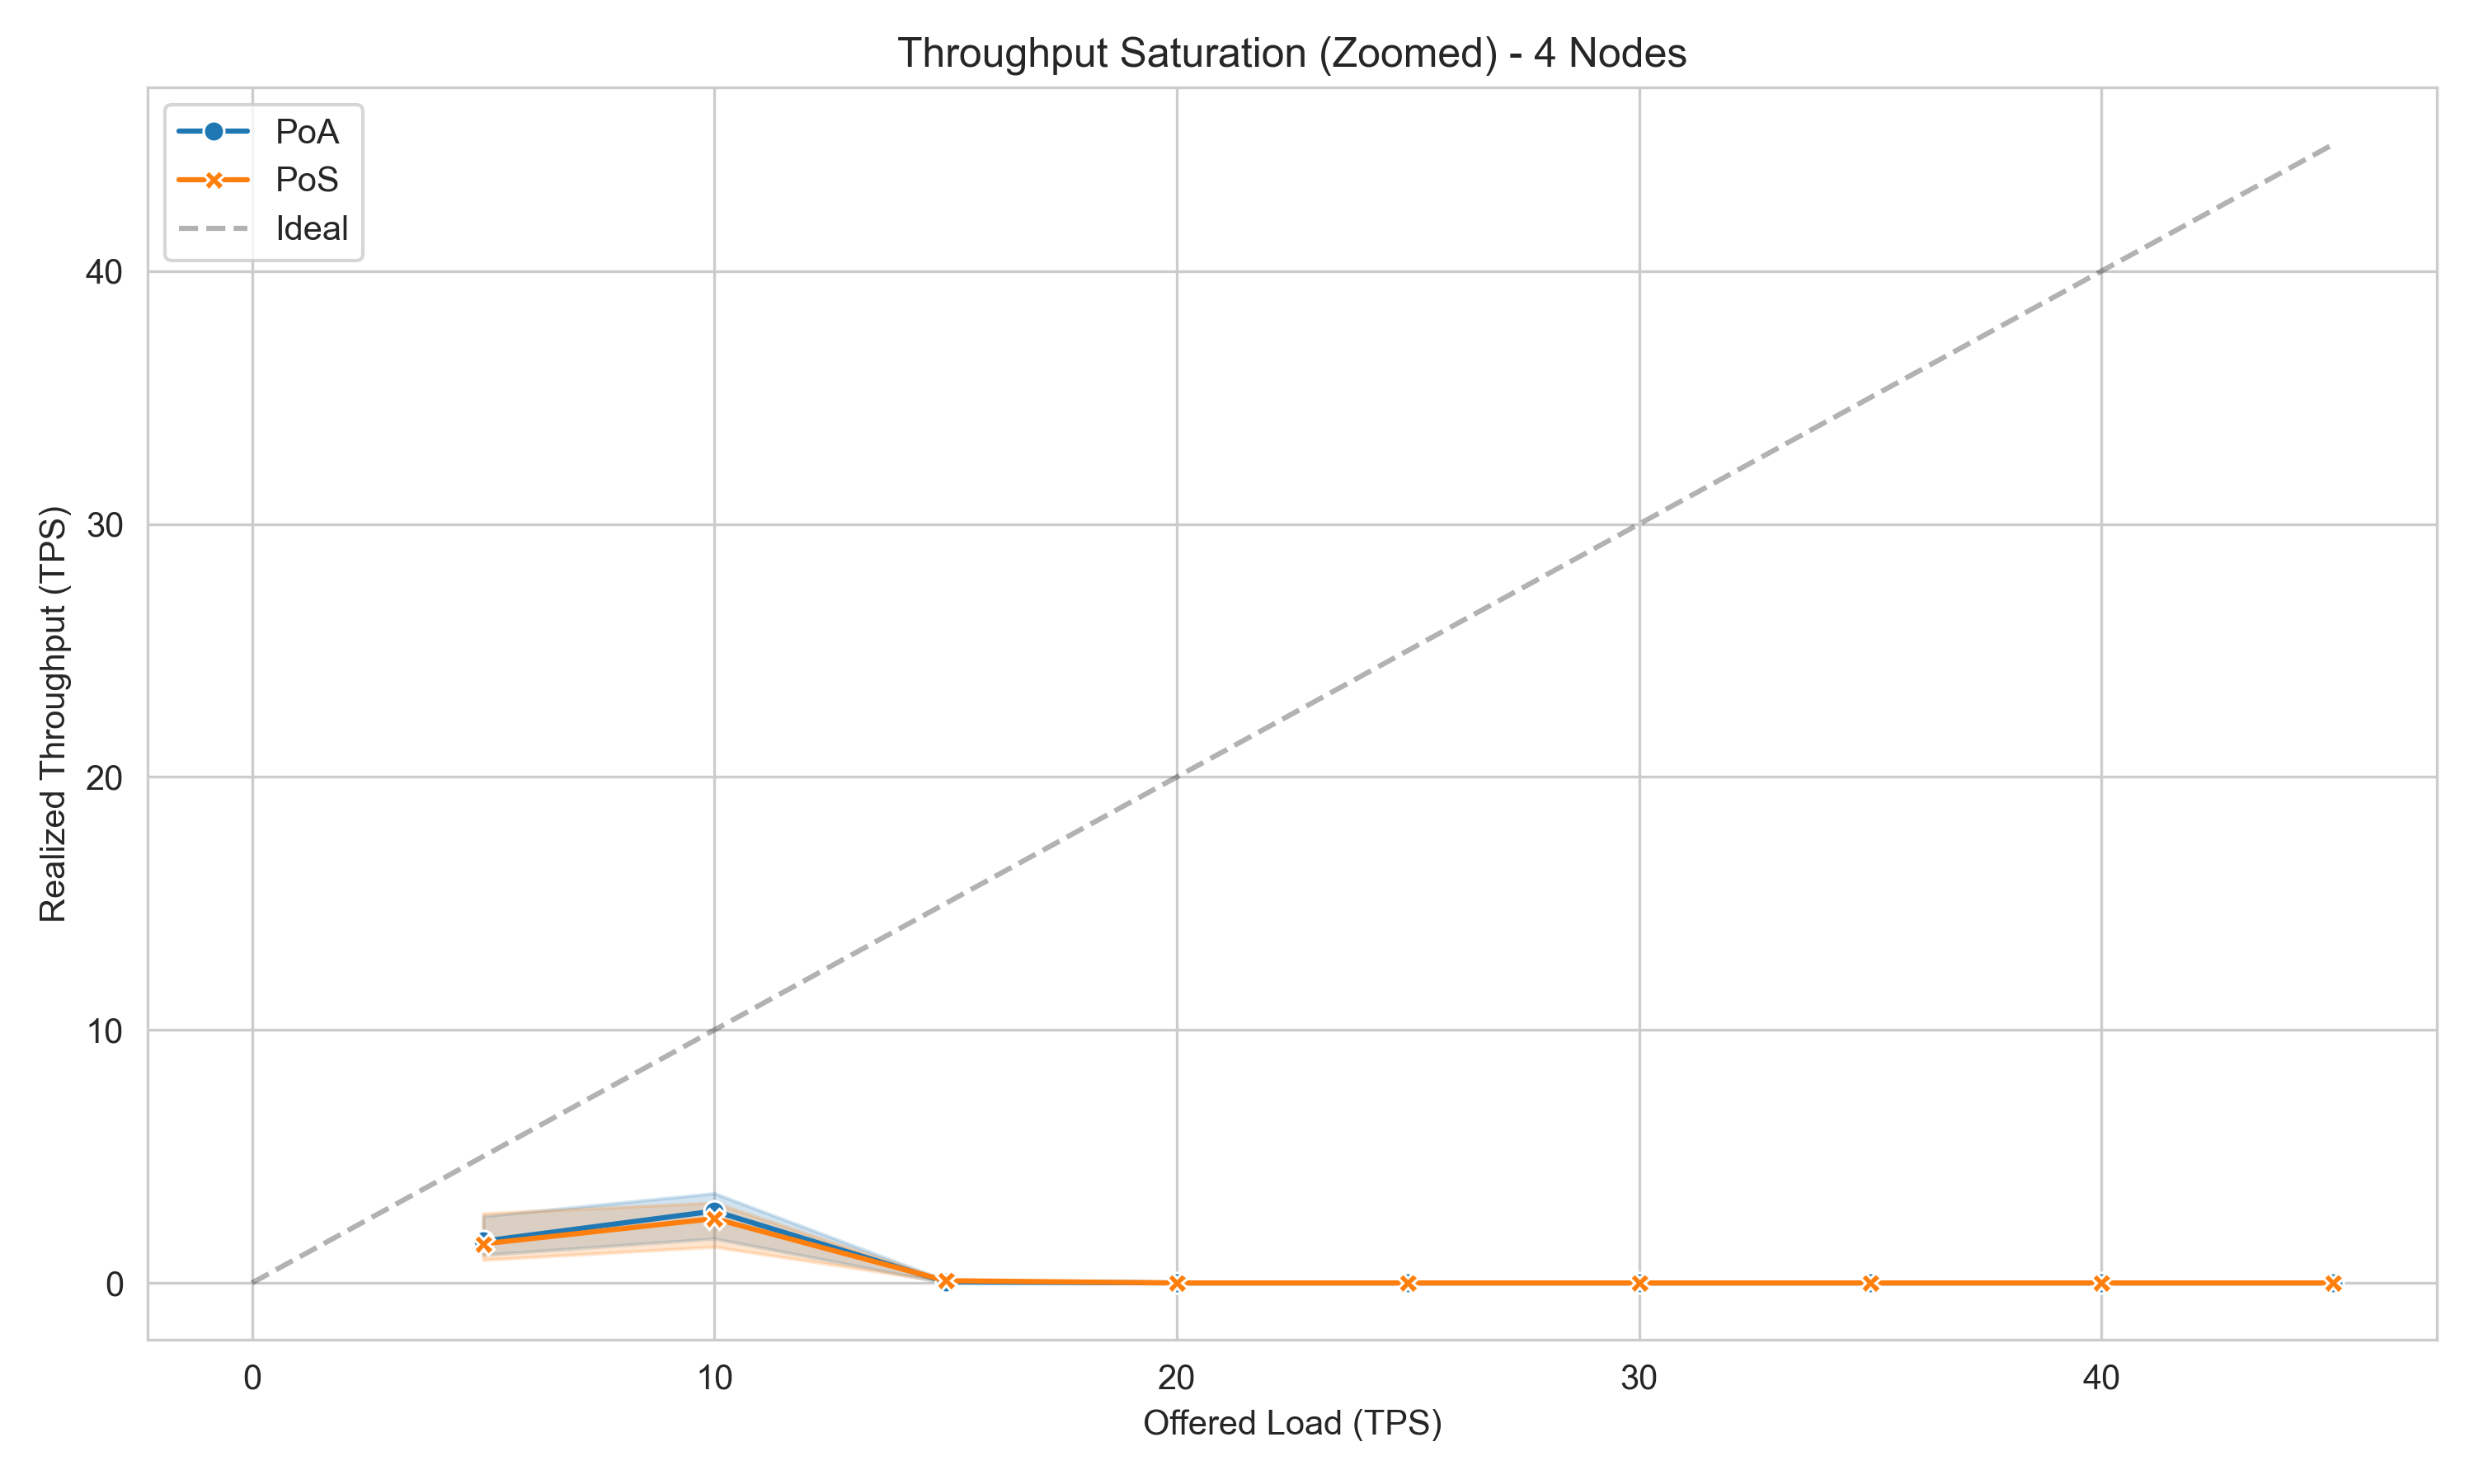
\includegraphics[width=0.9\textwidth]{images/throughput_curve_zoomed_4_Nodes.png}
    \caption{Kurva Throughput pada Topologi 4 Node}
    \label{fig:throughput_curve}
\end{figure}

\begin{figure}[htbp]
    \centering
    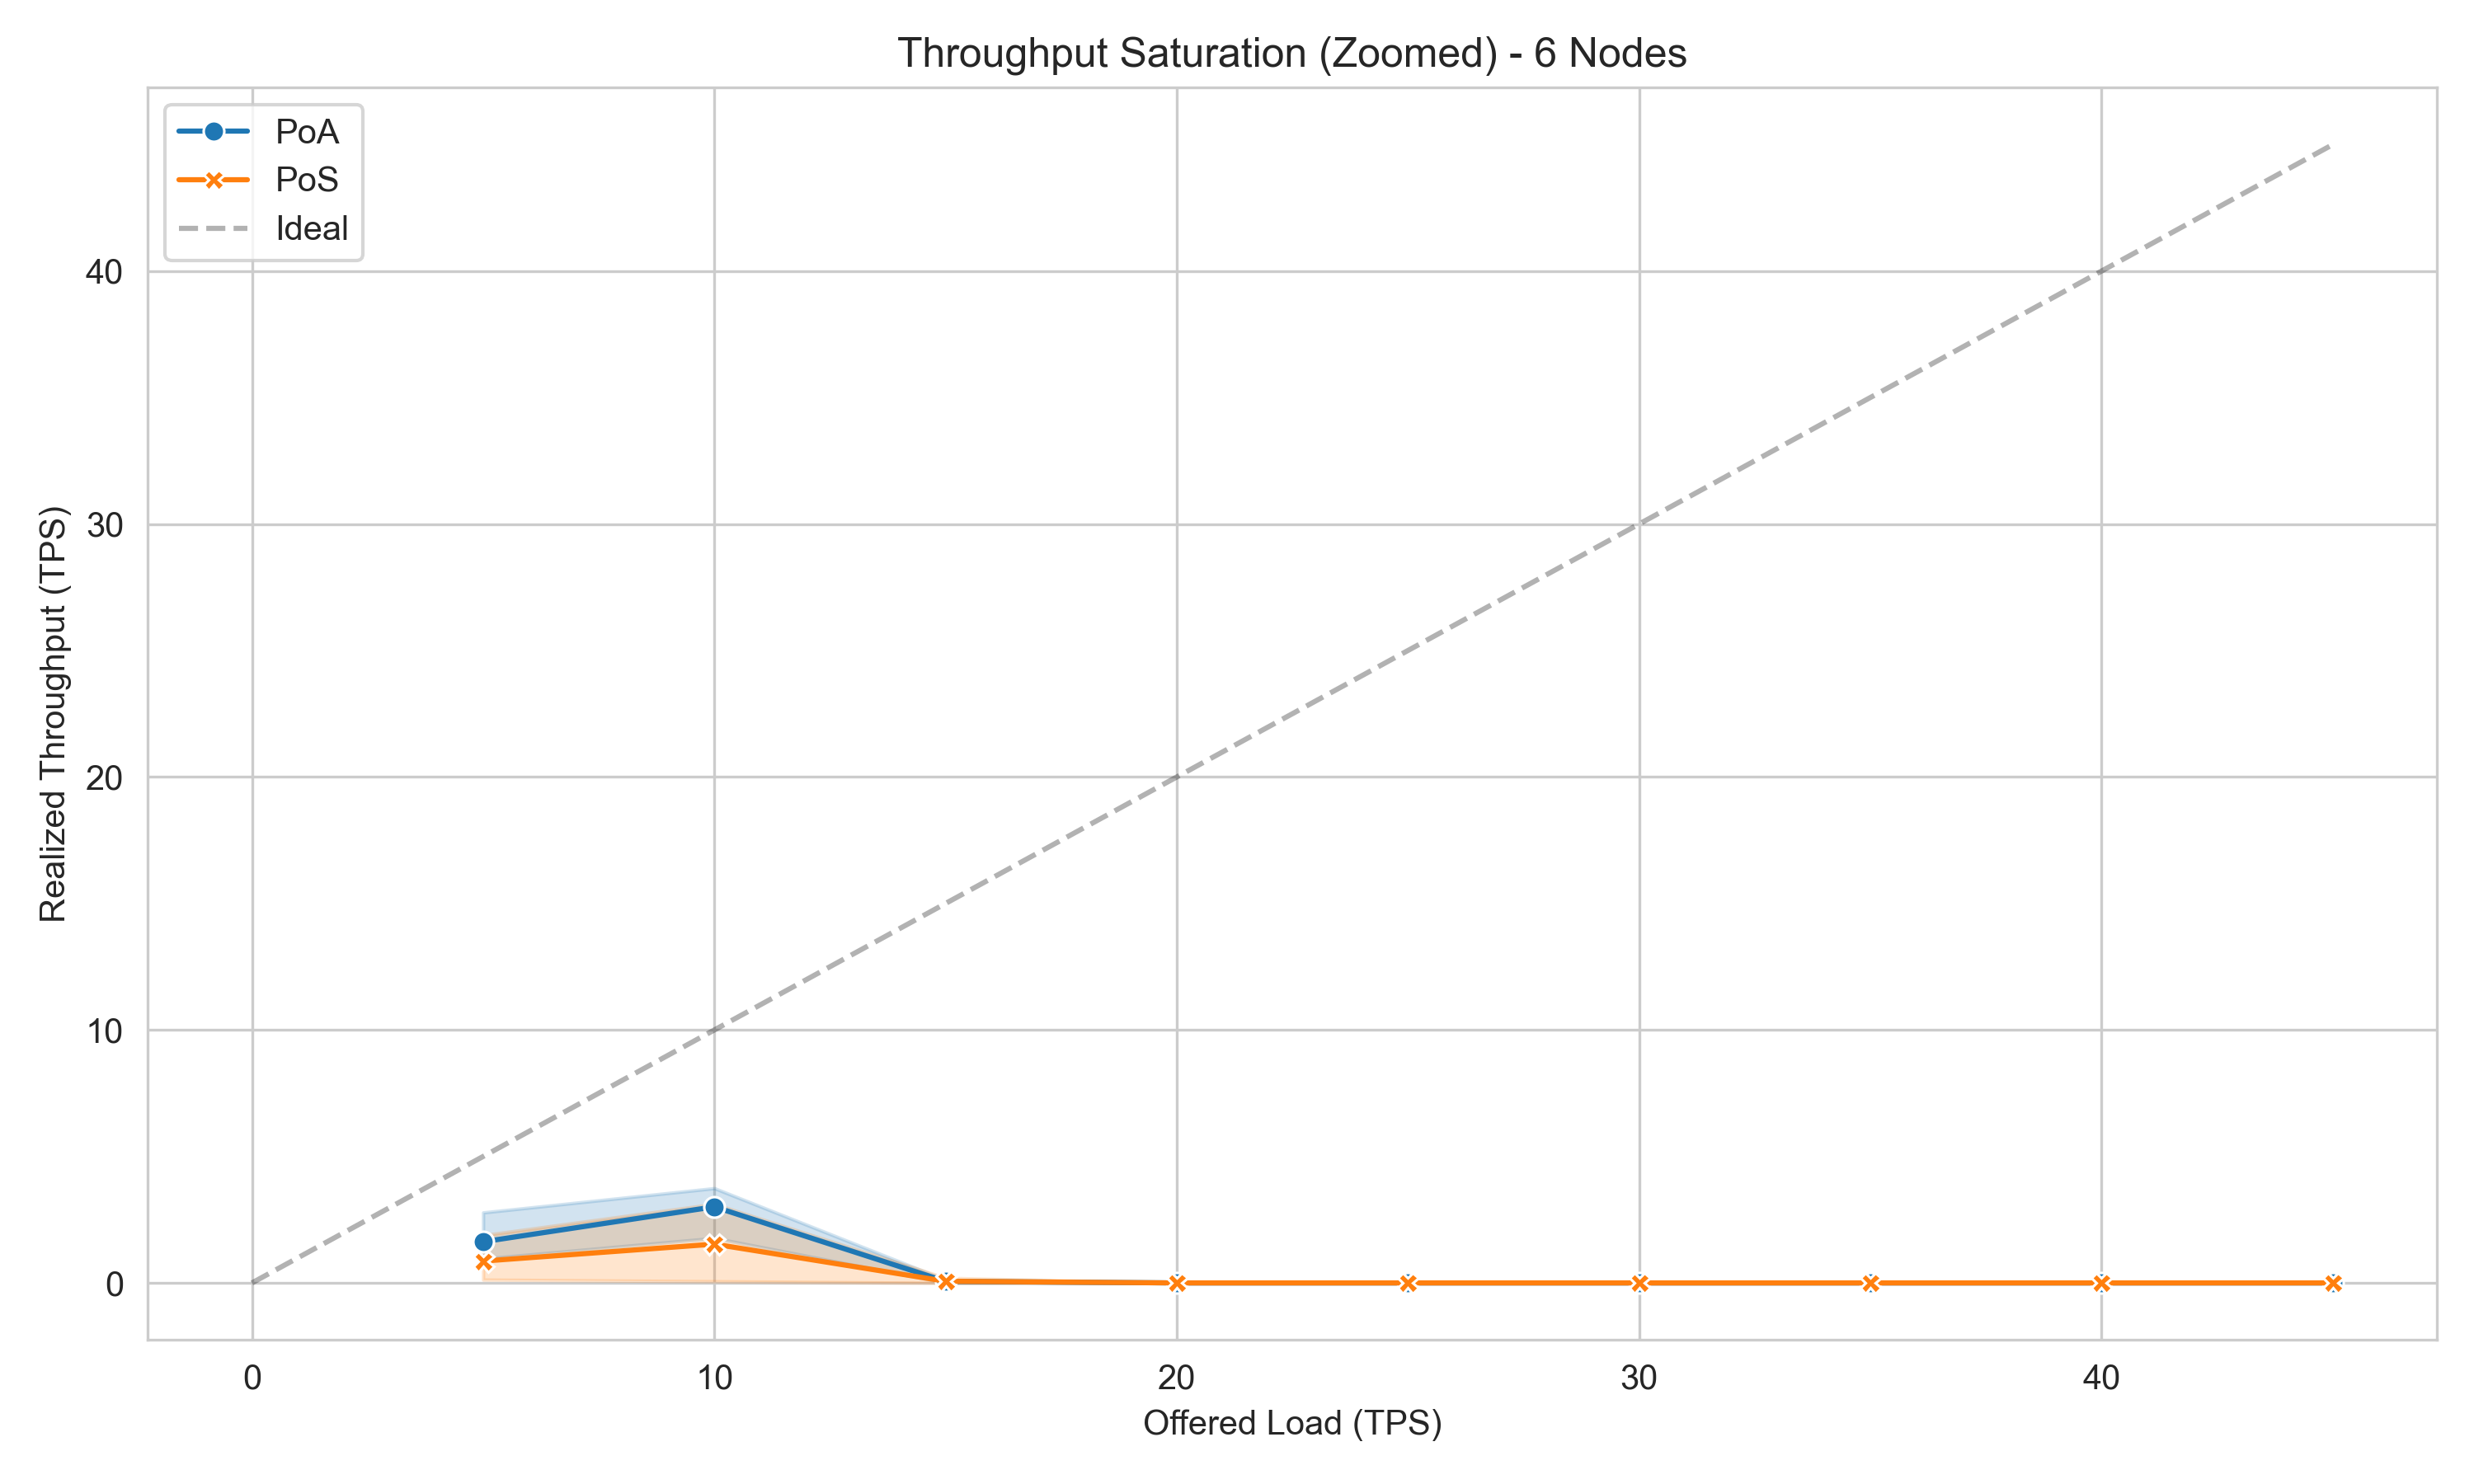
\includegraphics[width=0.9\textwidth]{images/throughput_curve_zoomed_6_Nodes.png}
    \caption{Kurva Throughput pada Topologi 6 Node}
    \label{fig:throughput_curve_6}
\end{figure}

\begin{figure}[htbp]
    \centering
    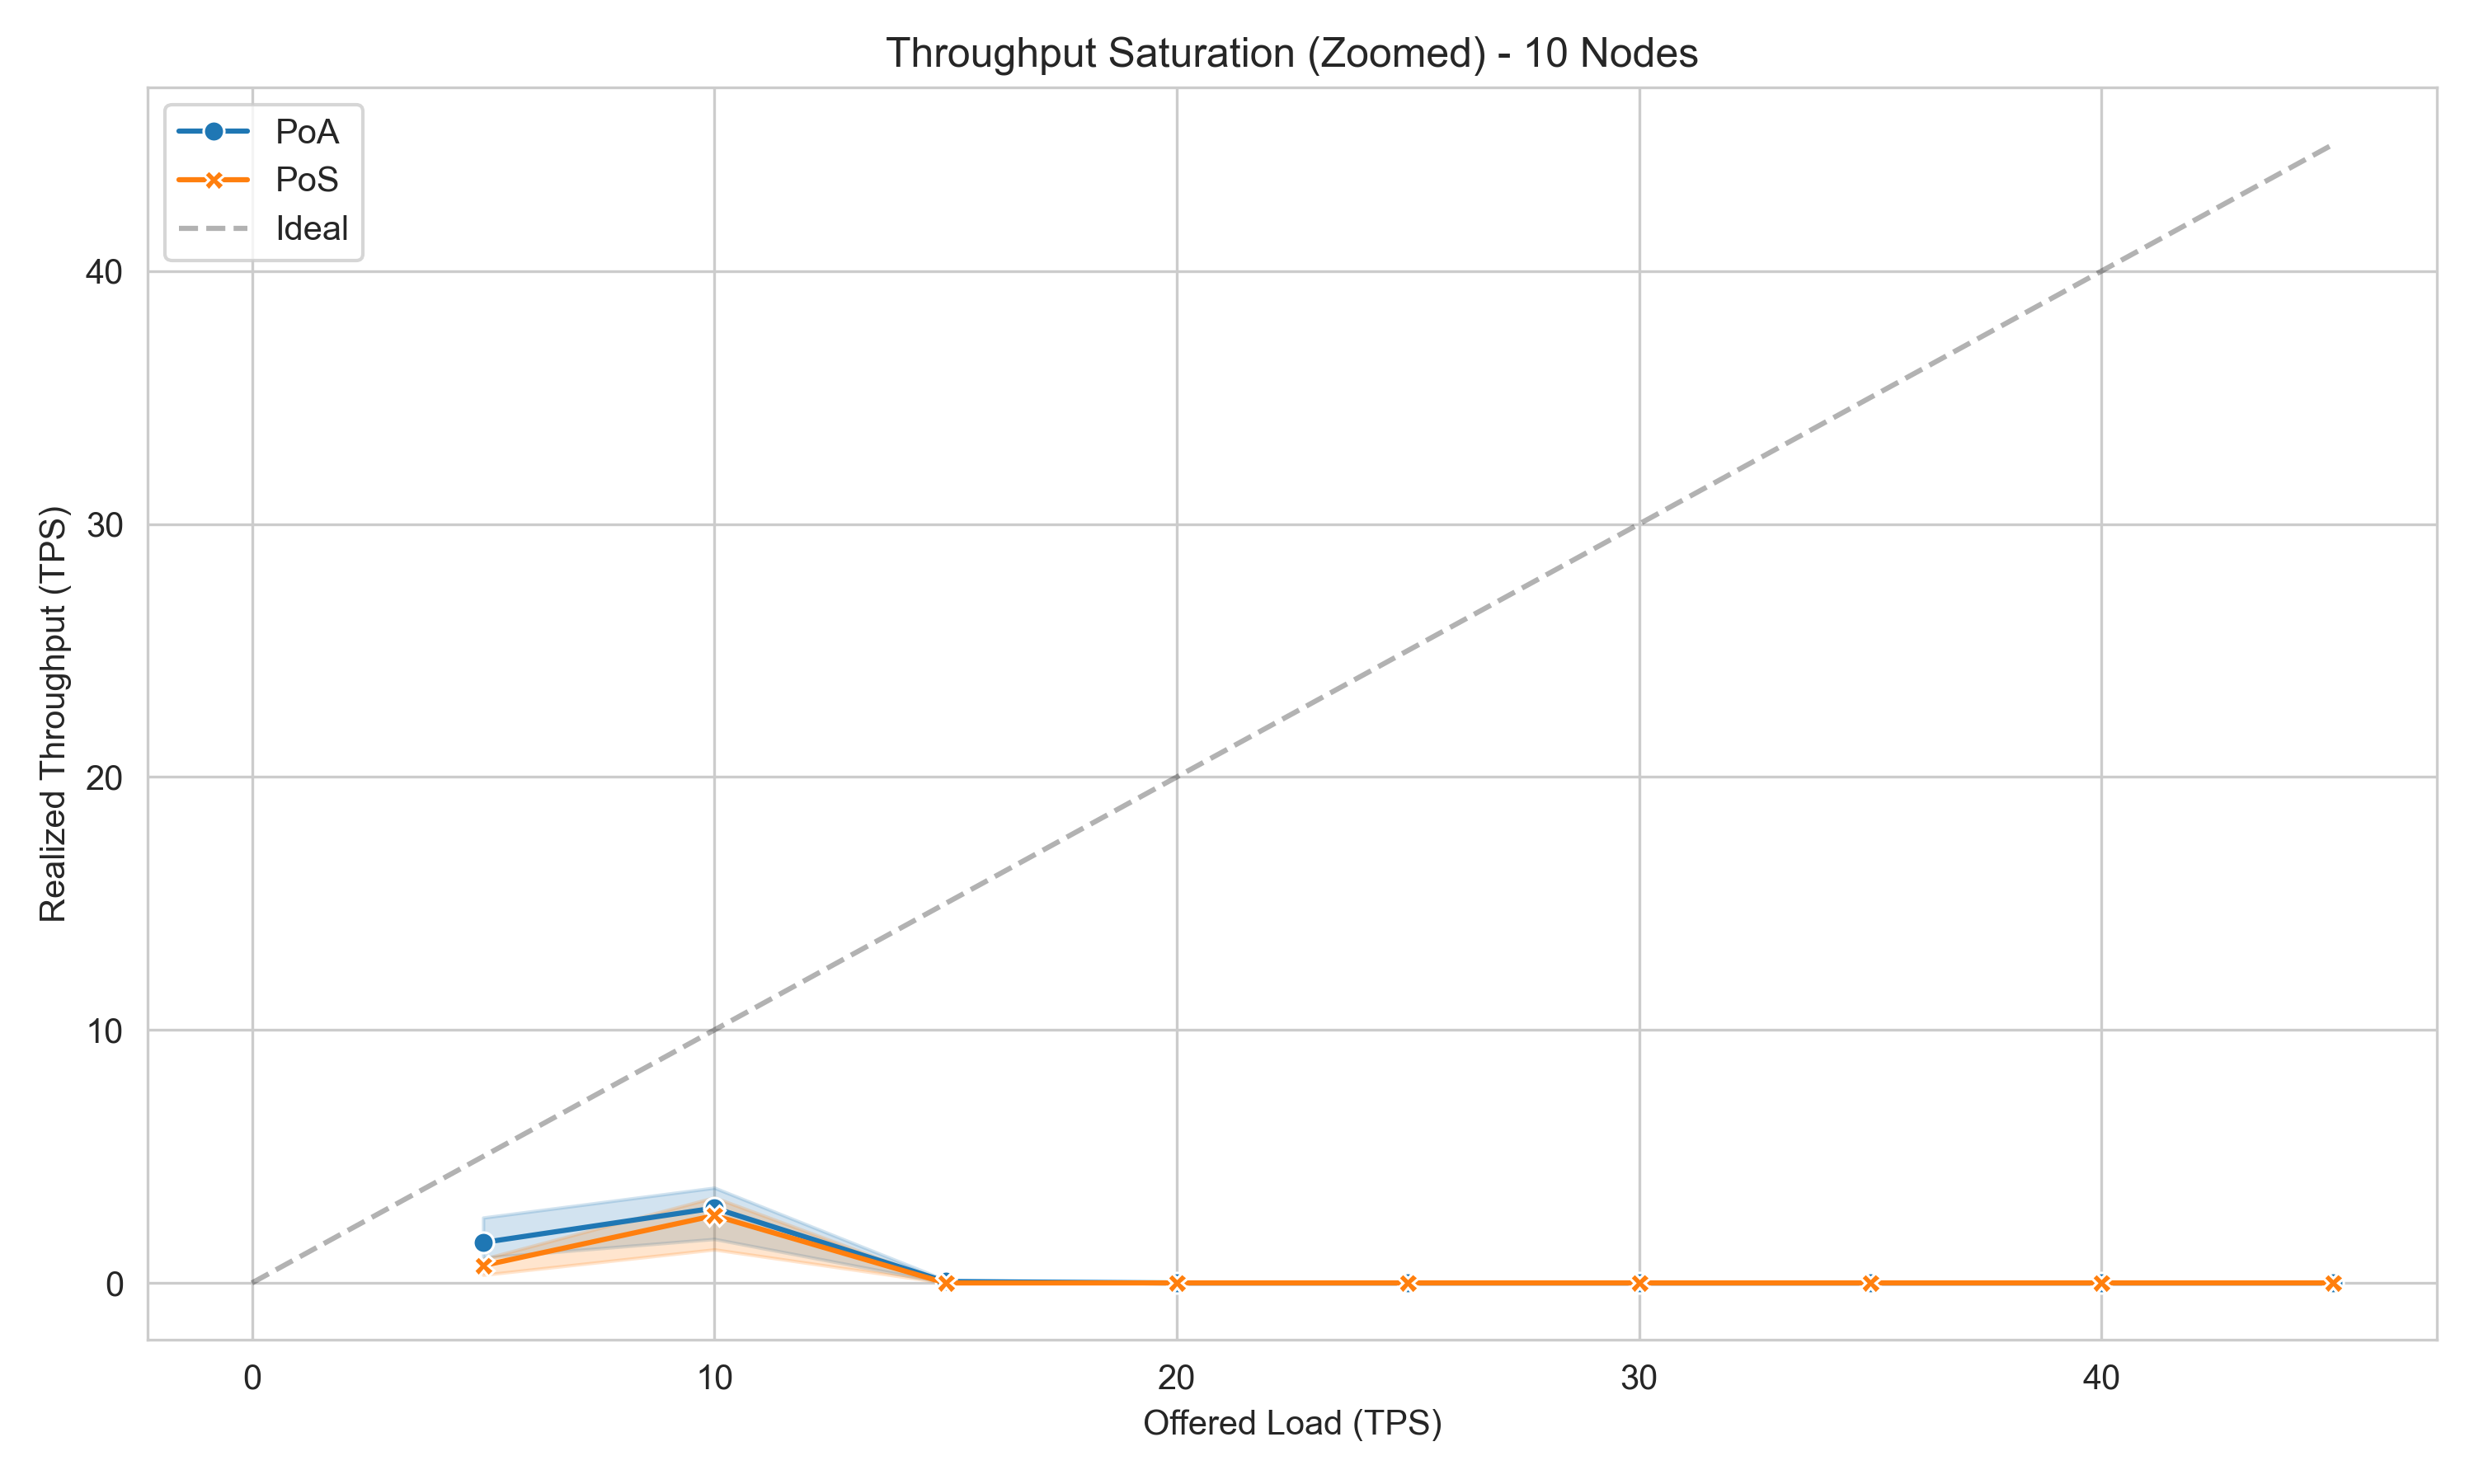
\includegraphics[width=0.9\textwidth]{images/throughput_curve_zoomed_10_Nodes.png}
    \caption{Kurva Throughput pada Topologi 10 Node}
    \label{fig:throughput_curve_10}
\end{figure}

\begin{figure}[htbp]
    \centering
    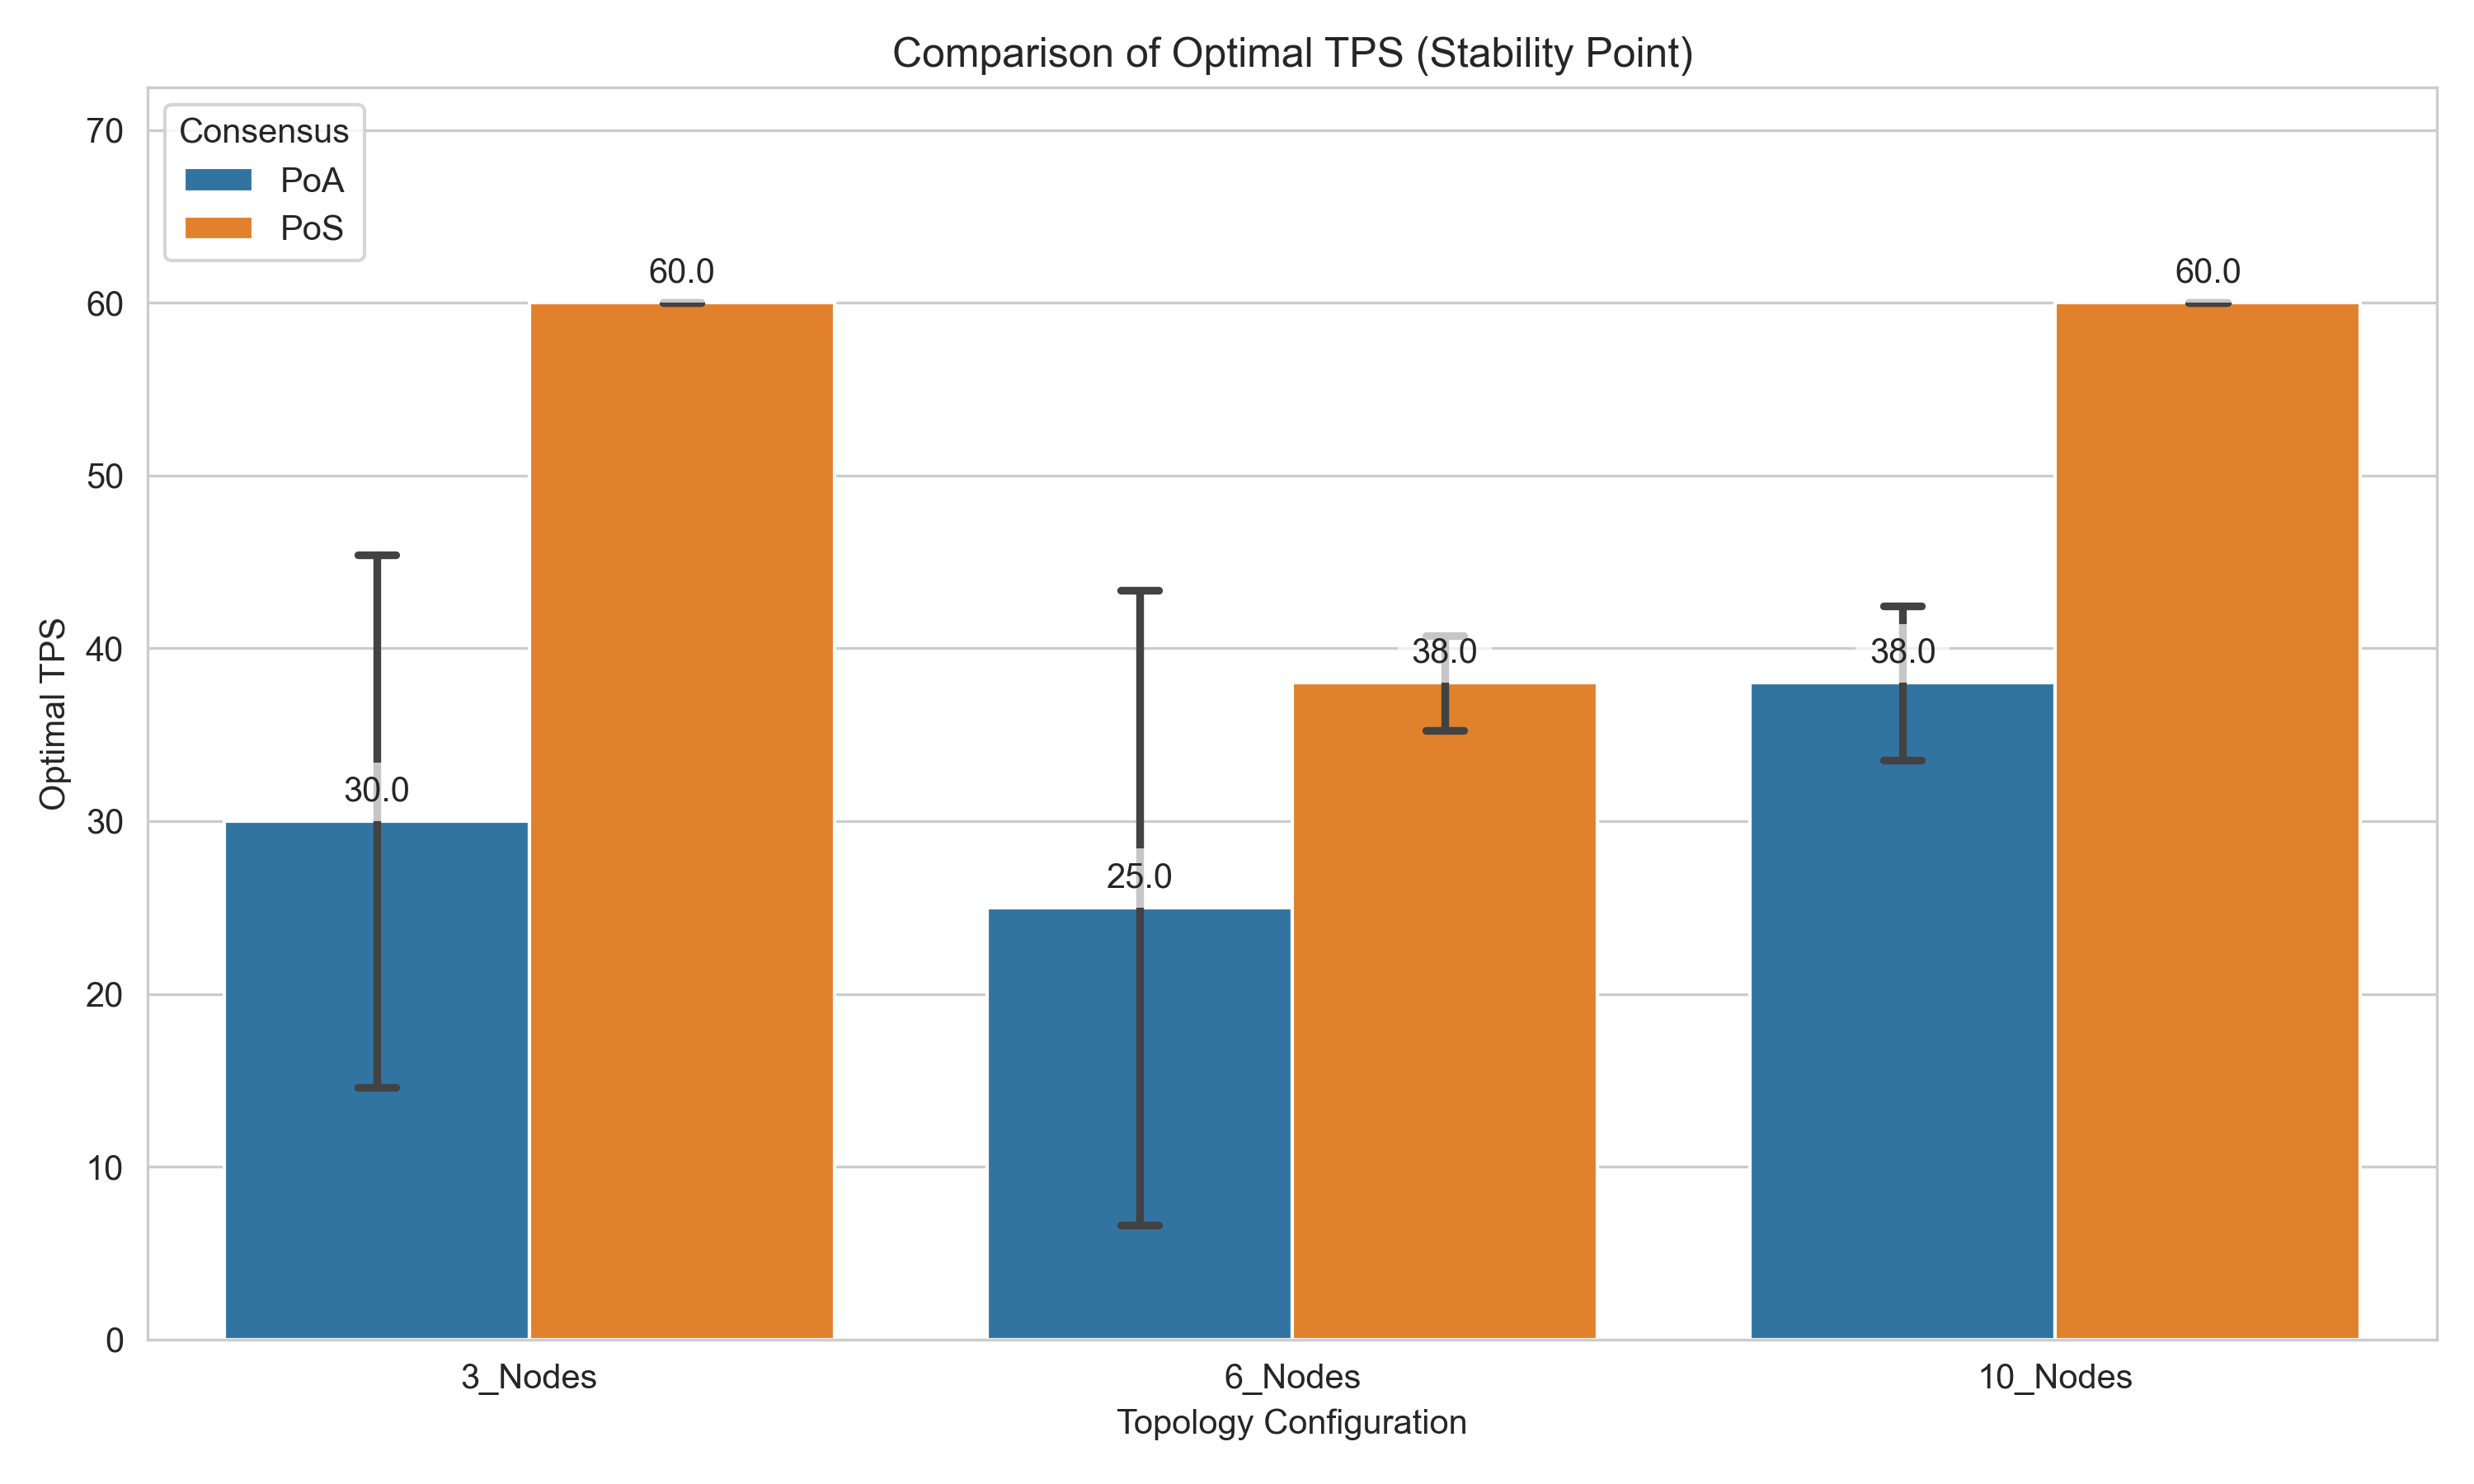
\includegraphics[width=0.9\textwidth]{images/optimal_tps_comparison.png}
    \caption{Perbandingan Optimal TPS}
    \label{fig:optimal_tps}
\end{figure}

\subsection{Latensi Transaksi}

Pengukuran latensi dilakukan pada kondisi \textit{steady-state} untuk melihat responsivitas jaringan. Grafik \textit{Latency Trade-off} pada Gambar \ref{fig:latency_tradeoff} hingga Gambar \ref{fig:latency_tradeoff_10} memperlihatkan pola "Hockey Stick", di mana latensi stabil pada beban rendah namun melonjak drastis saat jaringan mencapai saturasi.

Analisis lebih detail dari grafik tersebut menunjukkan:
\begin{itemize}
    \item \textbf{Baseline Latency}: Pada beban rendah ($<15$ TPS), PoA secara konsisten mencatat latensi rata-rata 4--5 detik (sesuai interval blok 5 detik), sedangkan PoS berkisar 7--8 detik. Ini menunjukkan PoA lebih responsif untuk beban ringan.
    \item \textbf{Latency Under Load}: Menariknya, saat beban mendekati titik jenuh, latensi PoS meningkat lebih tajam dibandingkan PoA. Gambar \ref{fig:latency_absolute} memperlihatkan perbandingan absolut ini, di mana PoA mempertahankan profil latensi yang lebih rendah dan terprediksi di hampir seluruh spektrum pengujian.
\end{itemize}

\begin{figure}[htbp]
    \centering
    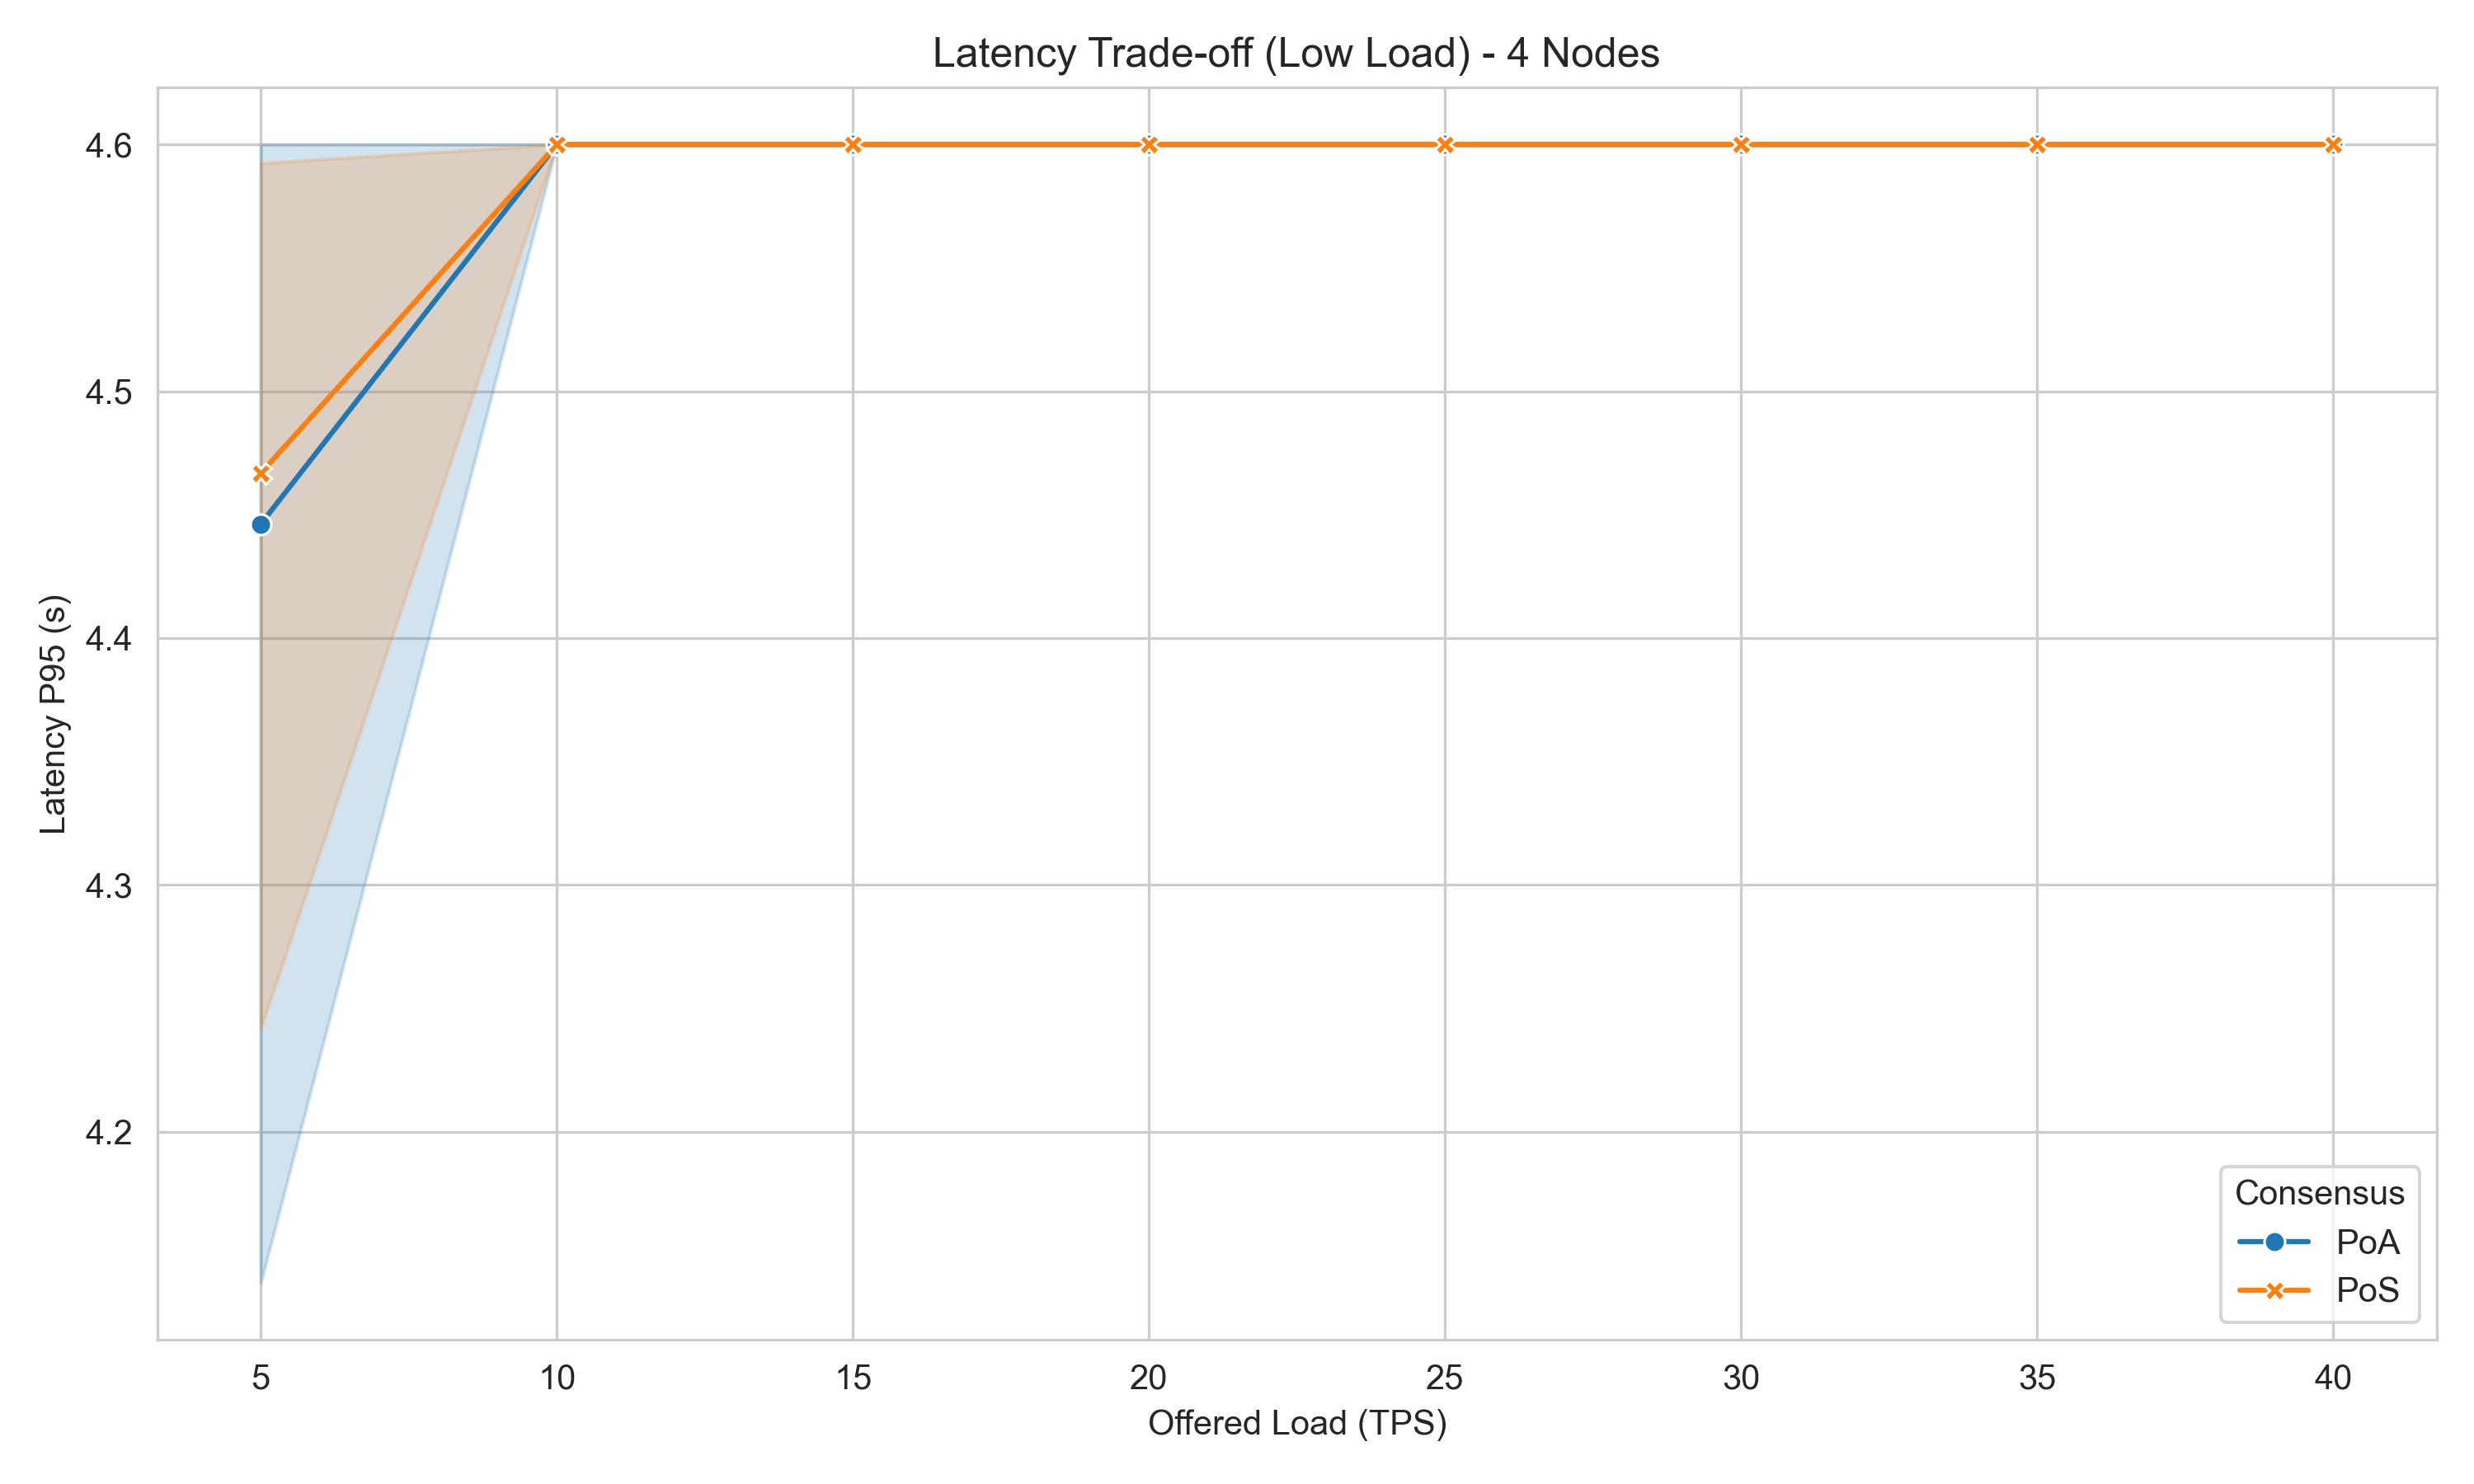
\includegraphics[width=0.9\textwidth]{images/latency_tradeoff_lowload_4_Nodes.png}
    \caption{Latency Trade-off pada Topologi 4 Node}
    \label{fig:latency_tradeoff}
\end{figure}

\begin{figure}[htbp]
    \centering
    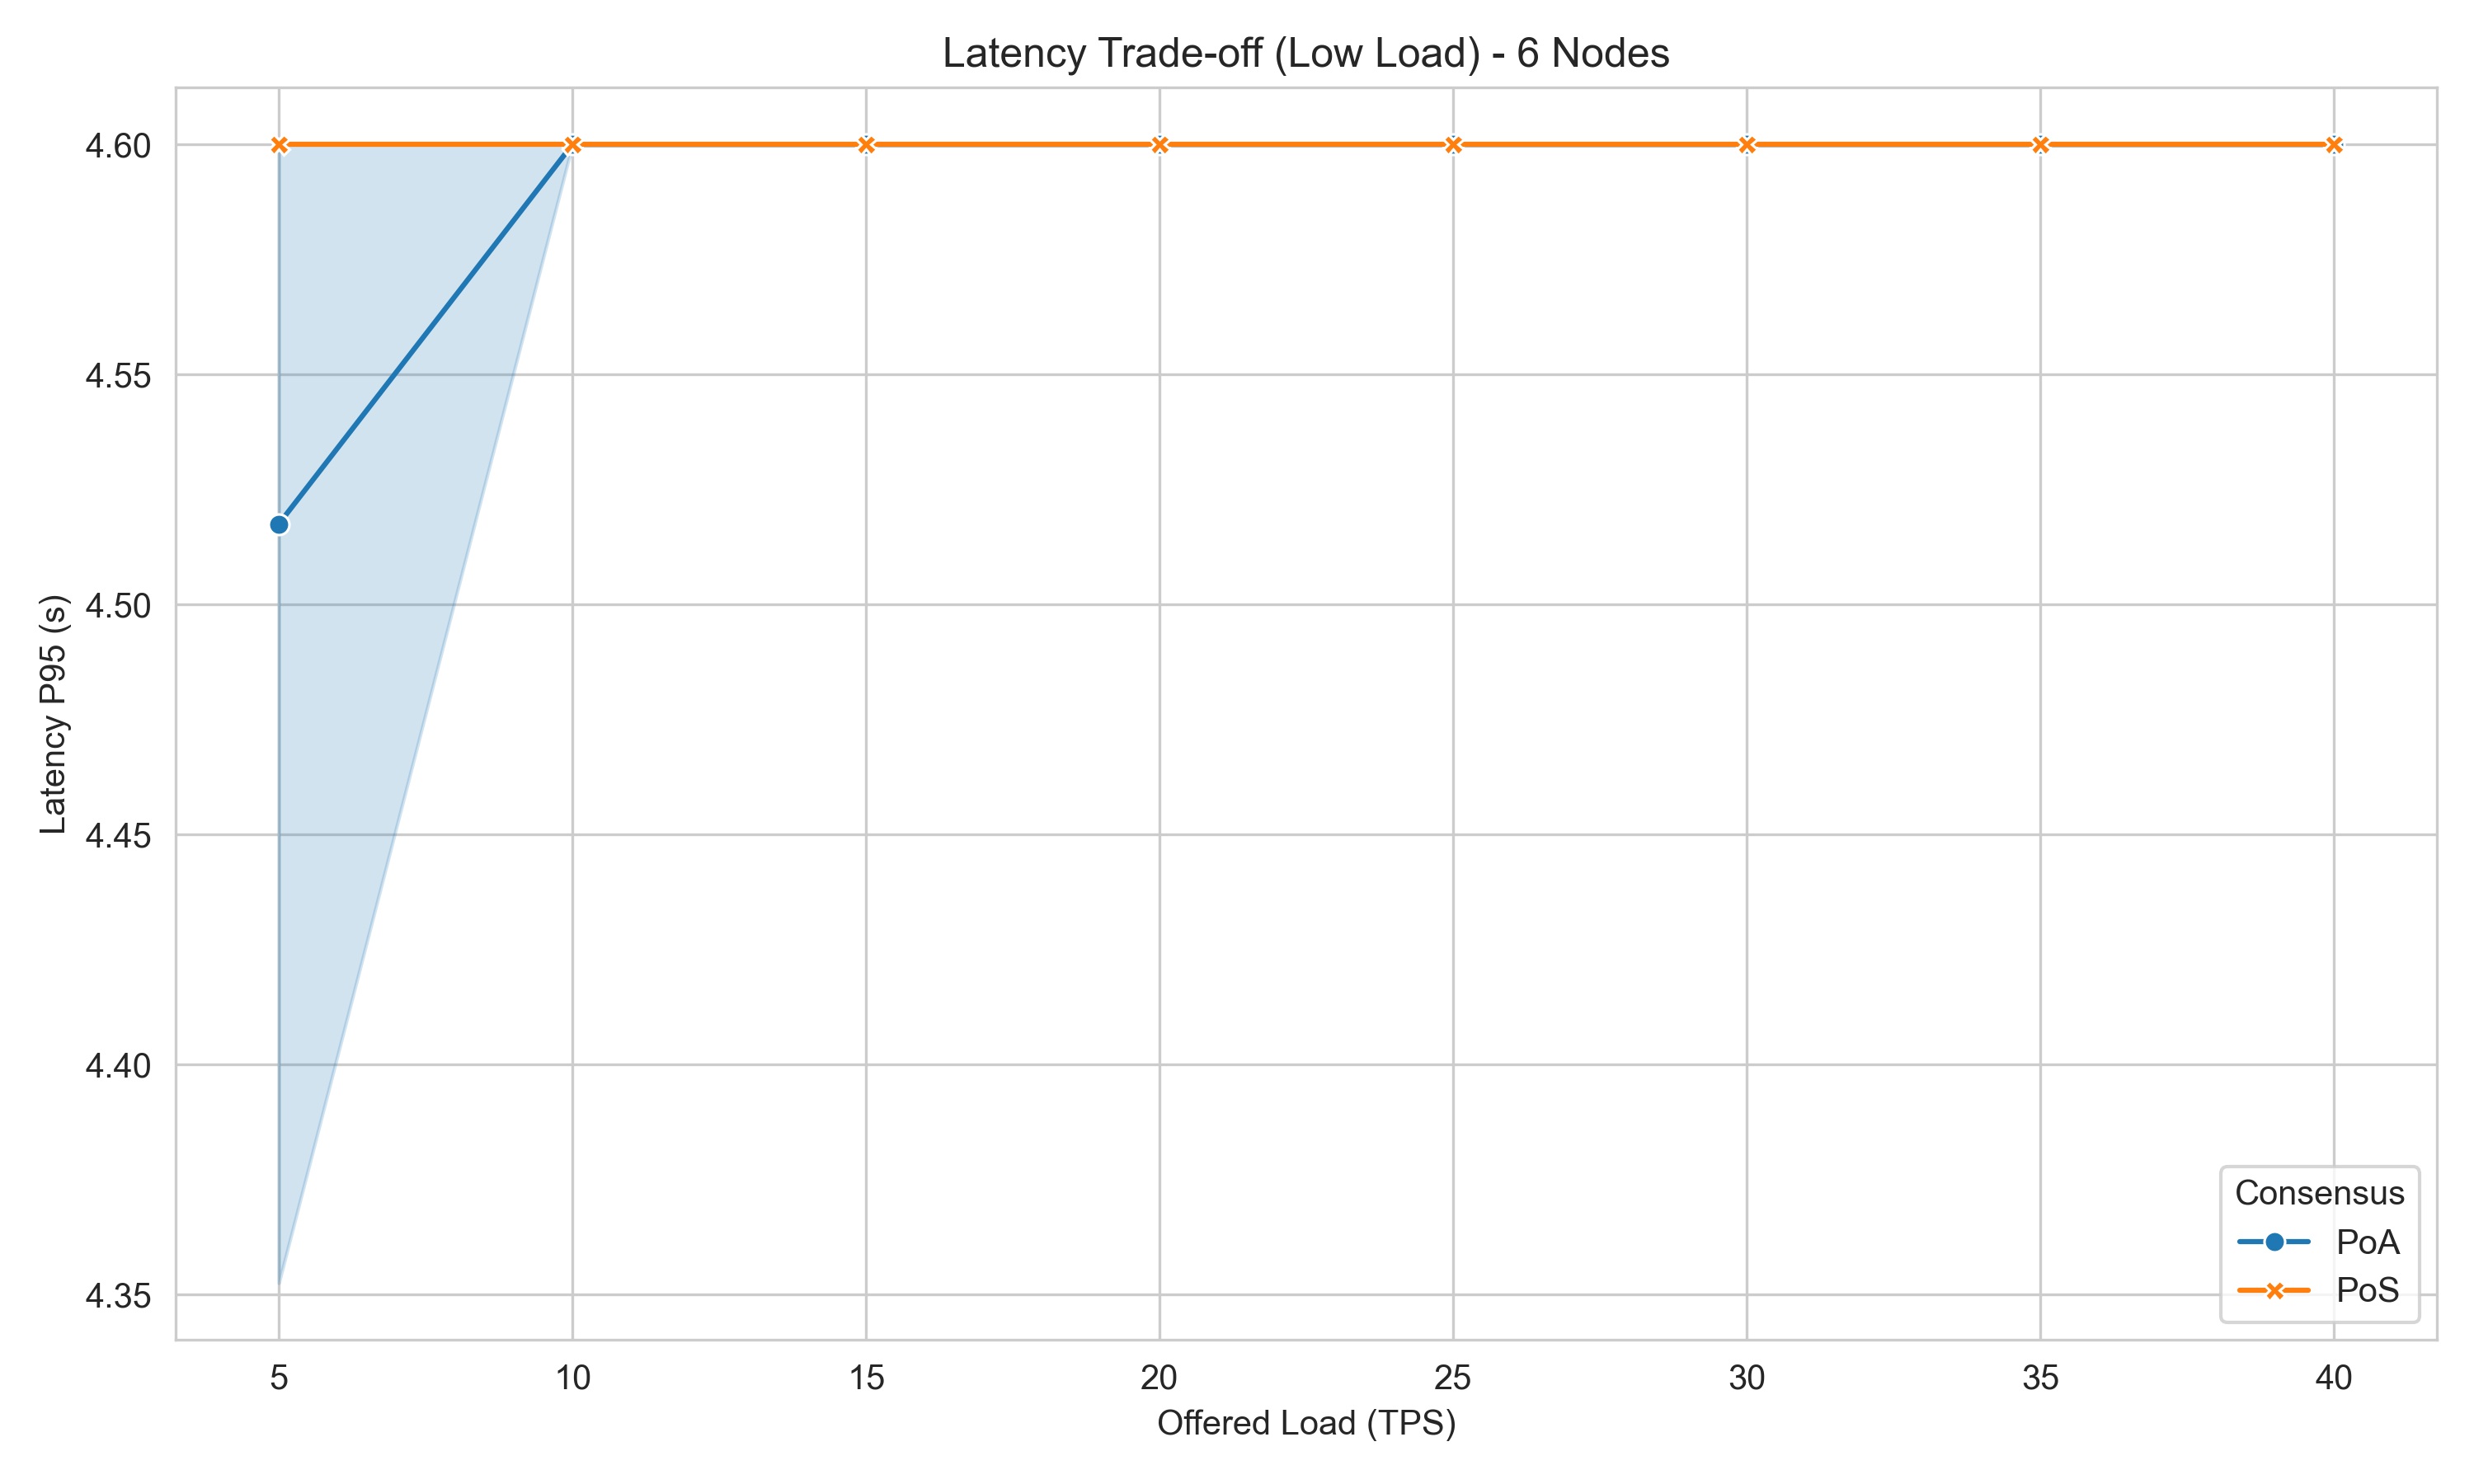
\includegraphics[width=0.9\textwidth]{images/latency_tradeoff_lowload_6_Nodes.png}
    \caption{Latency Trade-off pada Topologi 6 Node}
    \label{fig:latency_tradeoff_6}
\end{figure}

\begin{figure}[htbp]
    \centering
    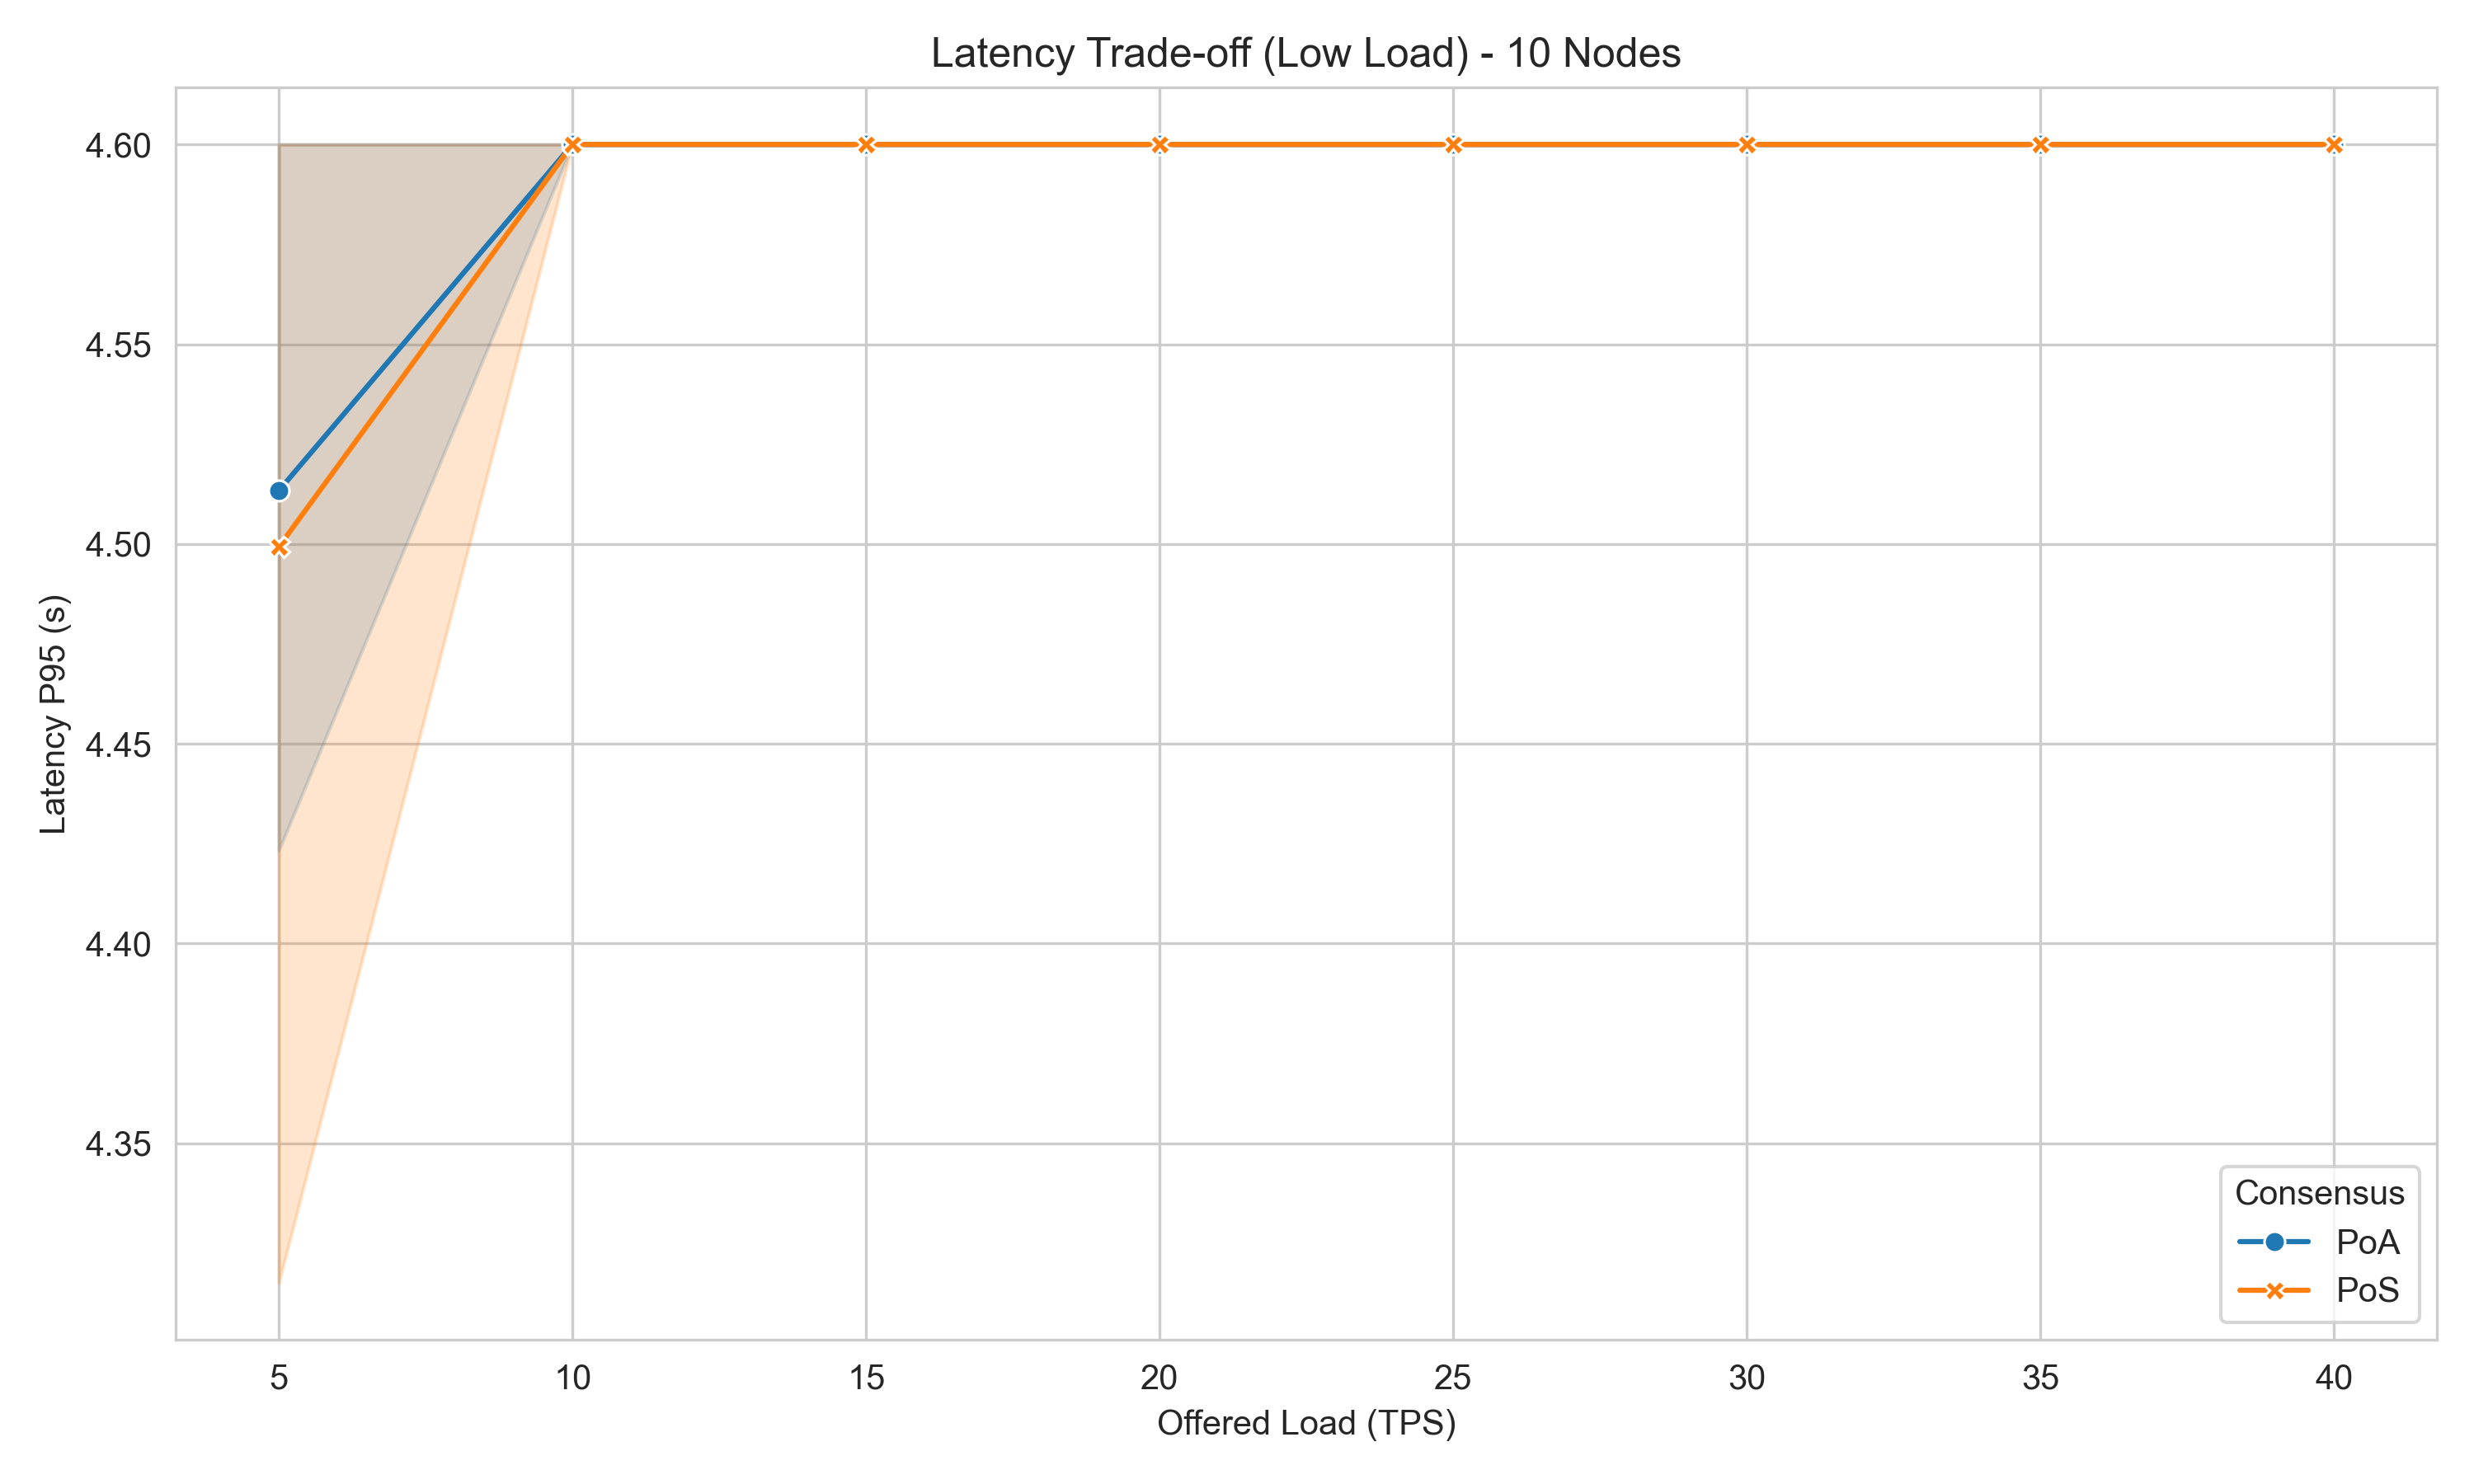
\includegraphics[width=0.9\textwidth]{images/latency_tradeoff_lowload_10_Nodes.png}
    \caption{Latency Trade-off pada Topologi 10 Node}
    \label{fig:latency_tradeoff_10}
\end{figure}

\begin{figure}[htbp]
    \centering
    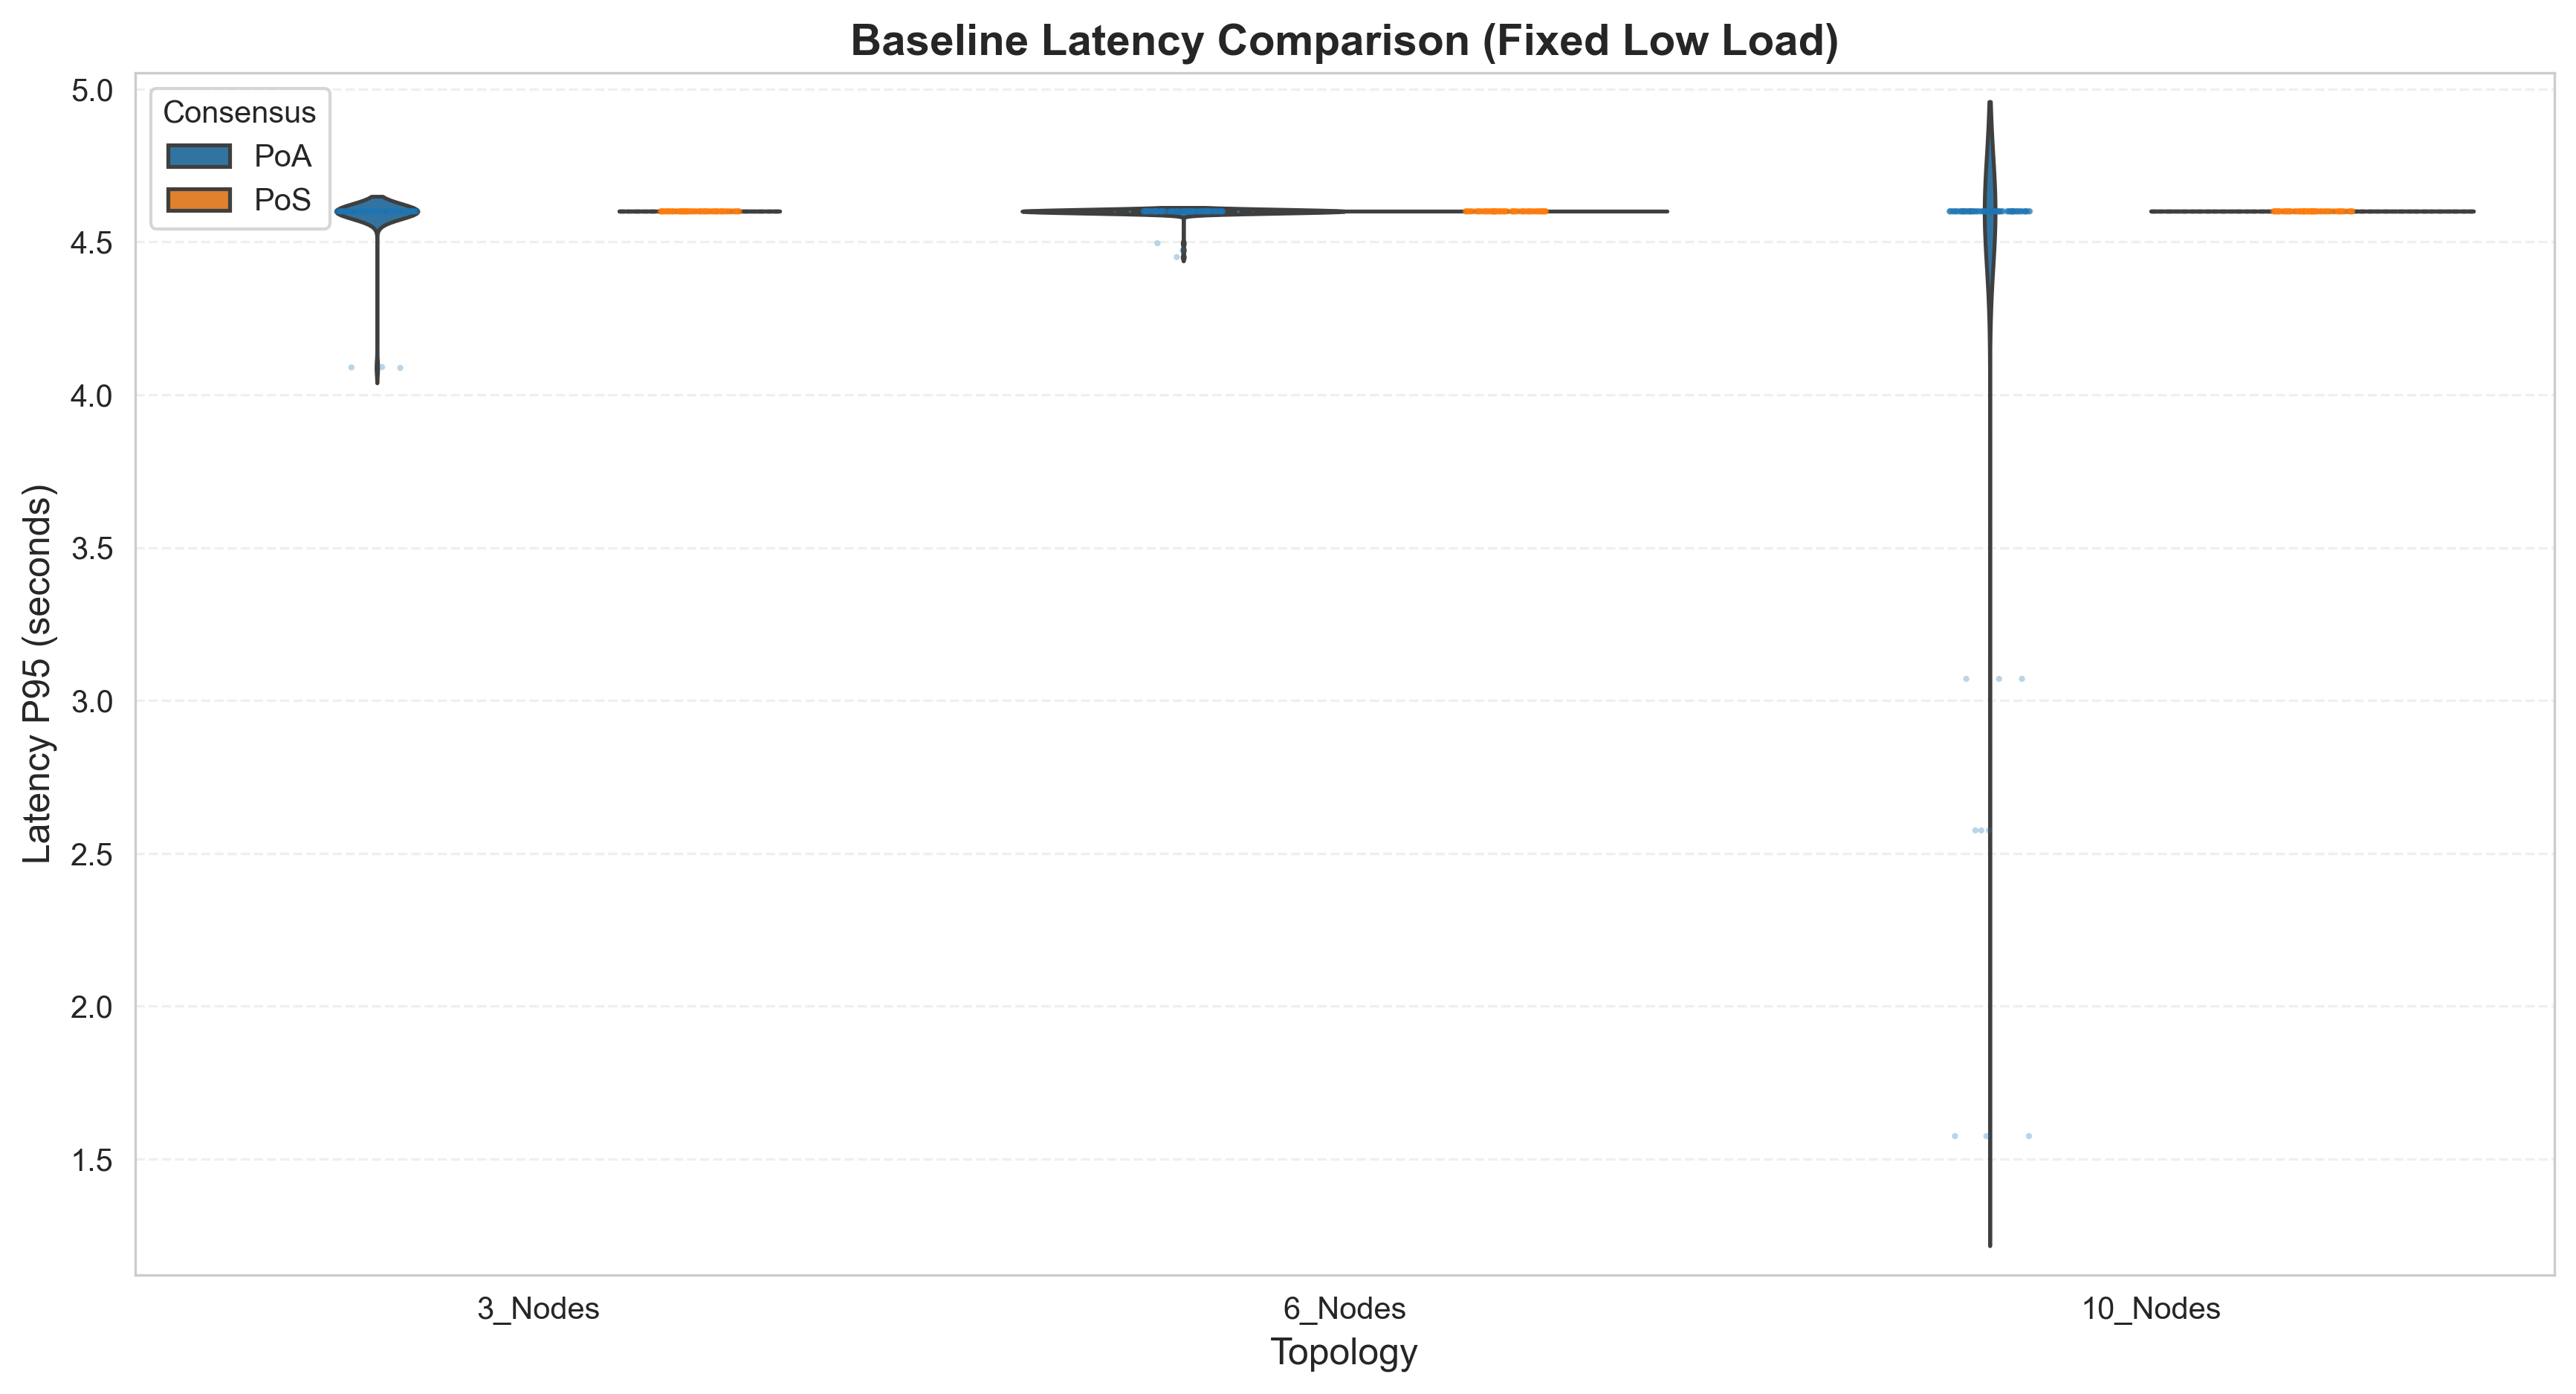
\includegraphics[width=0.9\textwidth]{images/latency_absolute_comparison.png}
    \caption{Perbandingan Latensi Absolut PoA vs PoS}
    \label{fig:latency_absolute}
\end{figure}

\subsection{Efisiensi Sumber Daya \& Skalabilitas}

Efisiensi penggunaan sumber daya prosesor divisualisasikan pada Gambar \ref{fig:efficiency_cpu}. Metrik "TPS per \% CPU" menunjukkan seberapa banyak transaksi yang dapat diproses untuk setiap persen daya CPU yang dikonsumsi.
Hasil pada Gambar \ref{fig:efficiency_cpu} memperlihatkan bahwa PoA jauh lebih efisien dibanding PoS. PoA mampu memproses lebih banyak transaksi dengan daya komputasi yang minimal, sedangkan PoS memiliki \textit{overhead} komputasi yang signifikan. Hal ini diperkuat dengan hasil uji \textit{CPU Stress} pada Gambar \ref{fig:cpu_stress}, di mana performa PoS menurun lebih drastis dibandingkan PoA saat sumber daya CPU dibatasi secara ekstrim.

Terkait skalabilitas klien (Gambar \ref{fig:scalability_client_4} hingga \ref{fig:scalability_client_10}), kedua konsensus mengalami degradasi performa total saat jumlah \textit{worker} dinaikkan dari 1 ke 5. Ini mengindikasikan adanya \textit{bottleneck} pada sisi klien Caliper atau antrian RPC node, bukan pada konsensus itu sendiri. Namun, pola penurunannya serupa untuk kedua mekanisme.

\begin{figure}[htbp]
    \centering
    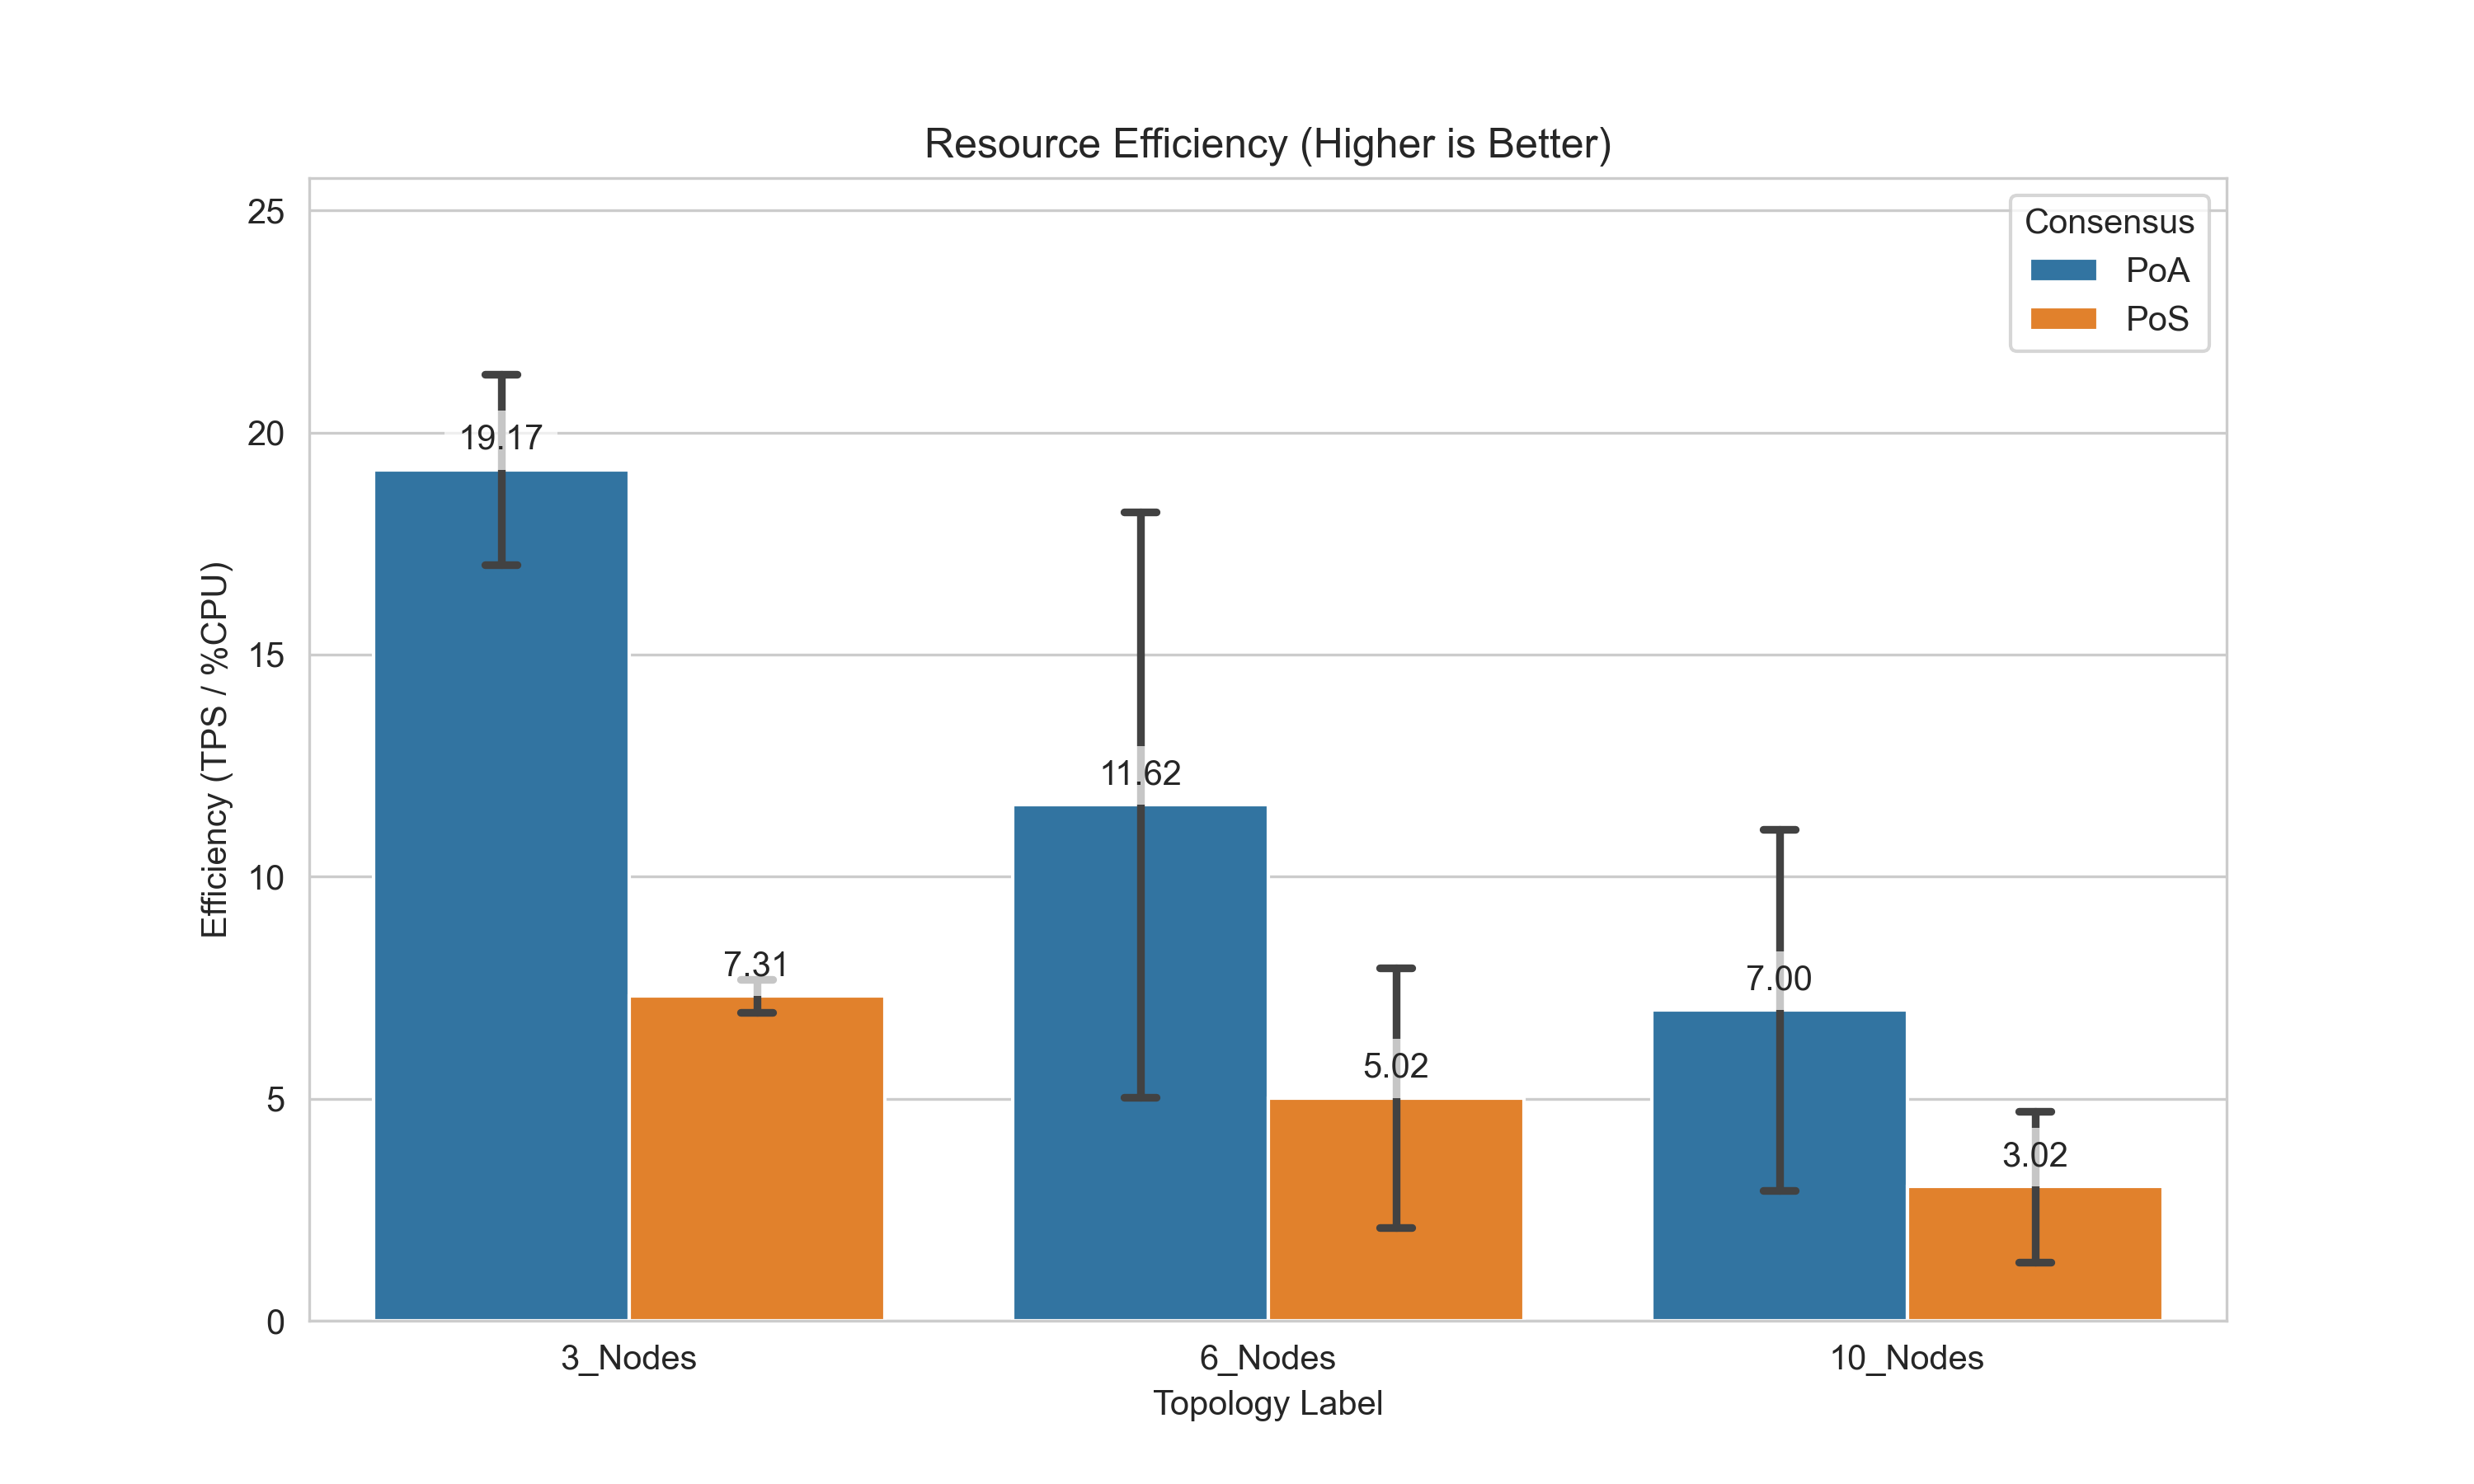
\includegraphics[width=0.9\textwidth]{images/efficiency_resource_cpu.png}
    \caption{Efisiensi Sumber Daya (TPS per \% CPU)}
    \label{fig:efficiency_cpu}
\end{figure}

\begin{figure}[htbp]
    \centering
    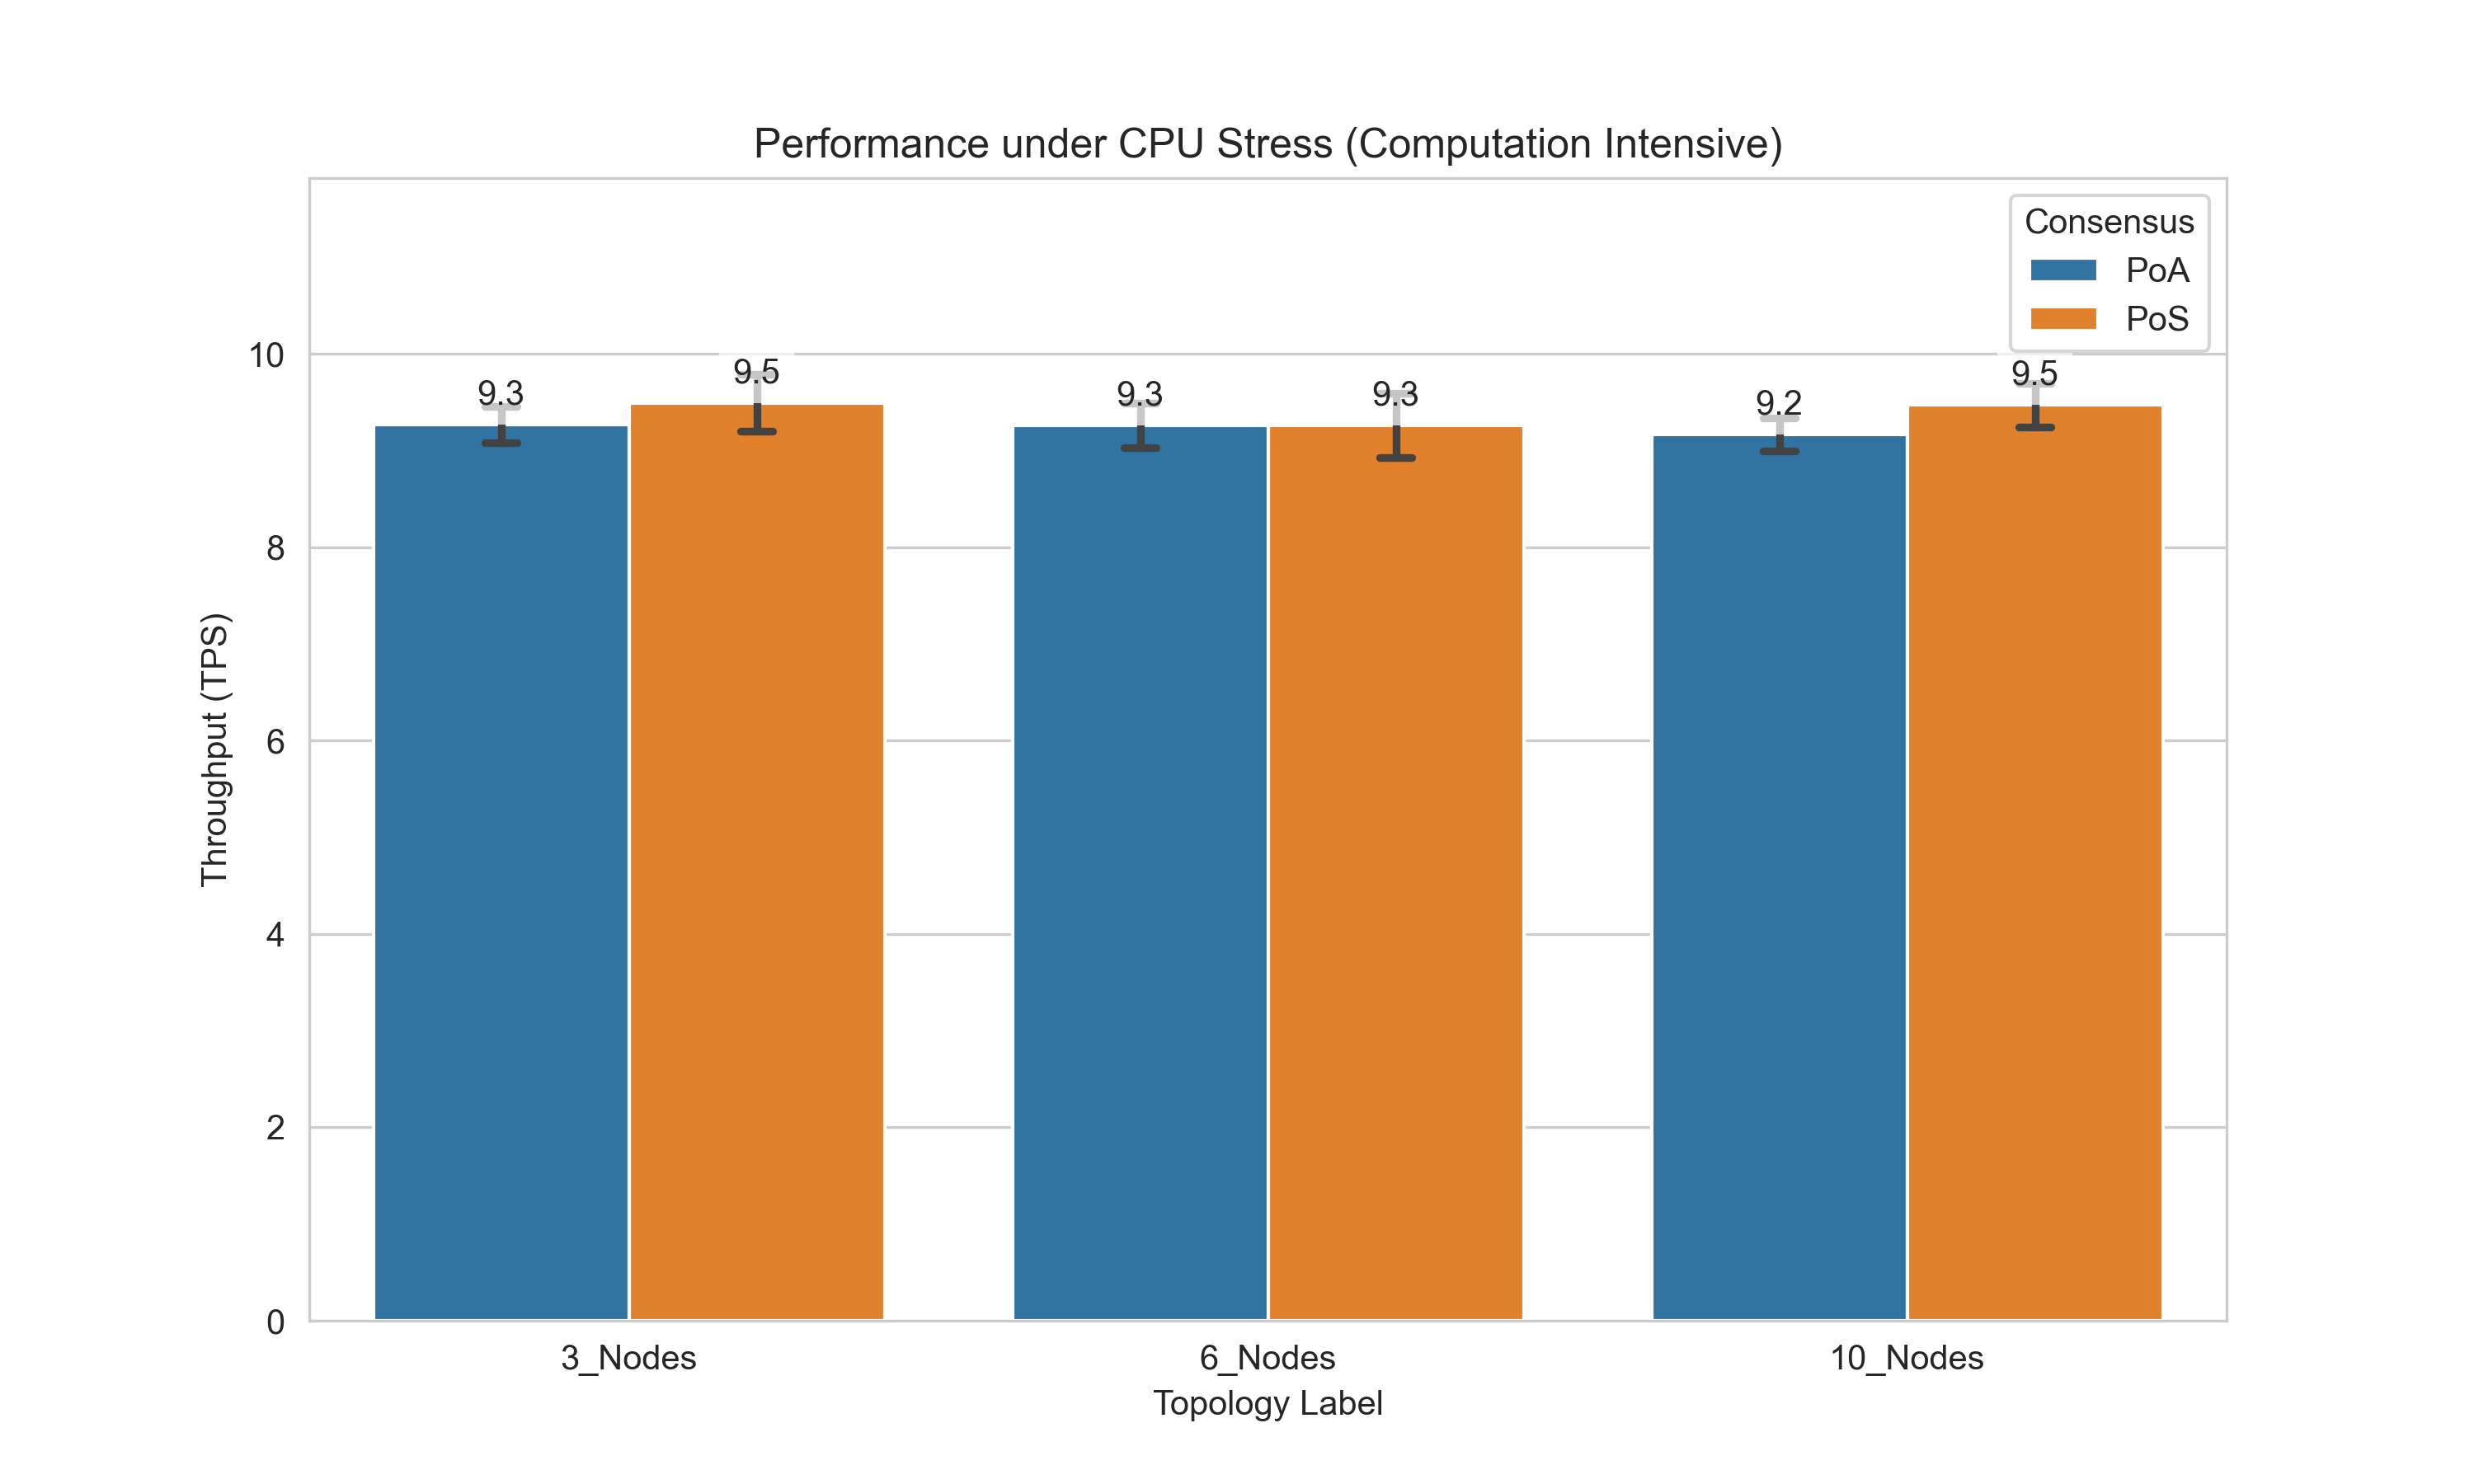
\includegraphics[width=0.9\textwidth]{images/cpu_stress_comparison.png}
    \caption{Perbandingan CPU Stress Test}
    \label{fig:cpu_stress}
\end{figure}

\begin{figure}[htbp]
    \centering
    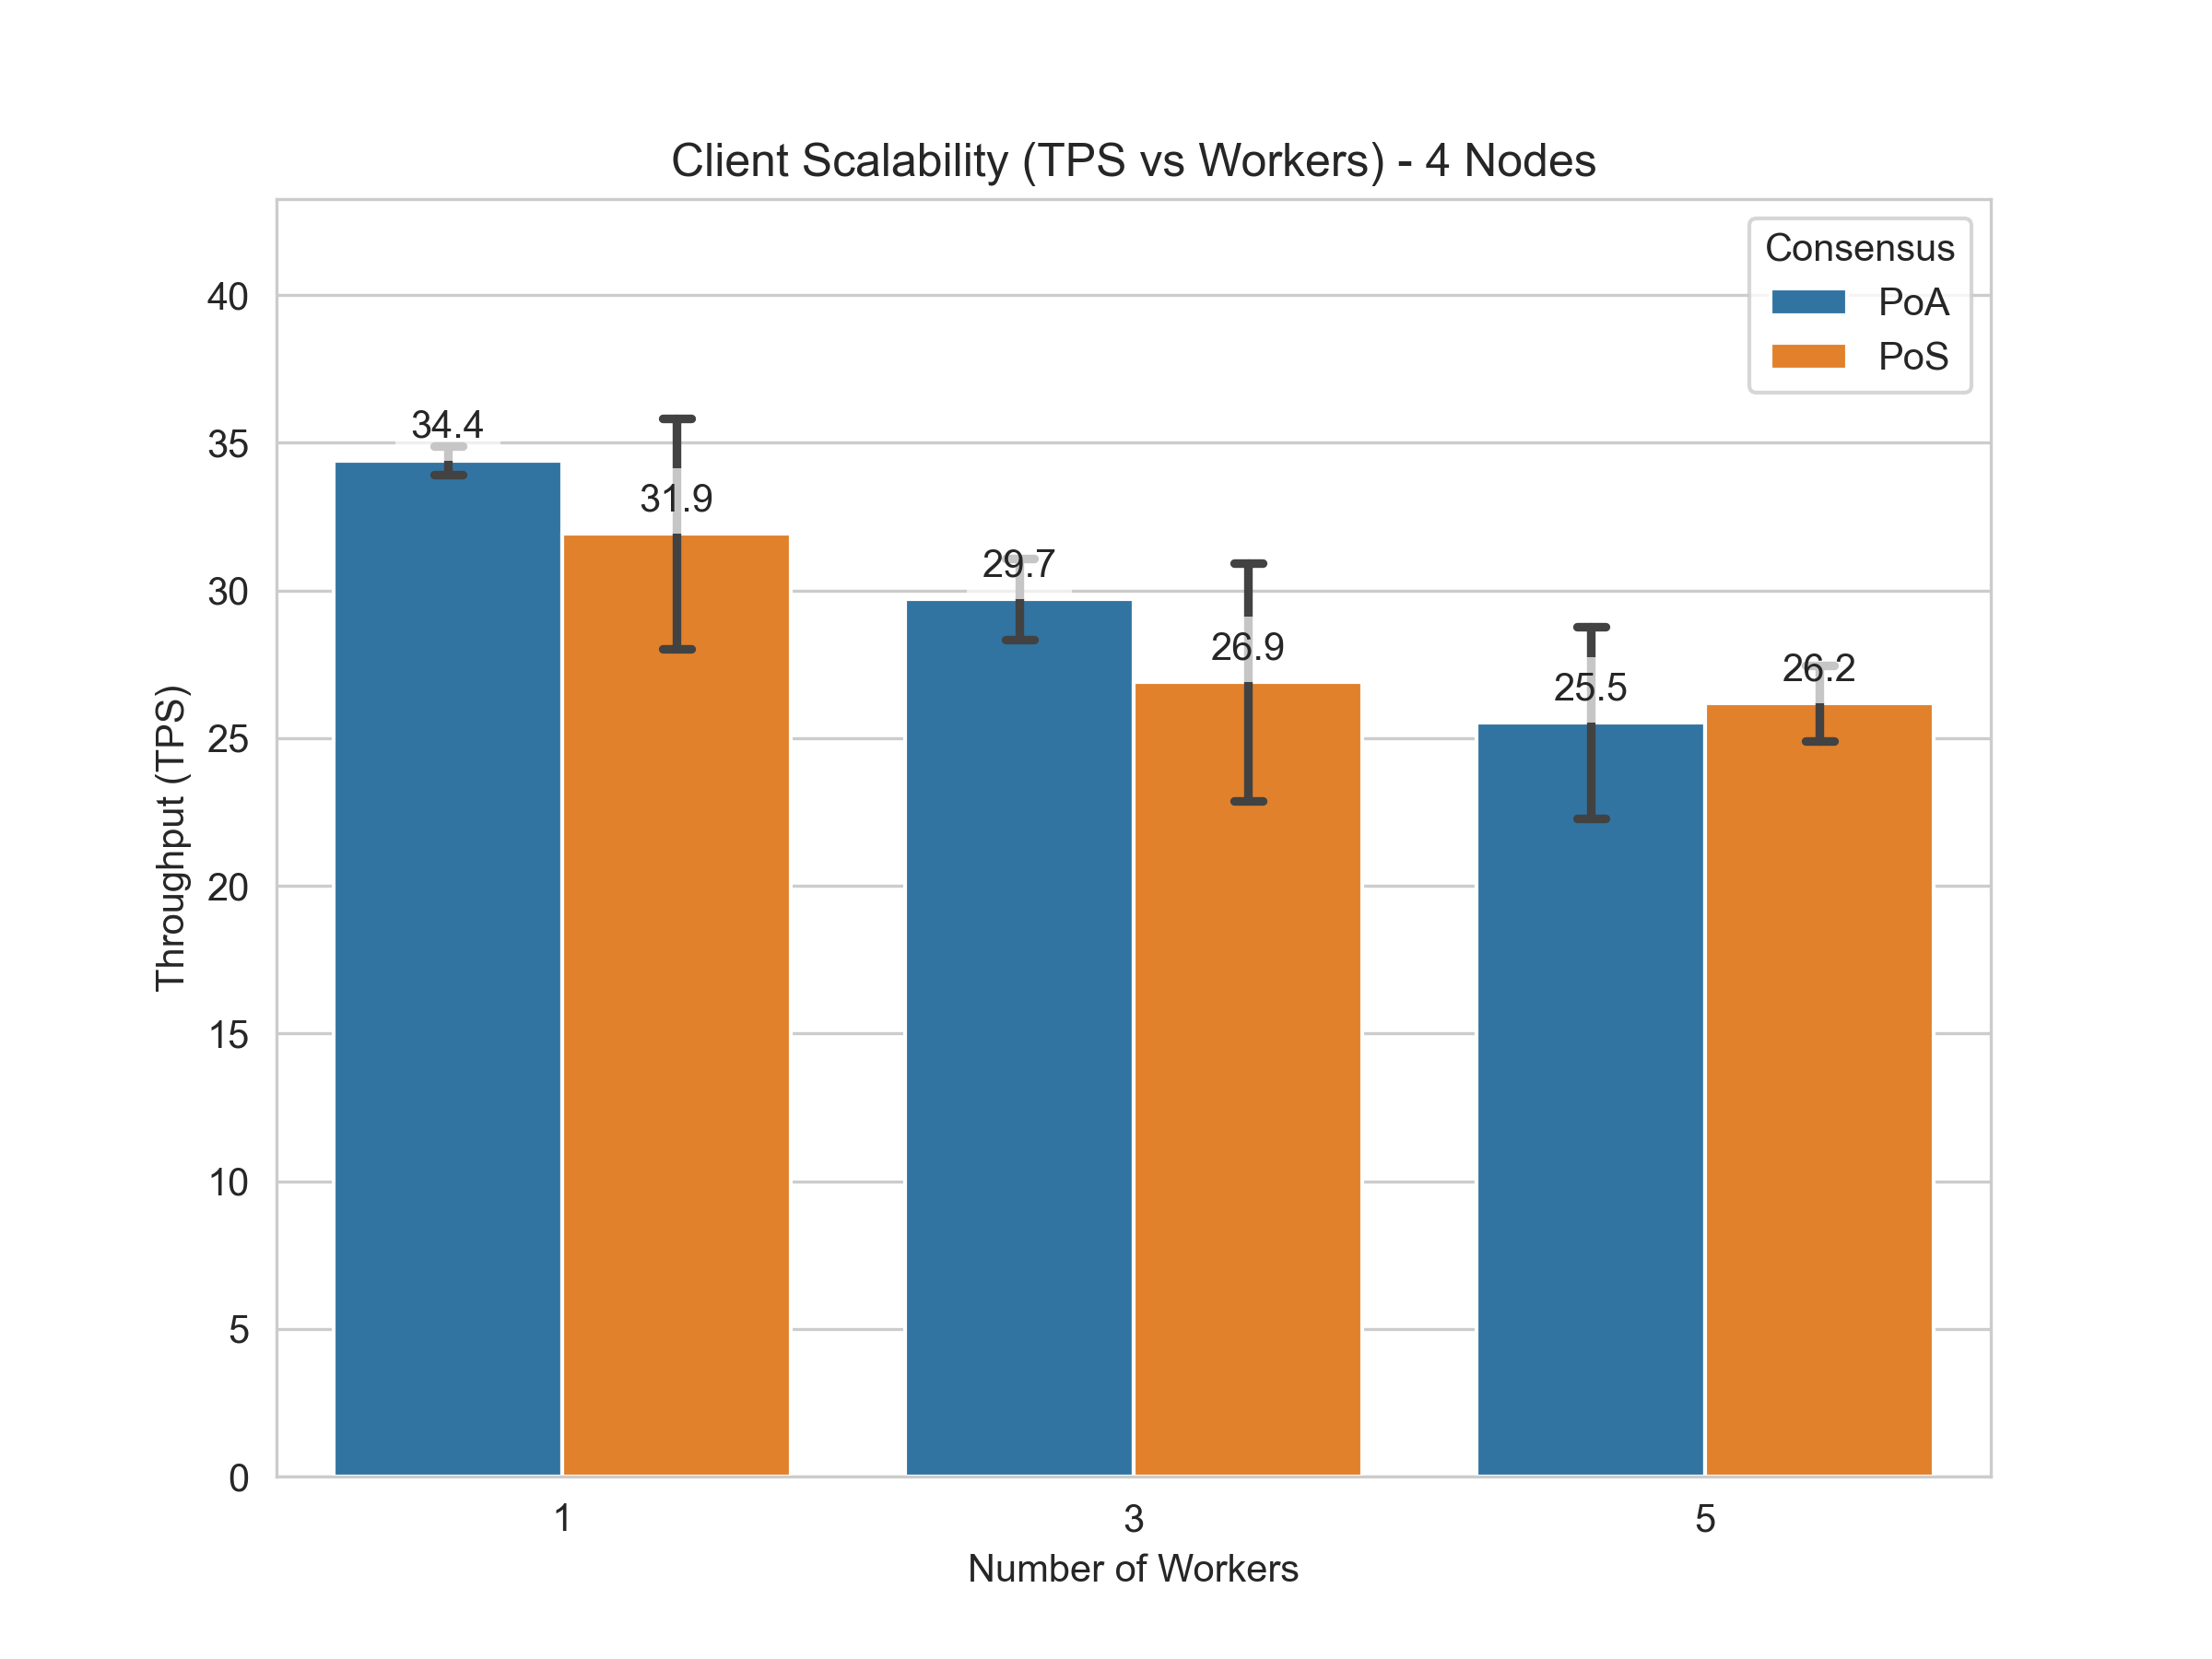
\includegraphics[width=0.9\textwidth]{images/scalability_client_tps_4_Nodes.png}
    \caption{Skalabilitas Klien pada Topologi 4 Node}
    \label{fig:scalability_client_4}
\end{figure}

\begin{figure}[htbp]
    \centering
    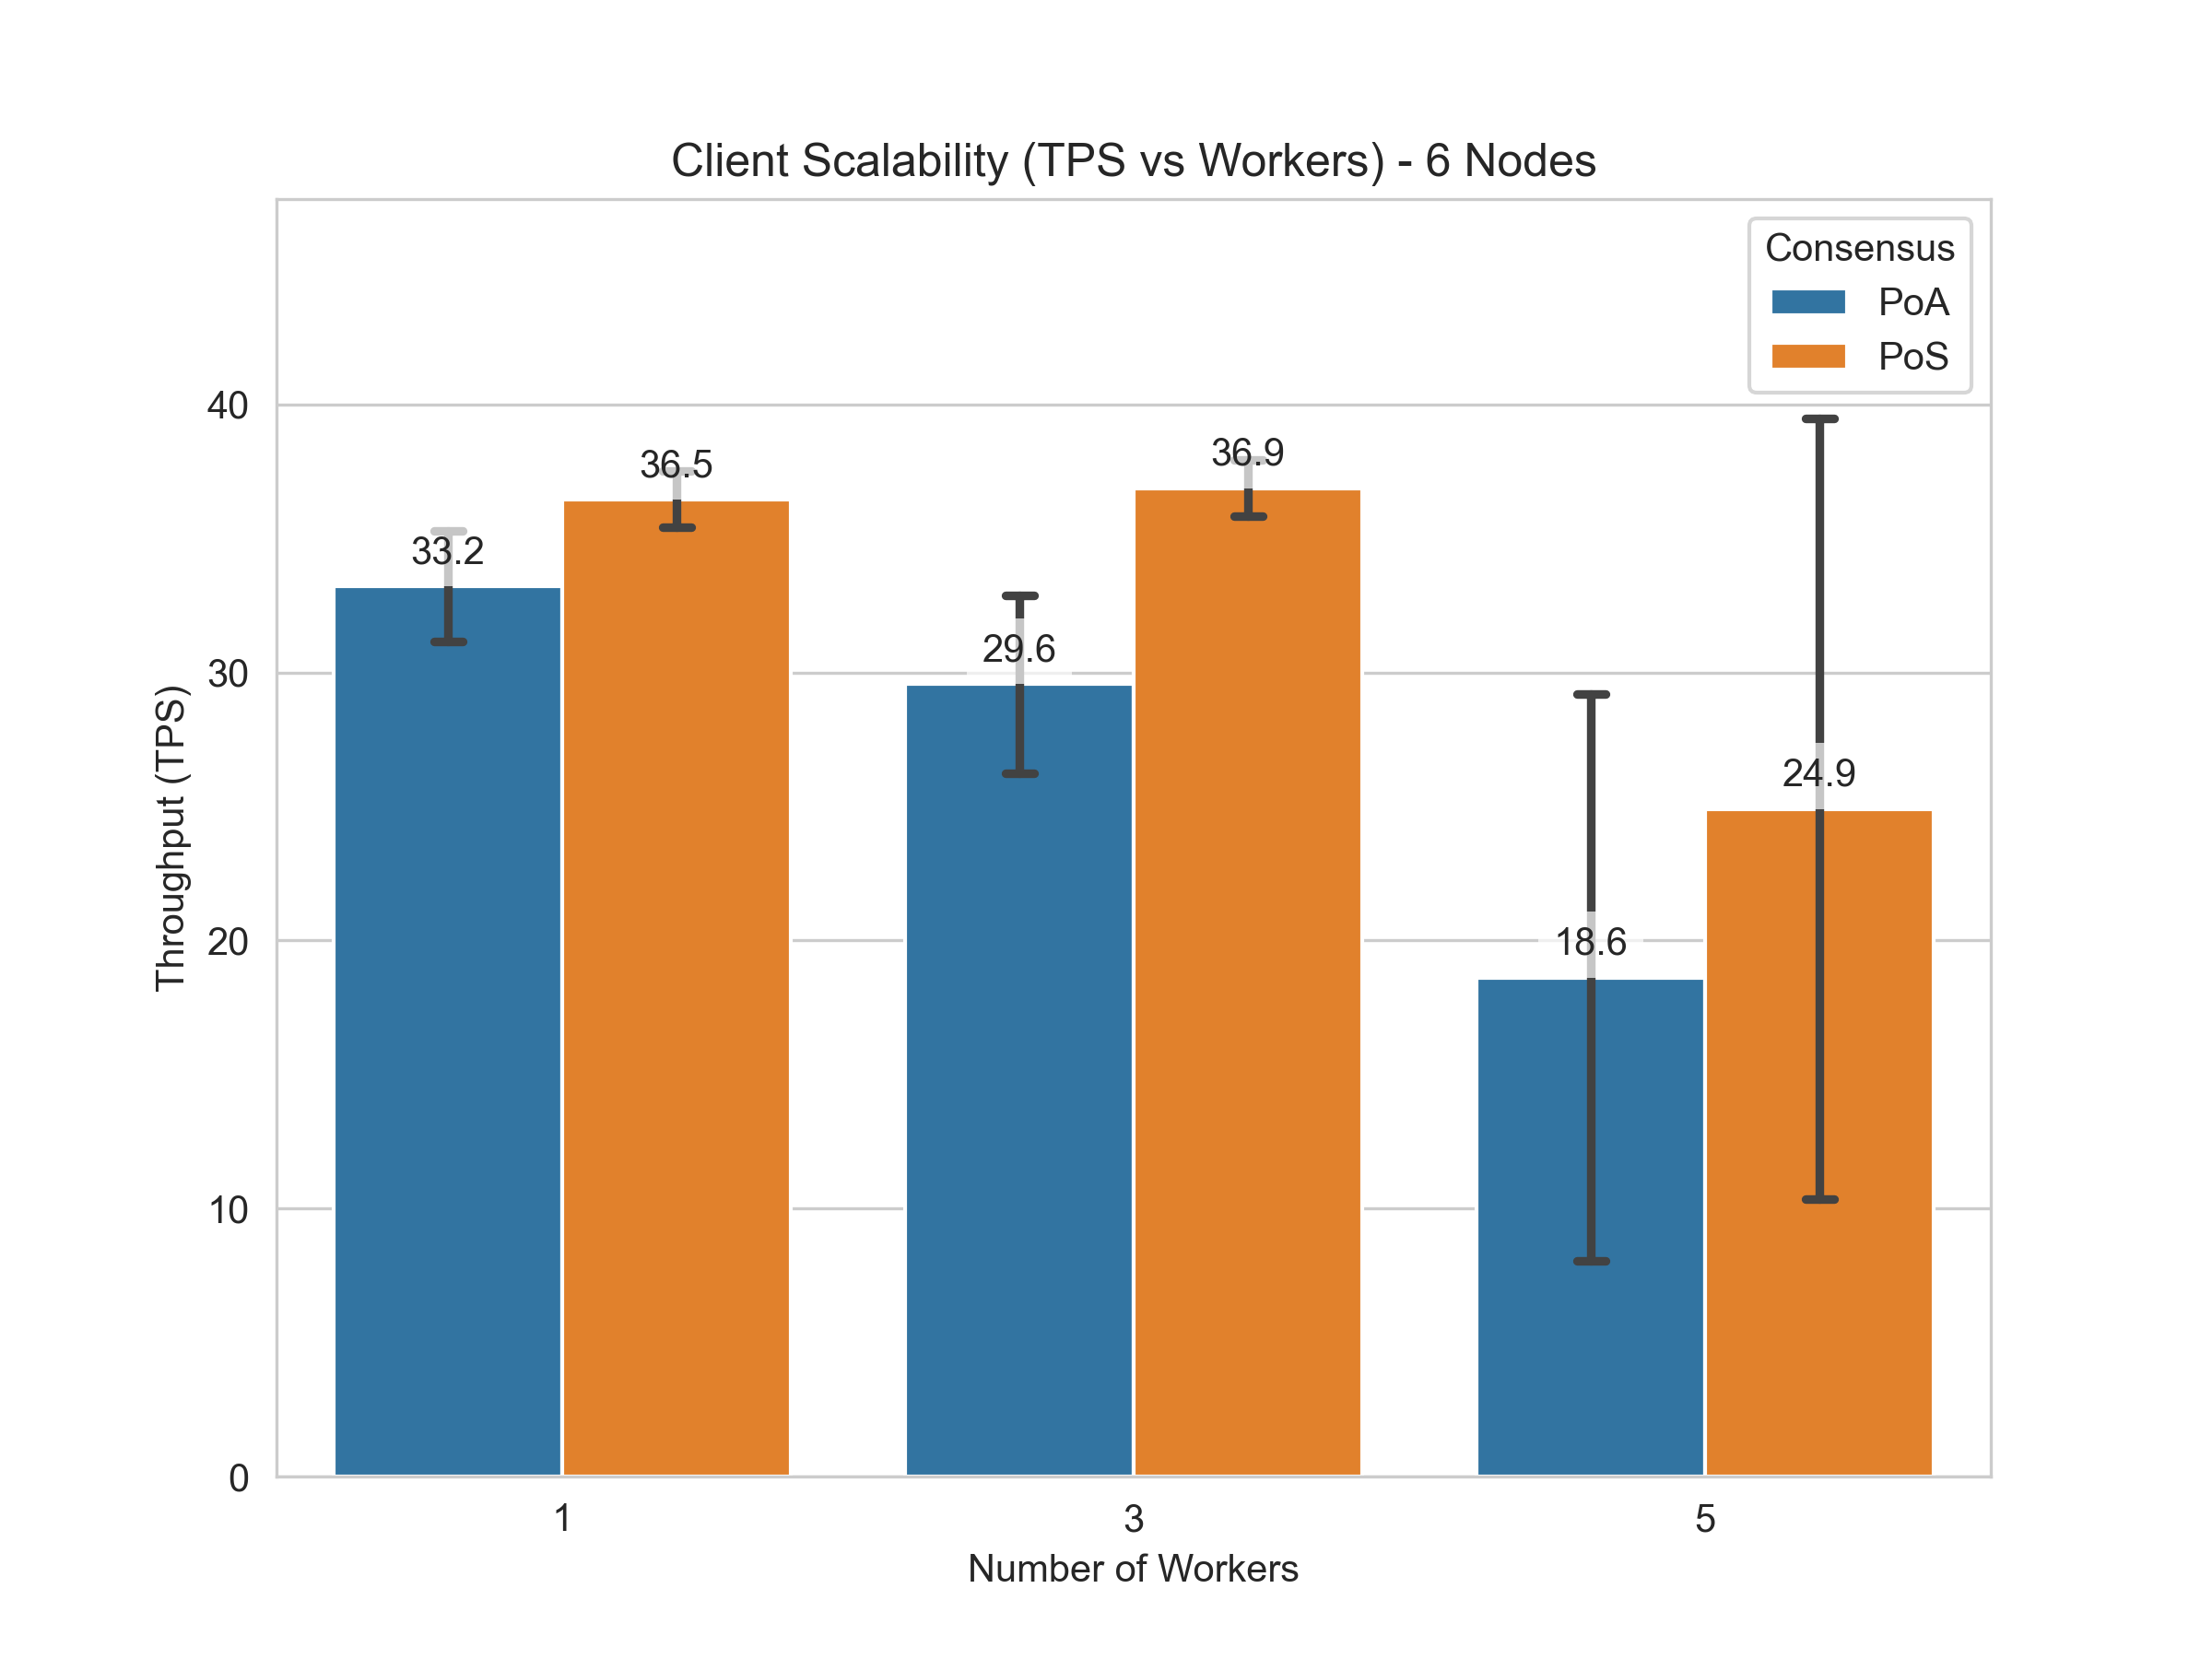
\includegraphics[width=0.9\textwidth]{images/scalability_client_tps_6_Nodes.png}
    \caption{Skalabilitas Klien pada Topologi 6 Node}
    \label{fig:scalability_client_6}
\end{figure}

\begin{figure}[htbp]
    \centering
    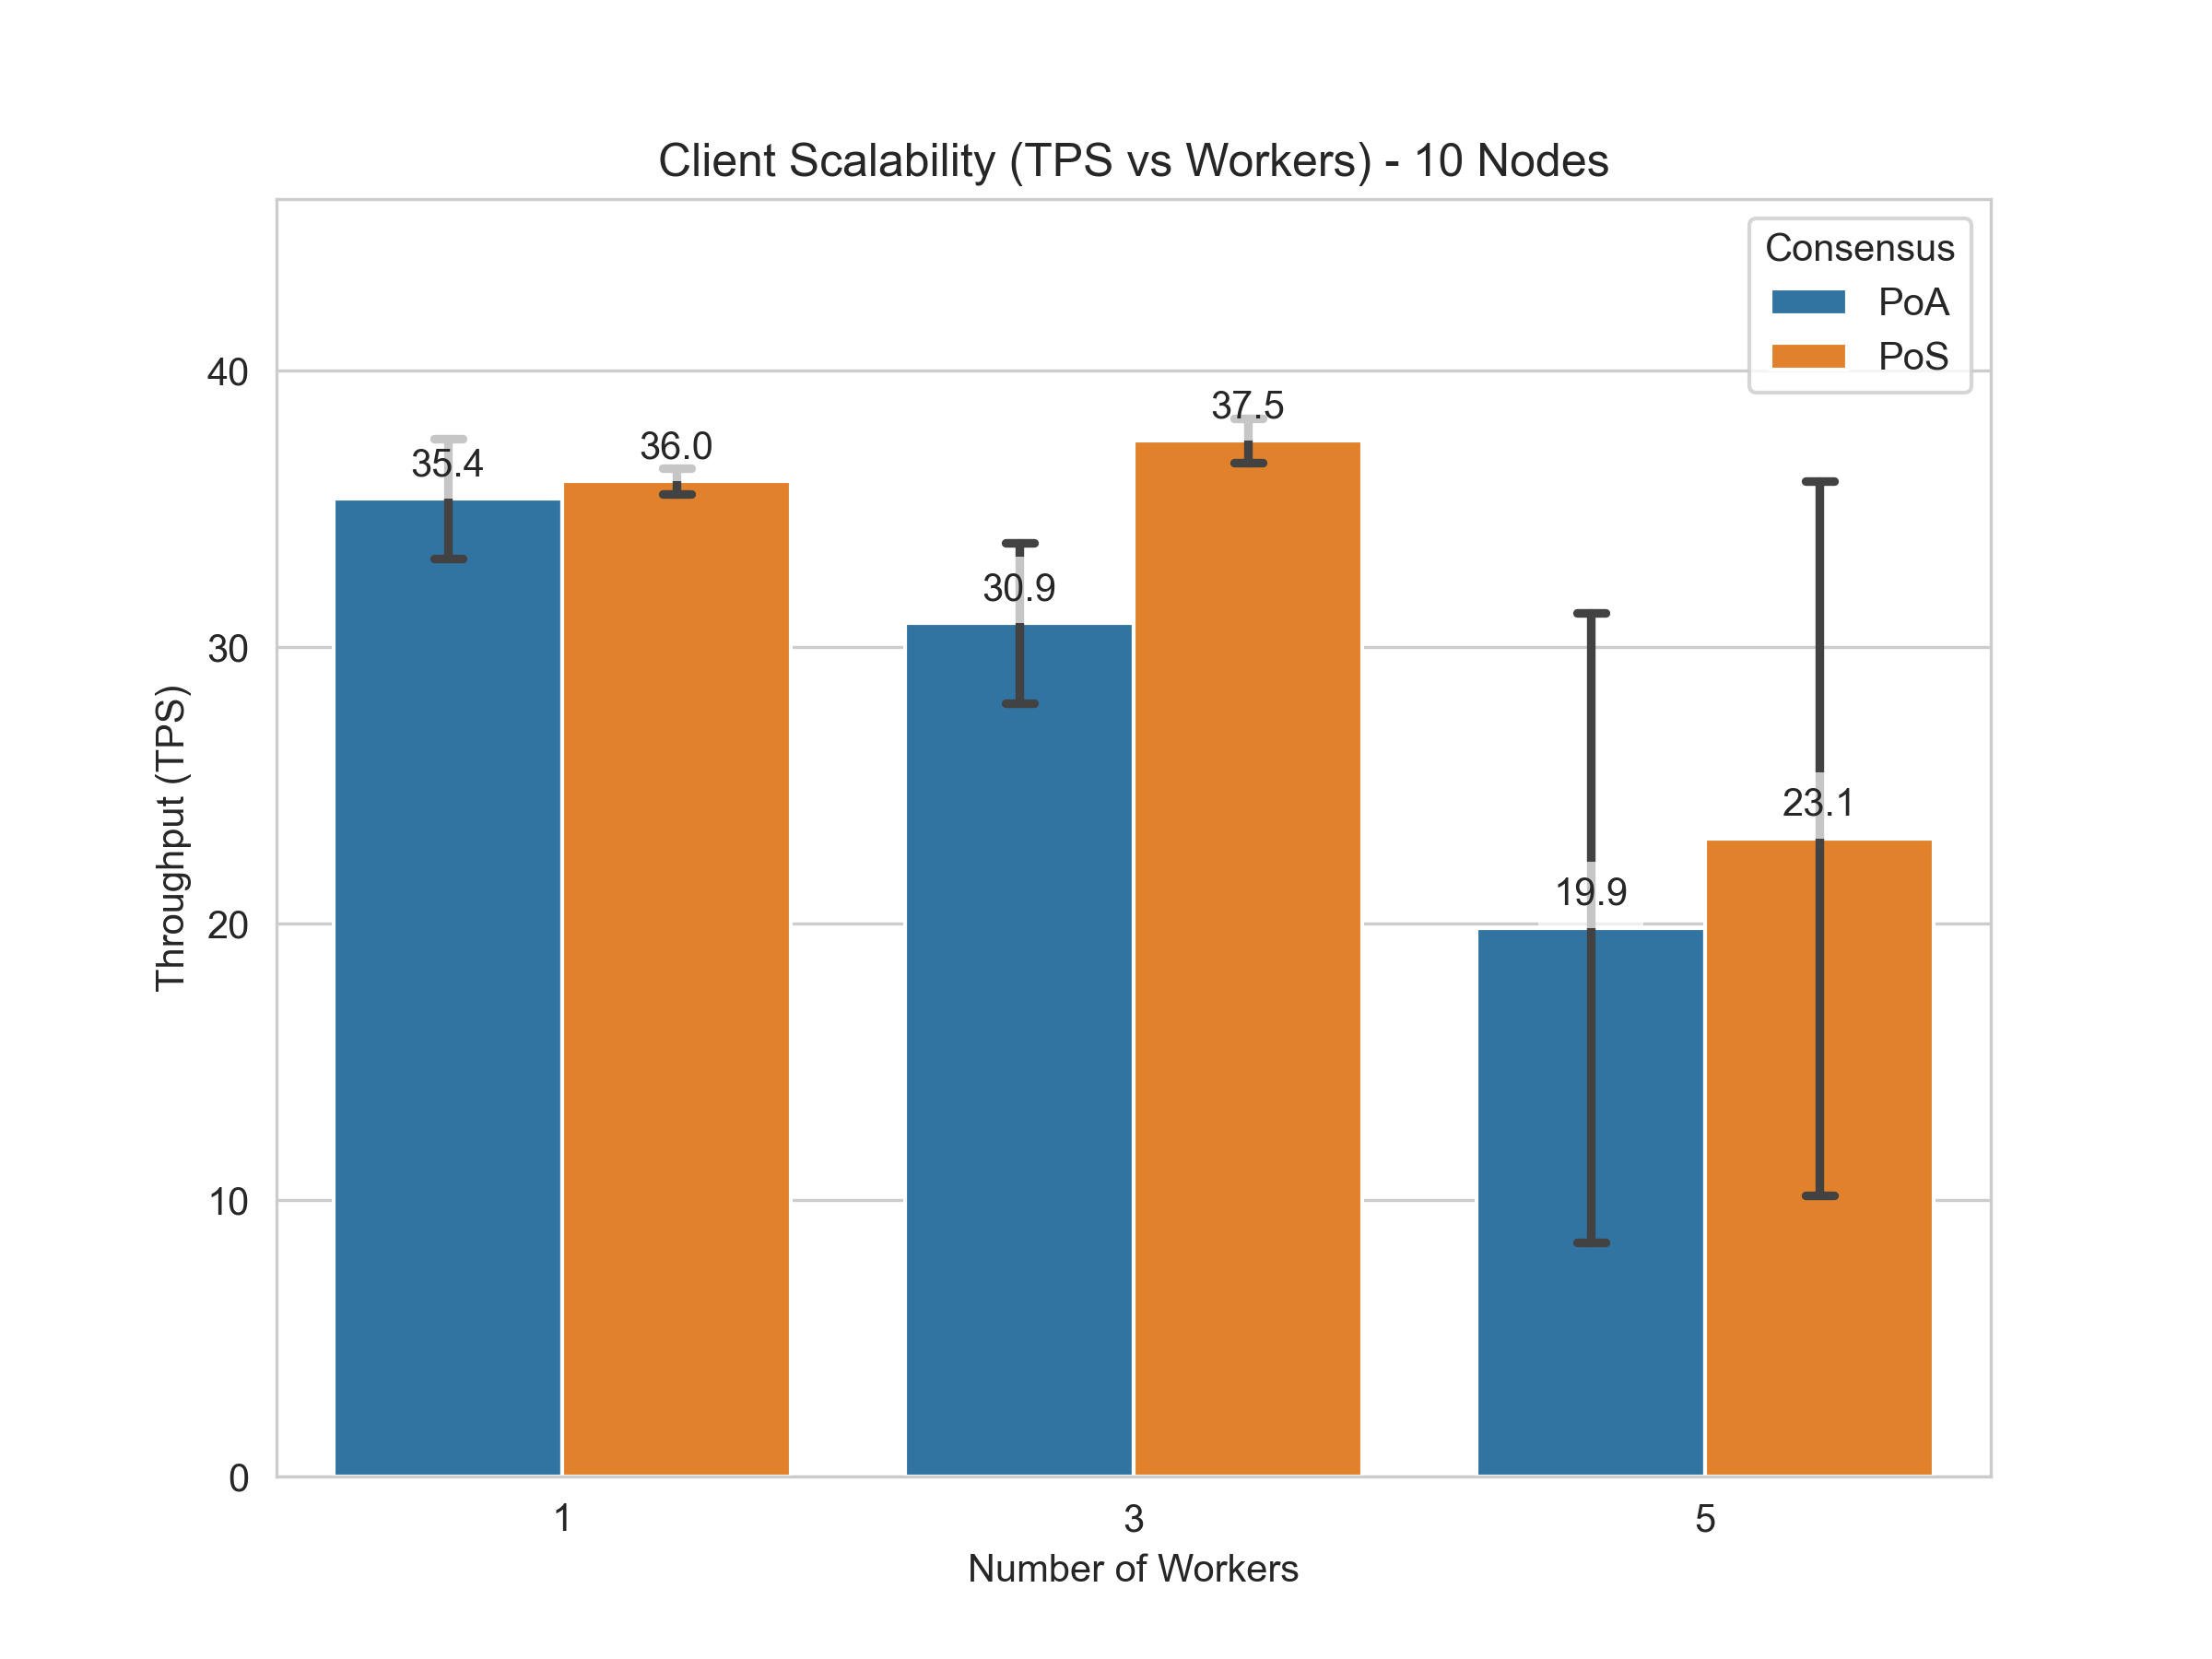
\includegraphics[width=0.9\textwidth]{images/scalability_client_tps_10_Nodes.png}
    \caption{Skalabilitas Klien pada Topologi 10 Node}
    \label{fig:scalability_client_10}
\end{figure}

\subsection{Stabilitas Jaringan (Soak Test)}

Uji durabilitas (\textit{Soak Test}) selama 15 menit dilakukan untuk memverifikasi kestabilan jaringan. Hasilnya dapat dilihat pada grafik \textit{Time Series} TPS (Gambar \ref{fig:stability_timeseries_tps_4}, \ref{fig:stability_timeseries_tps_6}, \ref{fig:stability_timeseries_tps_10}).

Garis yang mendatar (flat) pada grafik time-series TPS menunjukkan stabilitas yang sangat baik. Hal serupa juga terlihat pada stabilitas latensi (Gambar \ref{fig:stability_timeseries_latency_4}, \ref{fig:stability_timeseries_latency_6}, \ref{fig:stability_timeseries_latency_10}), di mana waktu respons tetap konsisten sepanjang pengujian tanpa adanya lonjakan (*spike*) yang tidak wajar. Baik PoA maupun PoS mampu mempertahankan performa yang konstan selama durasi pengujian.
Namun, jika dilihat dari Gambar \ref{fig:stability_cv} yang membandingkan \textit{Coefficient of Variation} (CV), PoA memiliki nilai CV yang sedikit lebih rendah di beberapa skenario, mengindikasikan variabilitas performa yang lebih kecil (lebih deterministik) dibandingkan PoS yang memiliki variasi probabilistik antar-blok.

\begin{figure}[htbp]
    \centering
    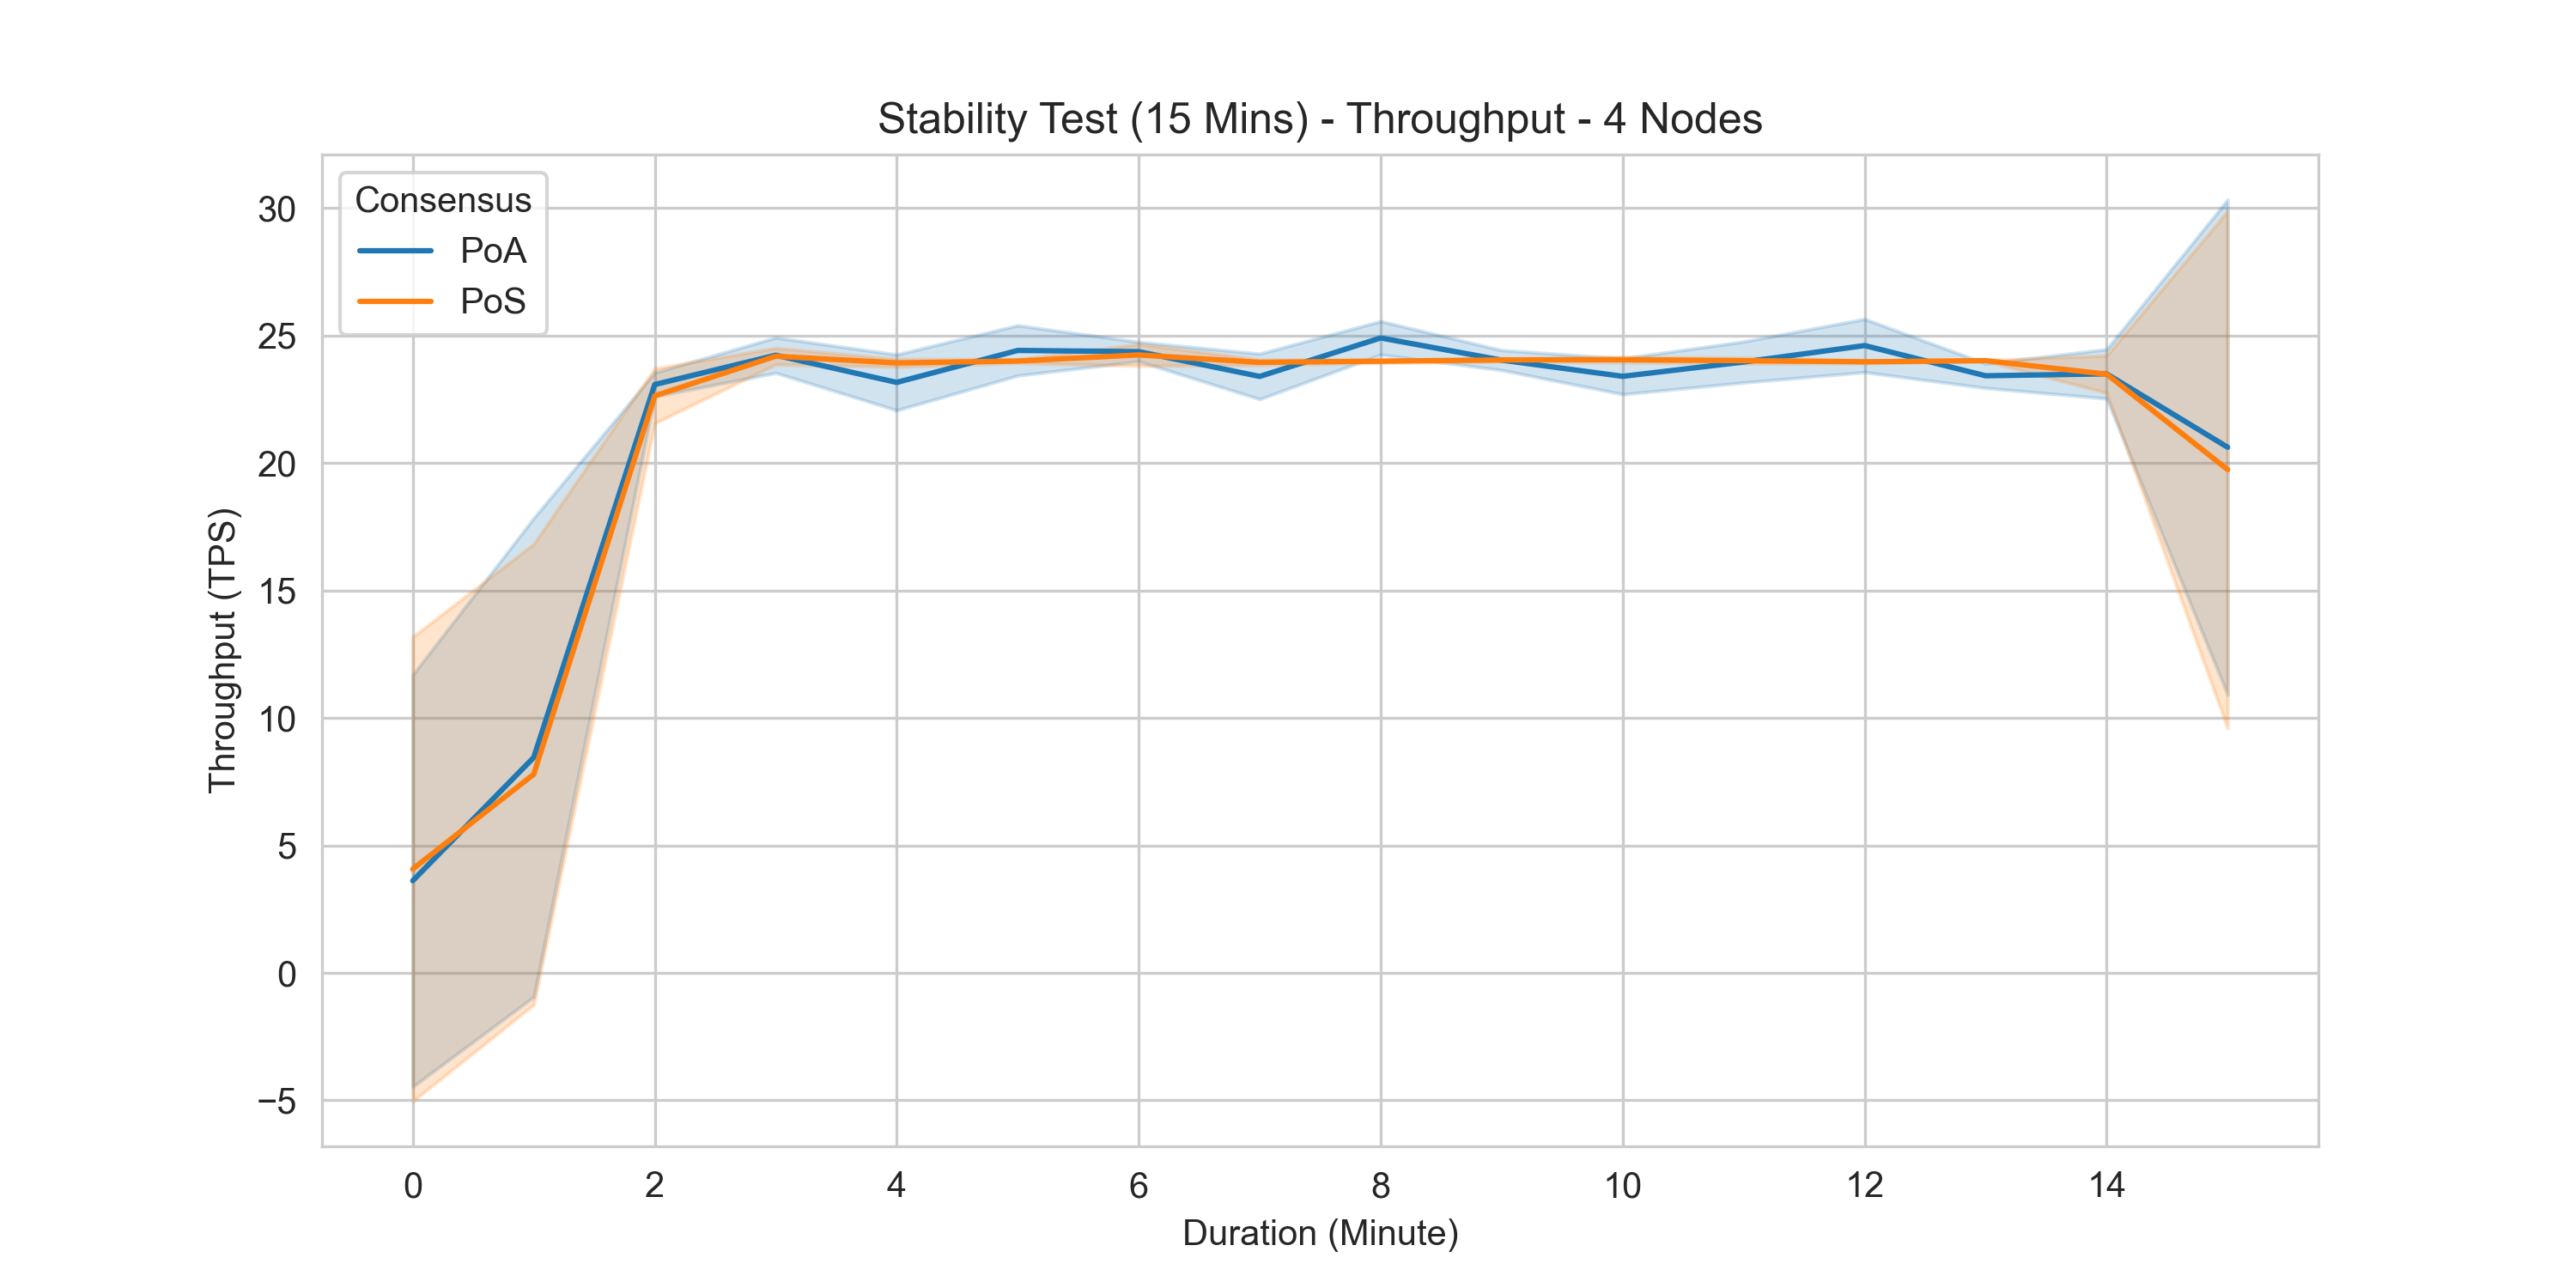
\includegraphics[width=0.9\textwidth]{images/stability_timeseries_tps_4_Nodes.png}
    \caption{Time Series TPS pada Uji Stabilitas (4 Node)}
    \label{fig:stability_timeseries_tps_4}
\end{figure}

\begin{figure}[htbp]
    \centering
    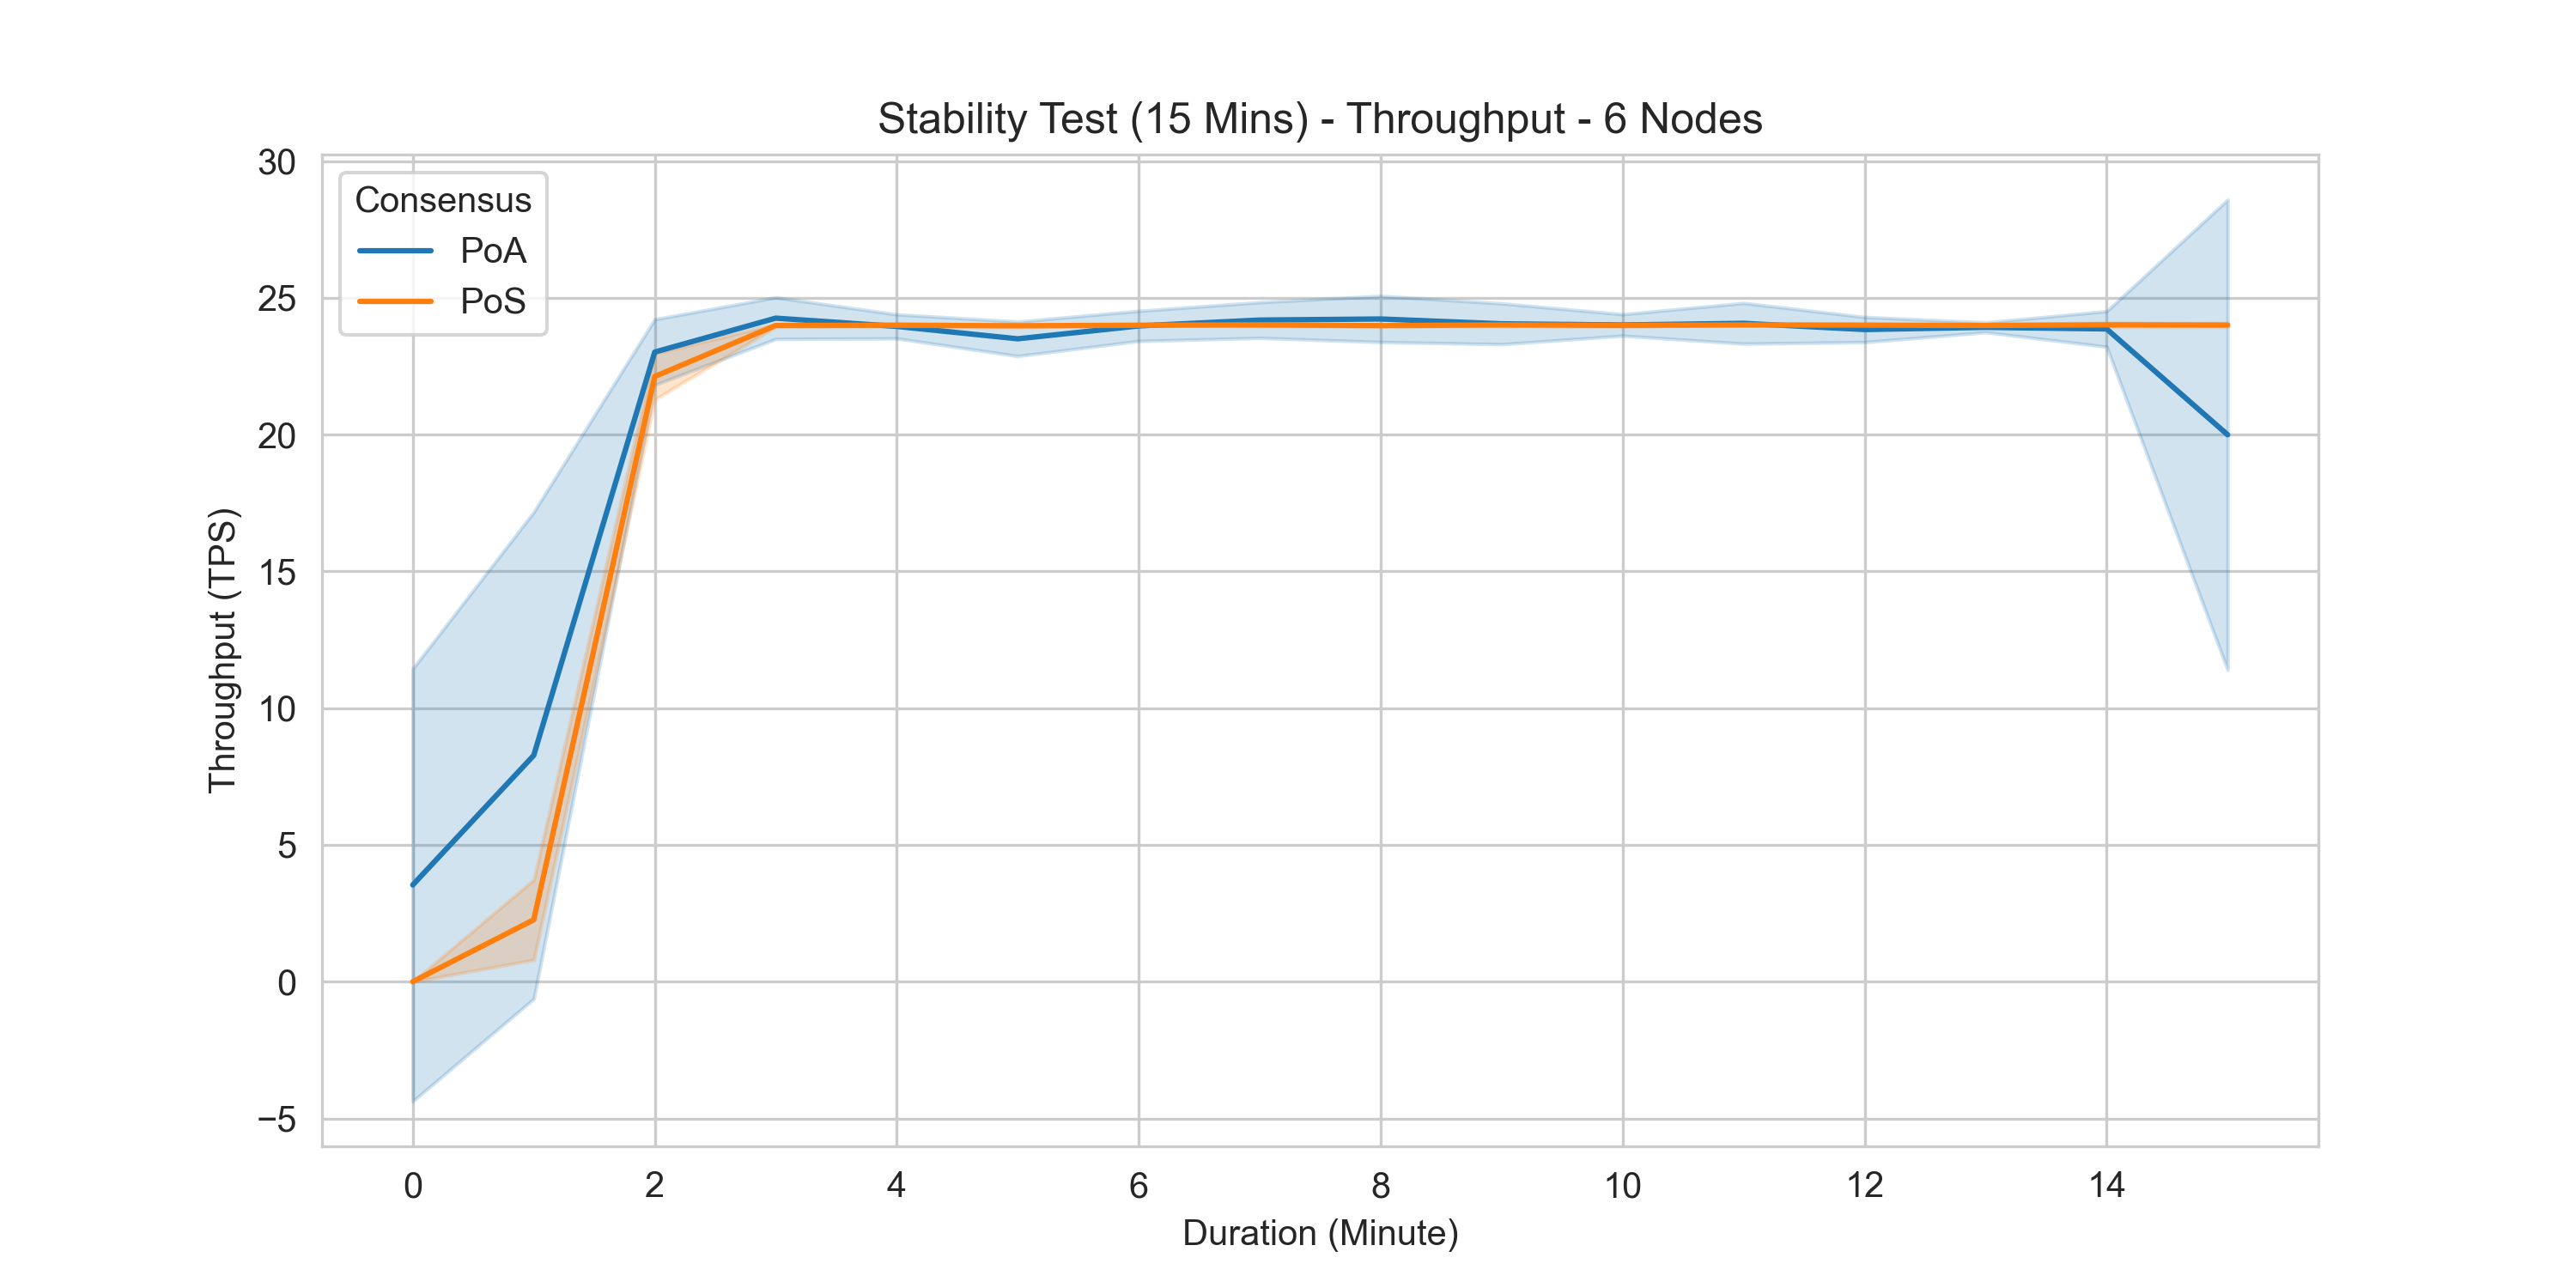
\includegraphics[width=0.9\textwidth]{images/stability_timeseries_tps_6_Nodes.png}
    \caption{Time Series TPS pada Uji Stabilitas (6 Node)}
    \label{fig:stability_timeseries_tps_6}
\end{figure}

\begin{figure}[htbp]
    \centering
    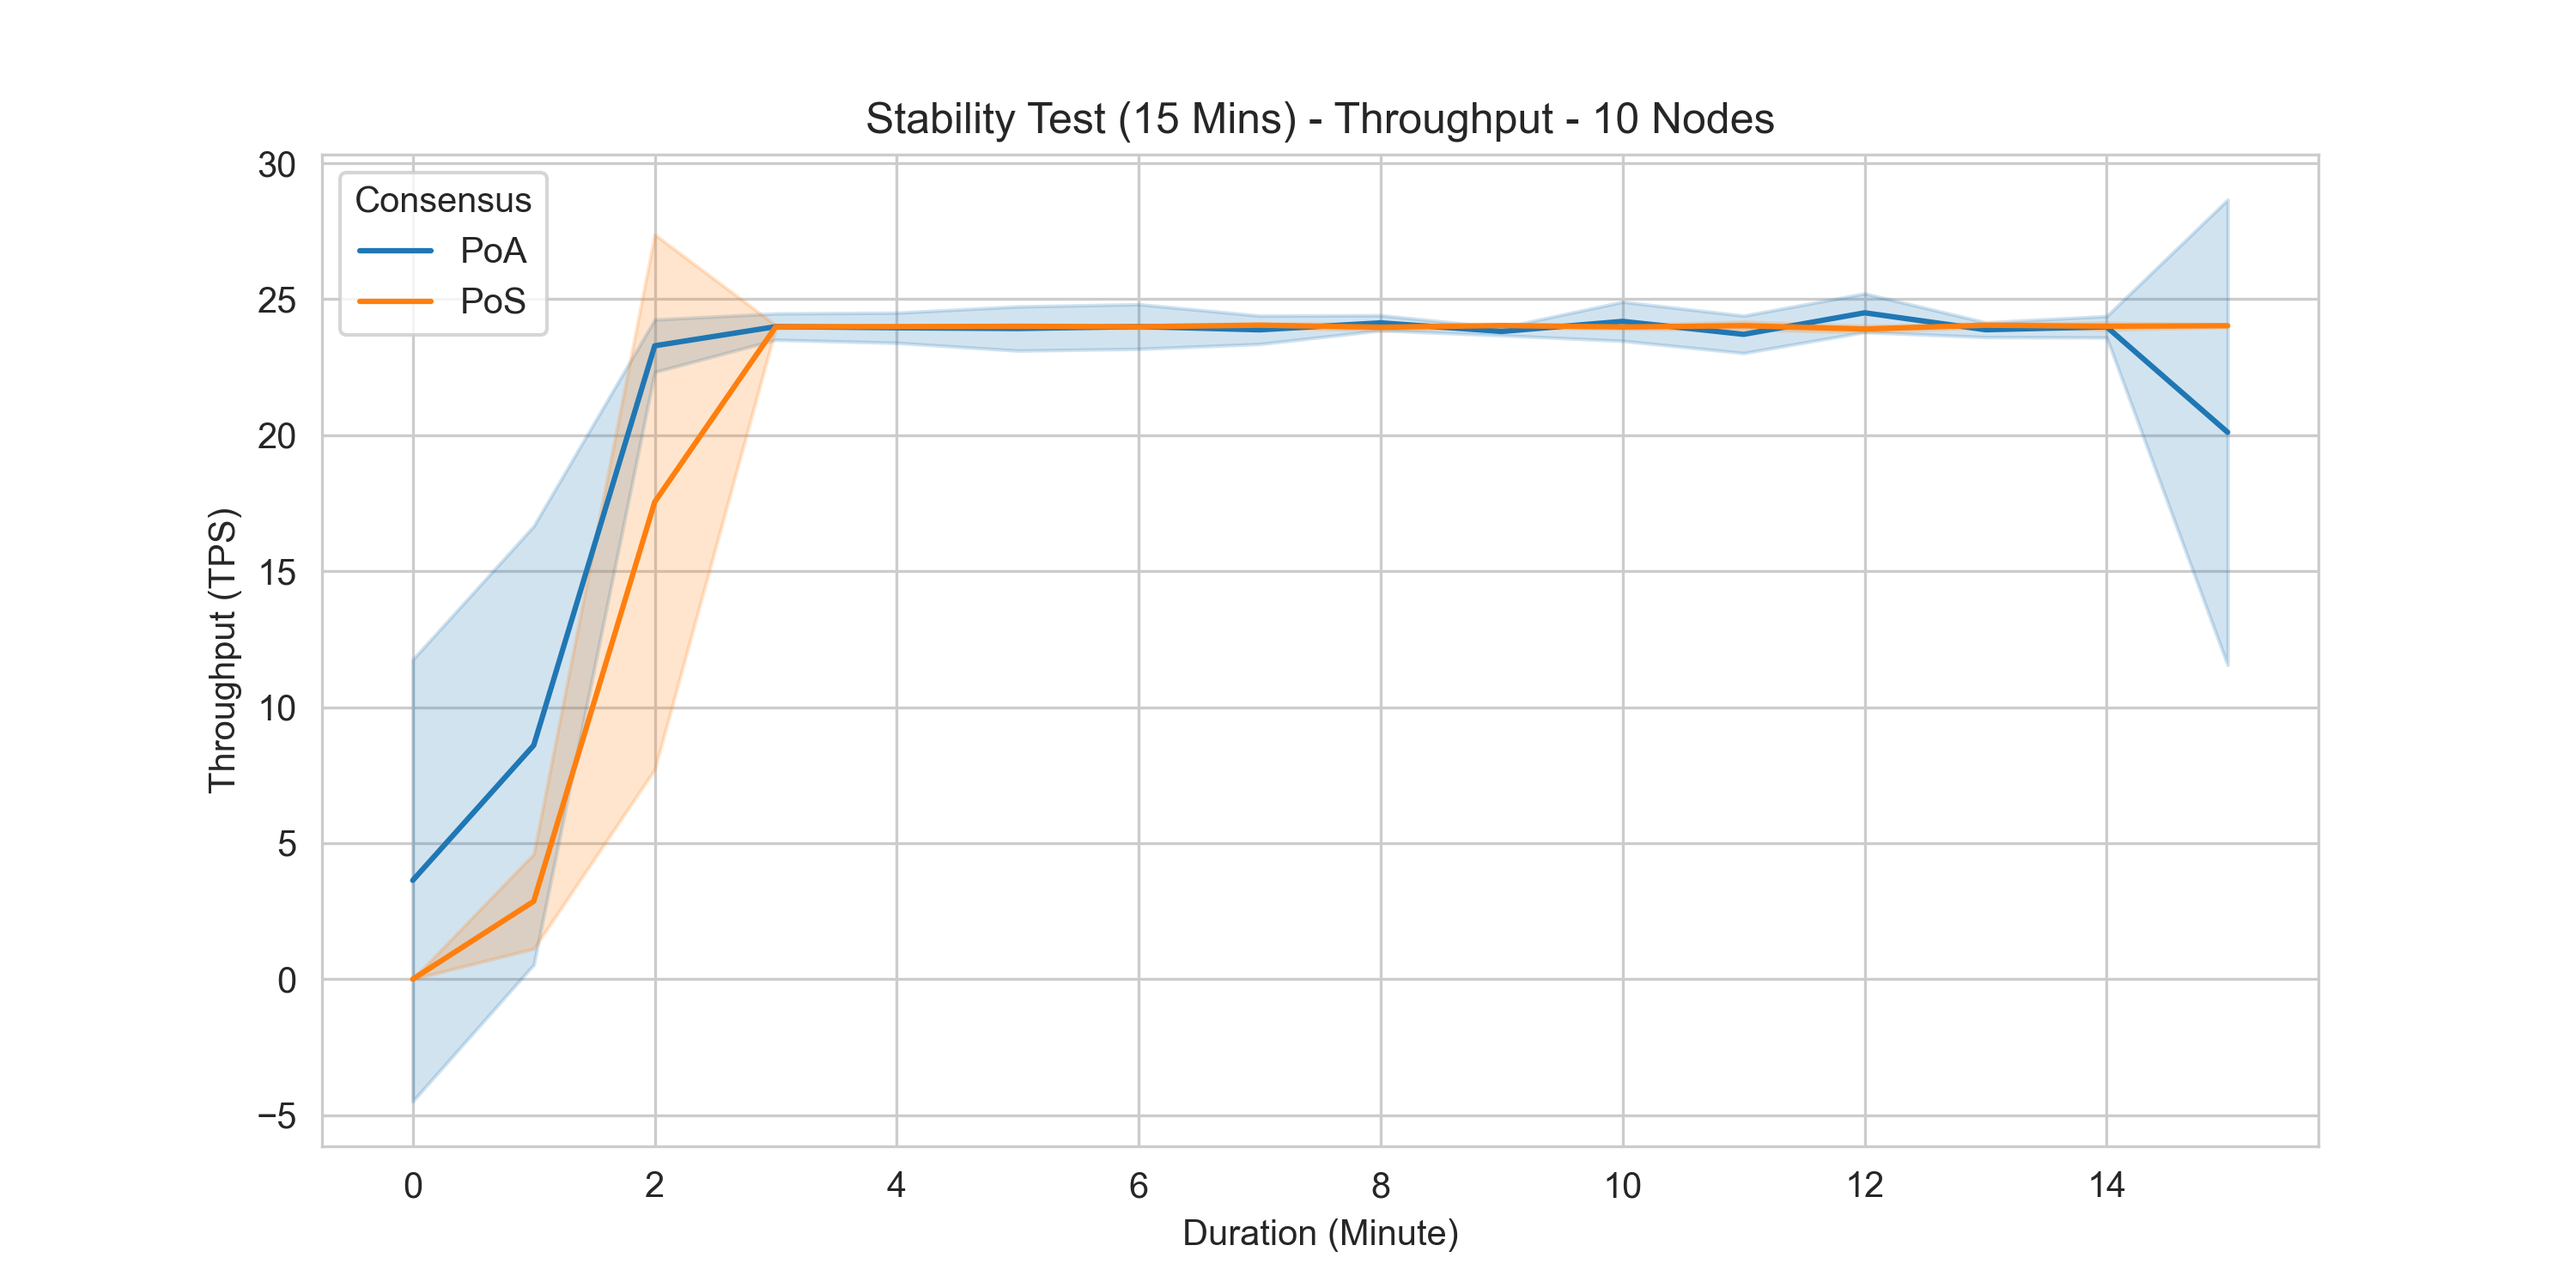
\includegraphics[width=0.9\textwidth]{images/stability_timeseries_tps_10_Nodes.png}
    \caption{Time Series TPS pada Uji Stabilitas (10 Node)}
    \label{fig:stability_timeseries_tps_10}
\end{figure}

\begin{figure}[htbp]
    \centering
    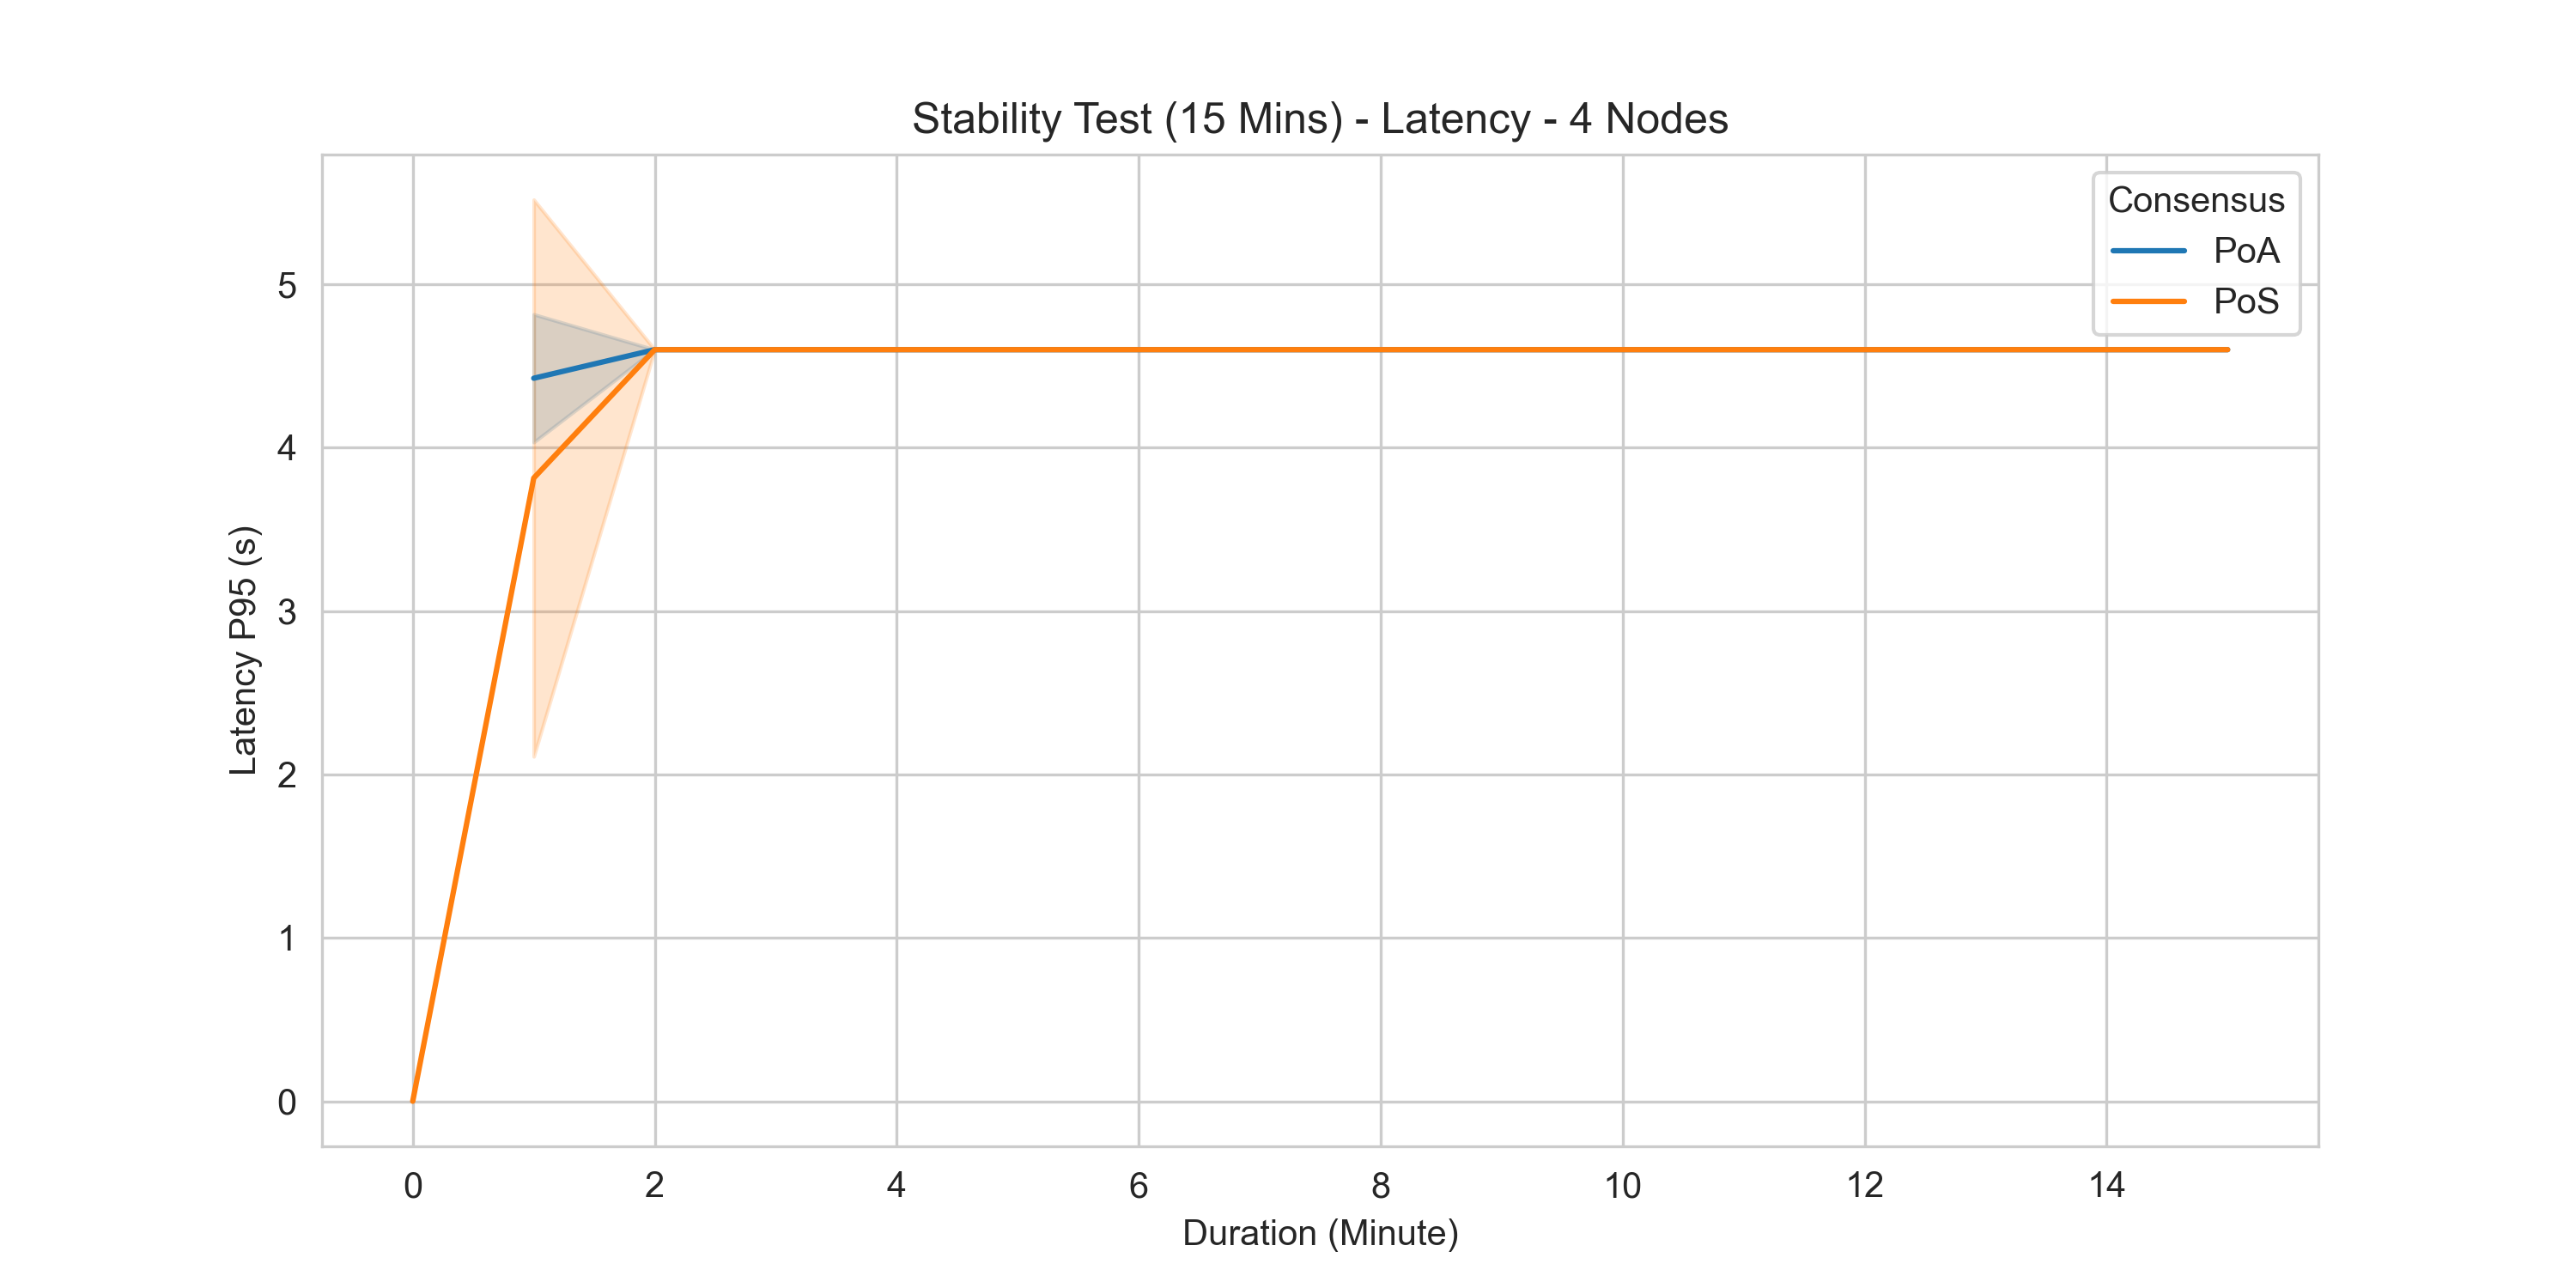
\includegraphics[width=0.9\textwidth]{images/stability_timeseries_latency_4_Nodes.png}
    \caption{Time Series Latency pada Uji Stabilitas (4 Node)}
    \label{fig:stability_timeseries_latency_4}
\end{figure}

\begin{figure}[htbp]
    \centering
    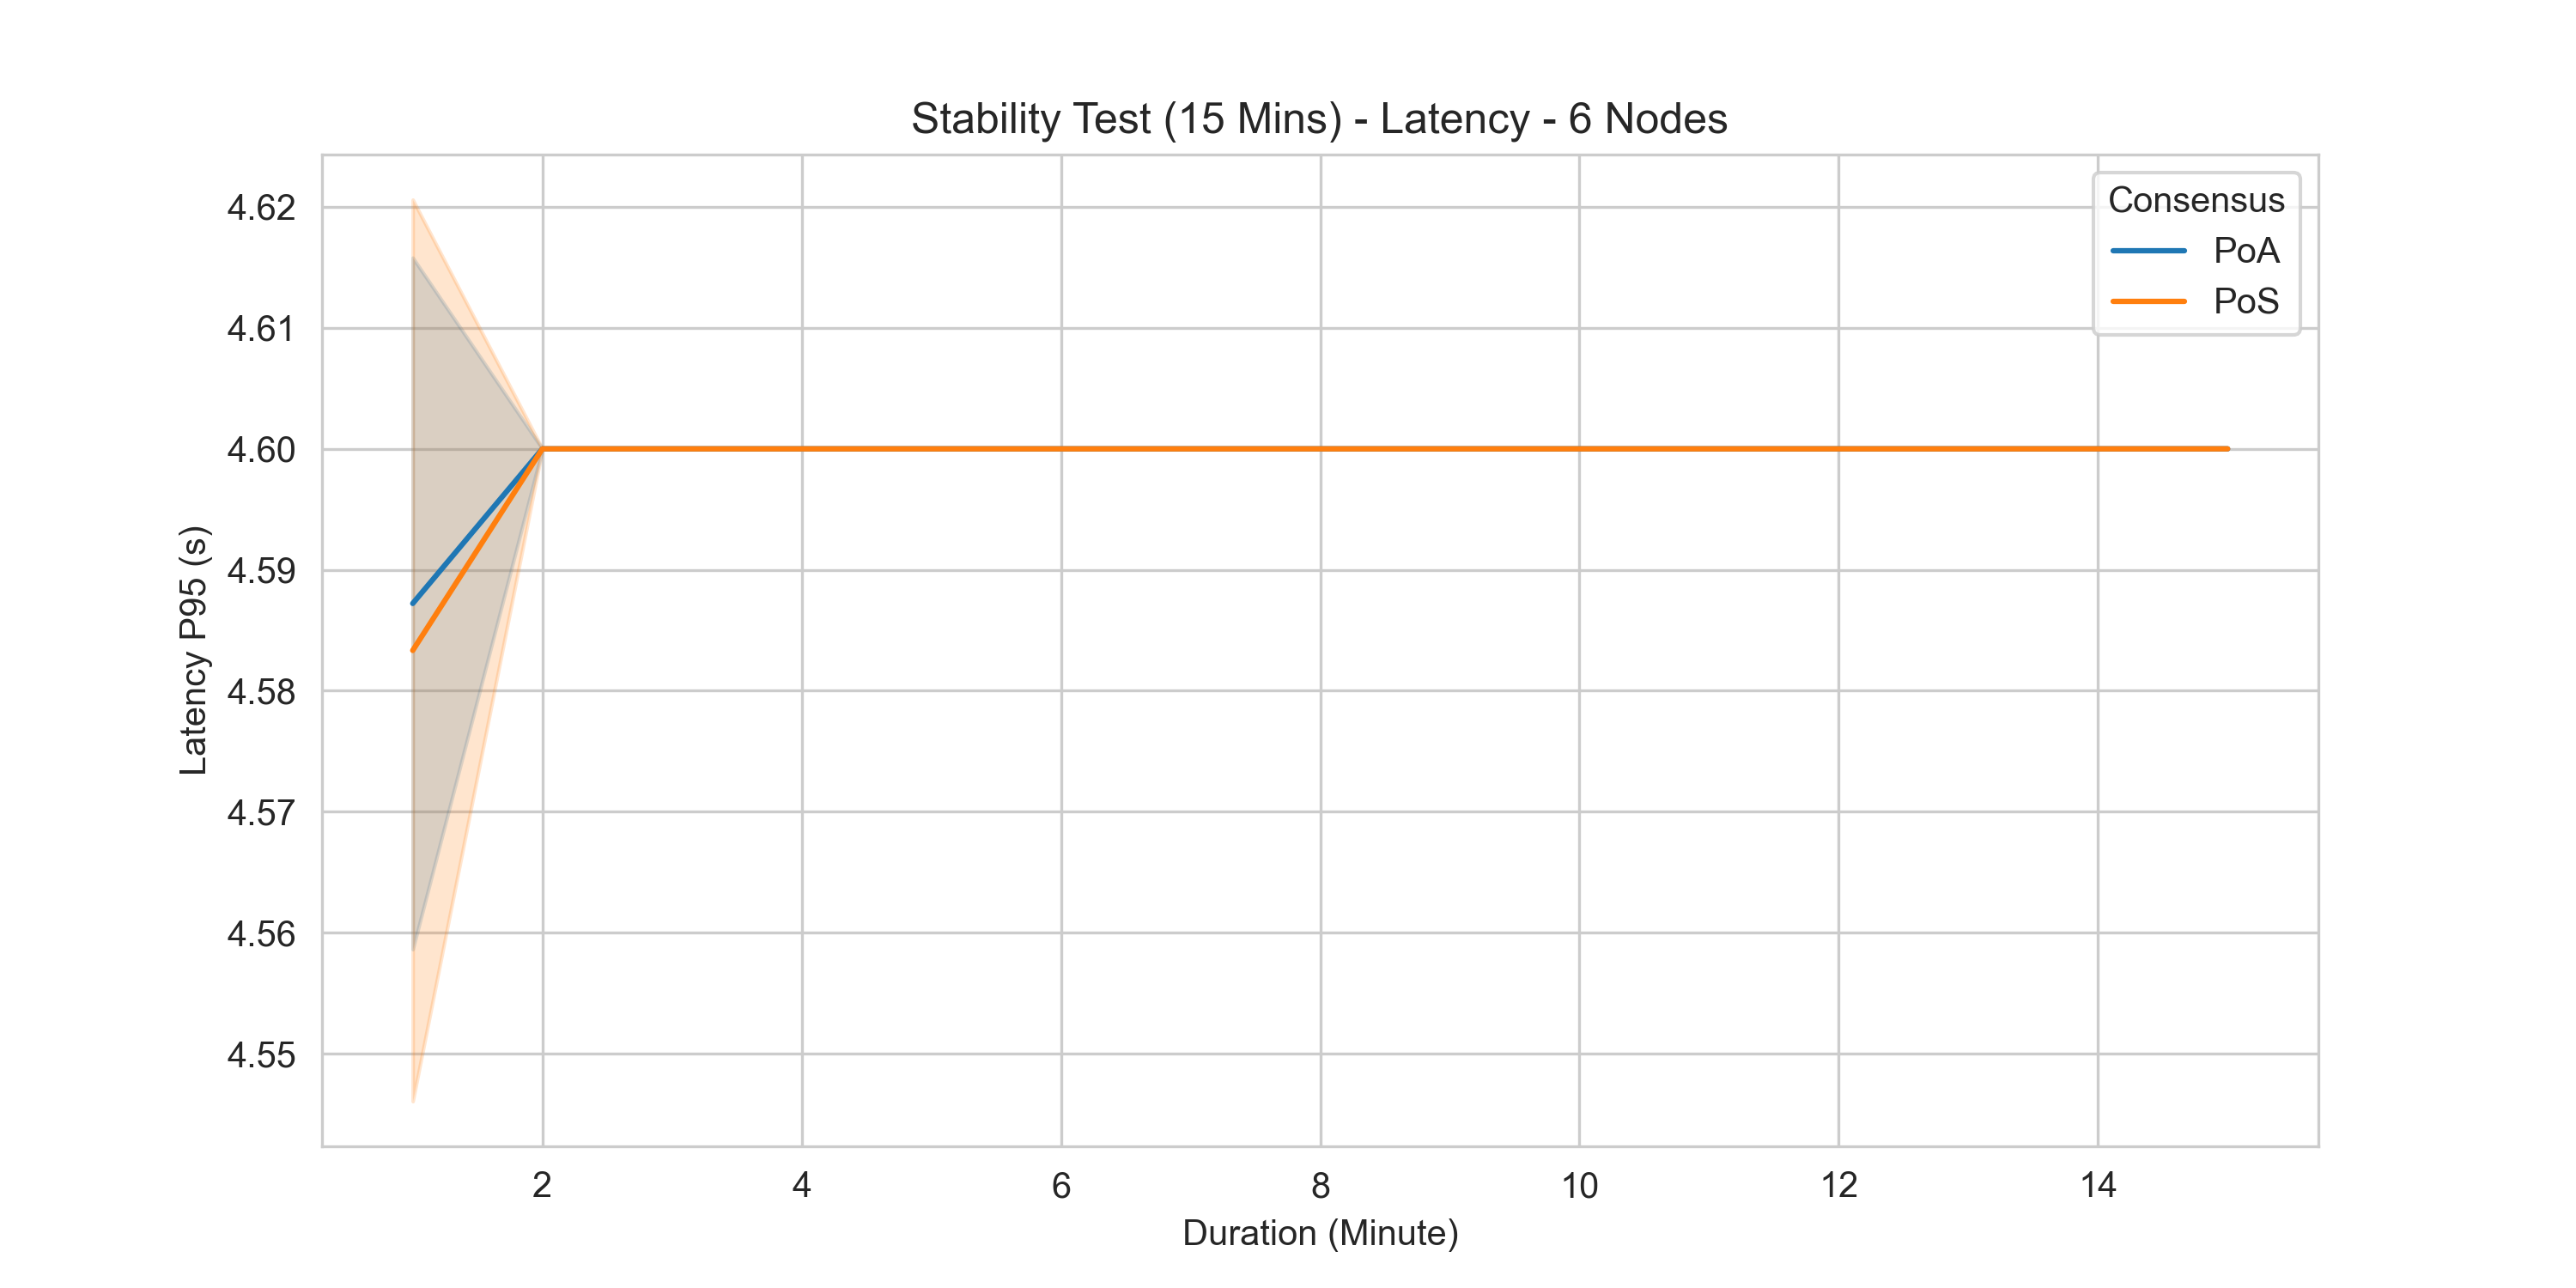
\includegraphics[width=0.9\textwidth]{images/stability_timeseries_latency_6_Nodes.png}
    \caption{Time Series Latency pada Uji Stabilitas (6 Node)}
    \label{fig:stability_timeseries_latency_6}
\end{figure}

\begin{figure}[htbp]
    \centering
    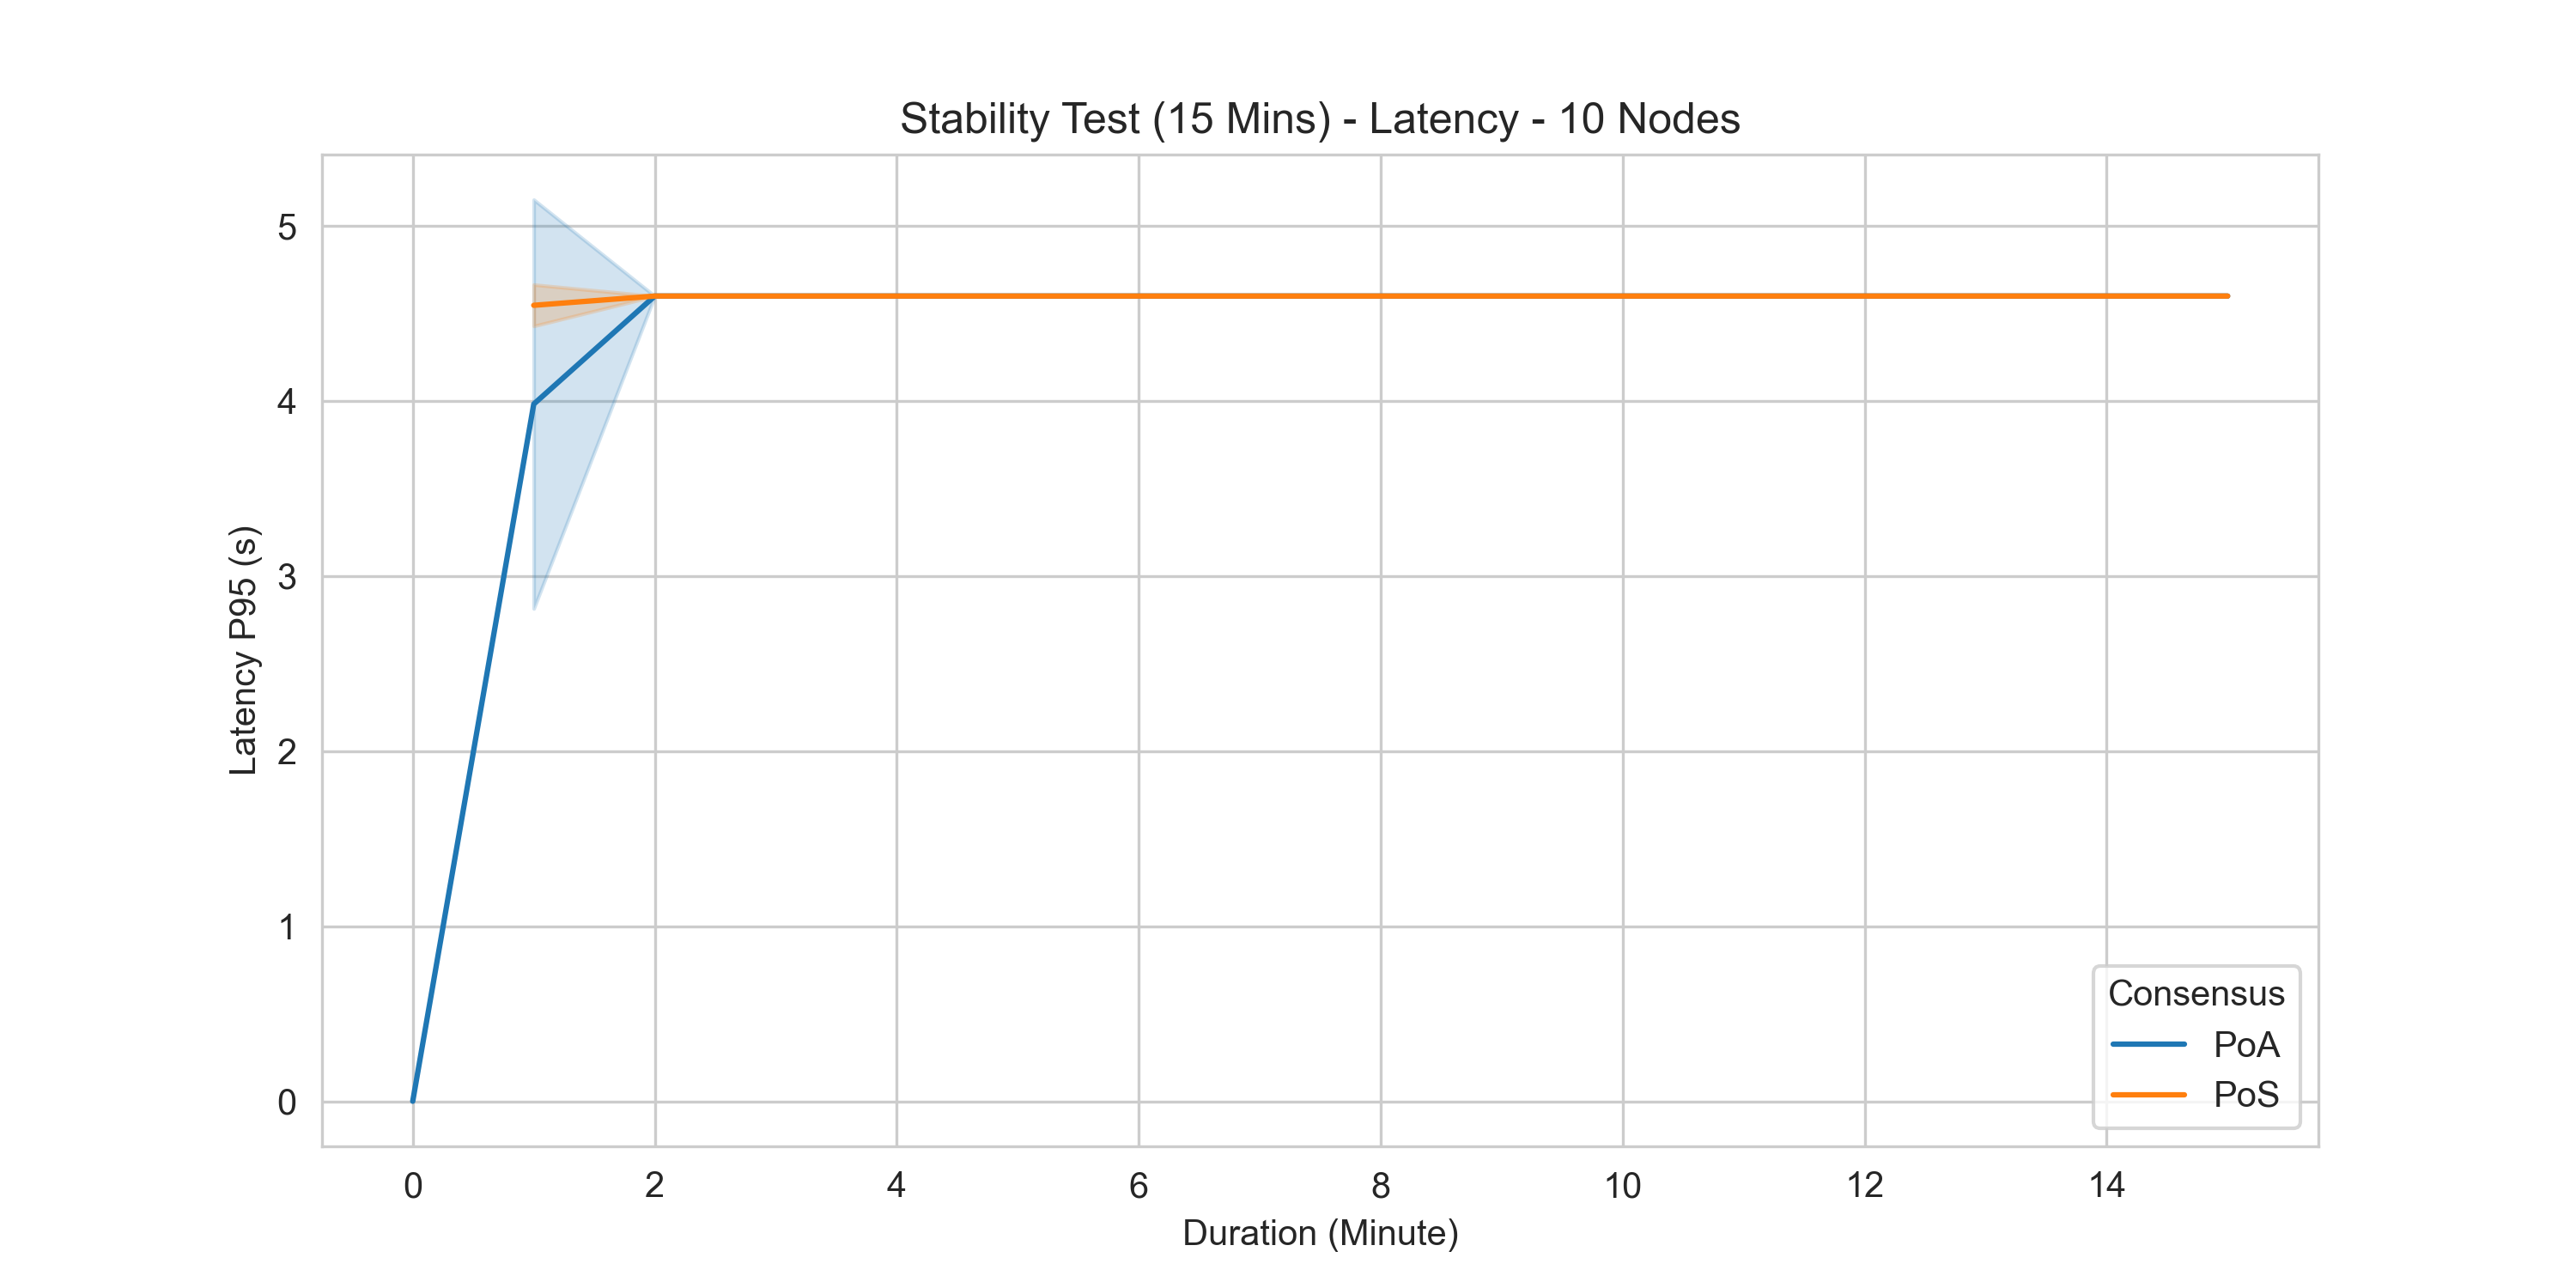
\includegraphics[width=0.9\textwidth]{images/stability_timeseries_latency_10_Nodes.png}
    \caption{Time Series Latency pada Uji Stabilitas (10 Node)}
    \label{fig:stability_timeseries_latency_10}
\end{figure}

\begin{figure}[htbp]
    \centering
    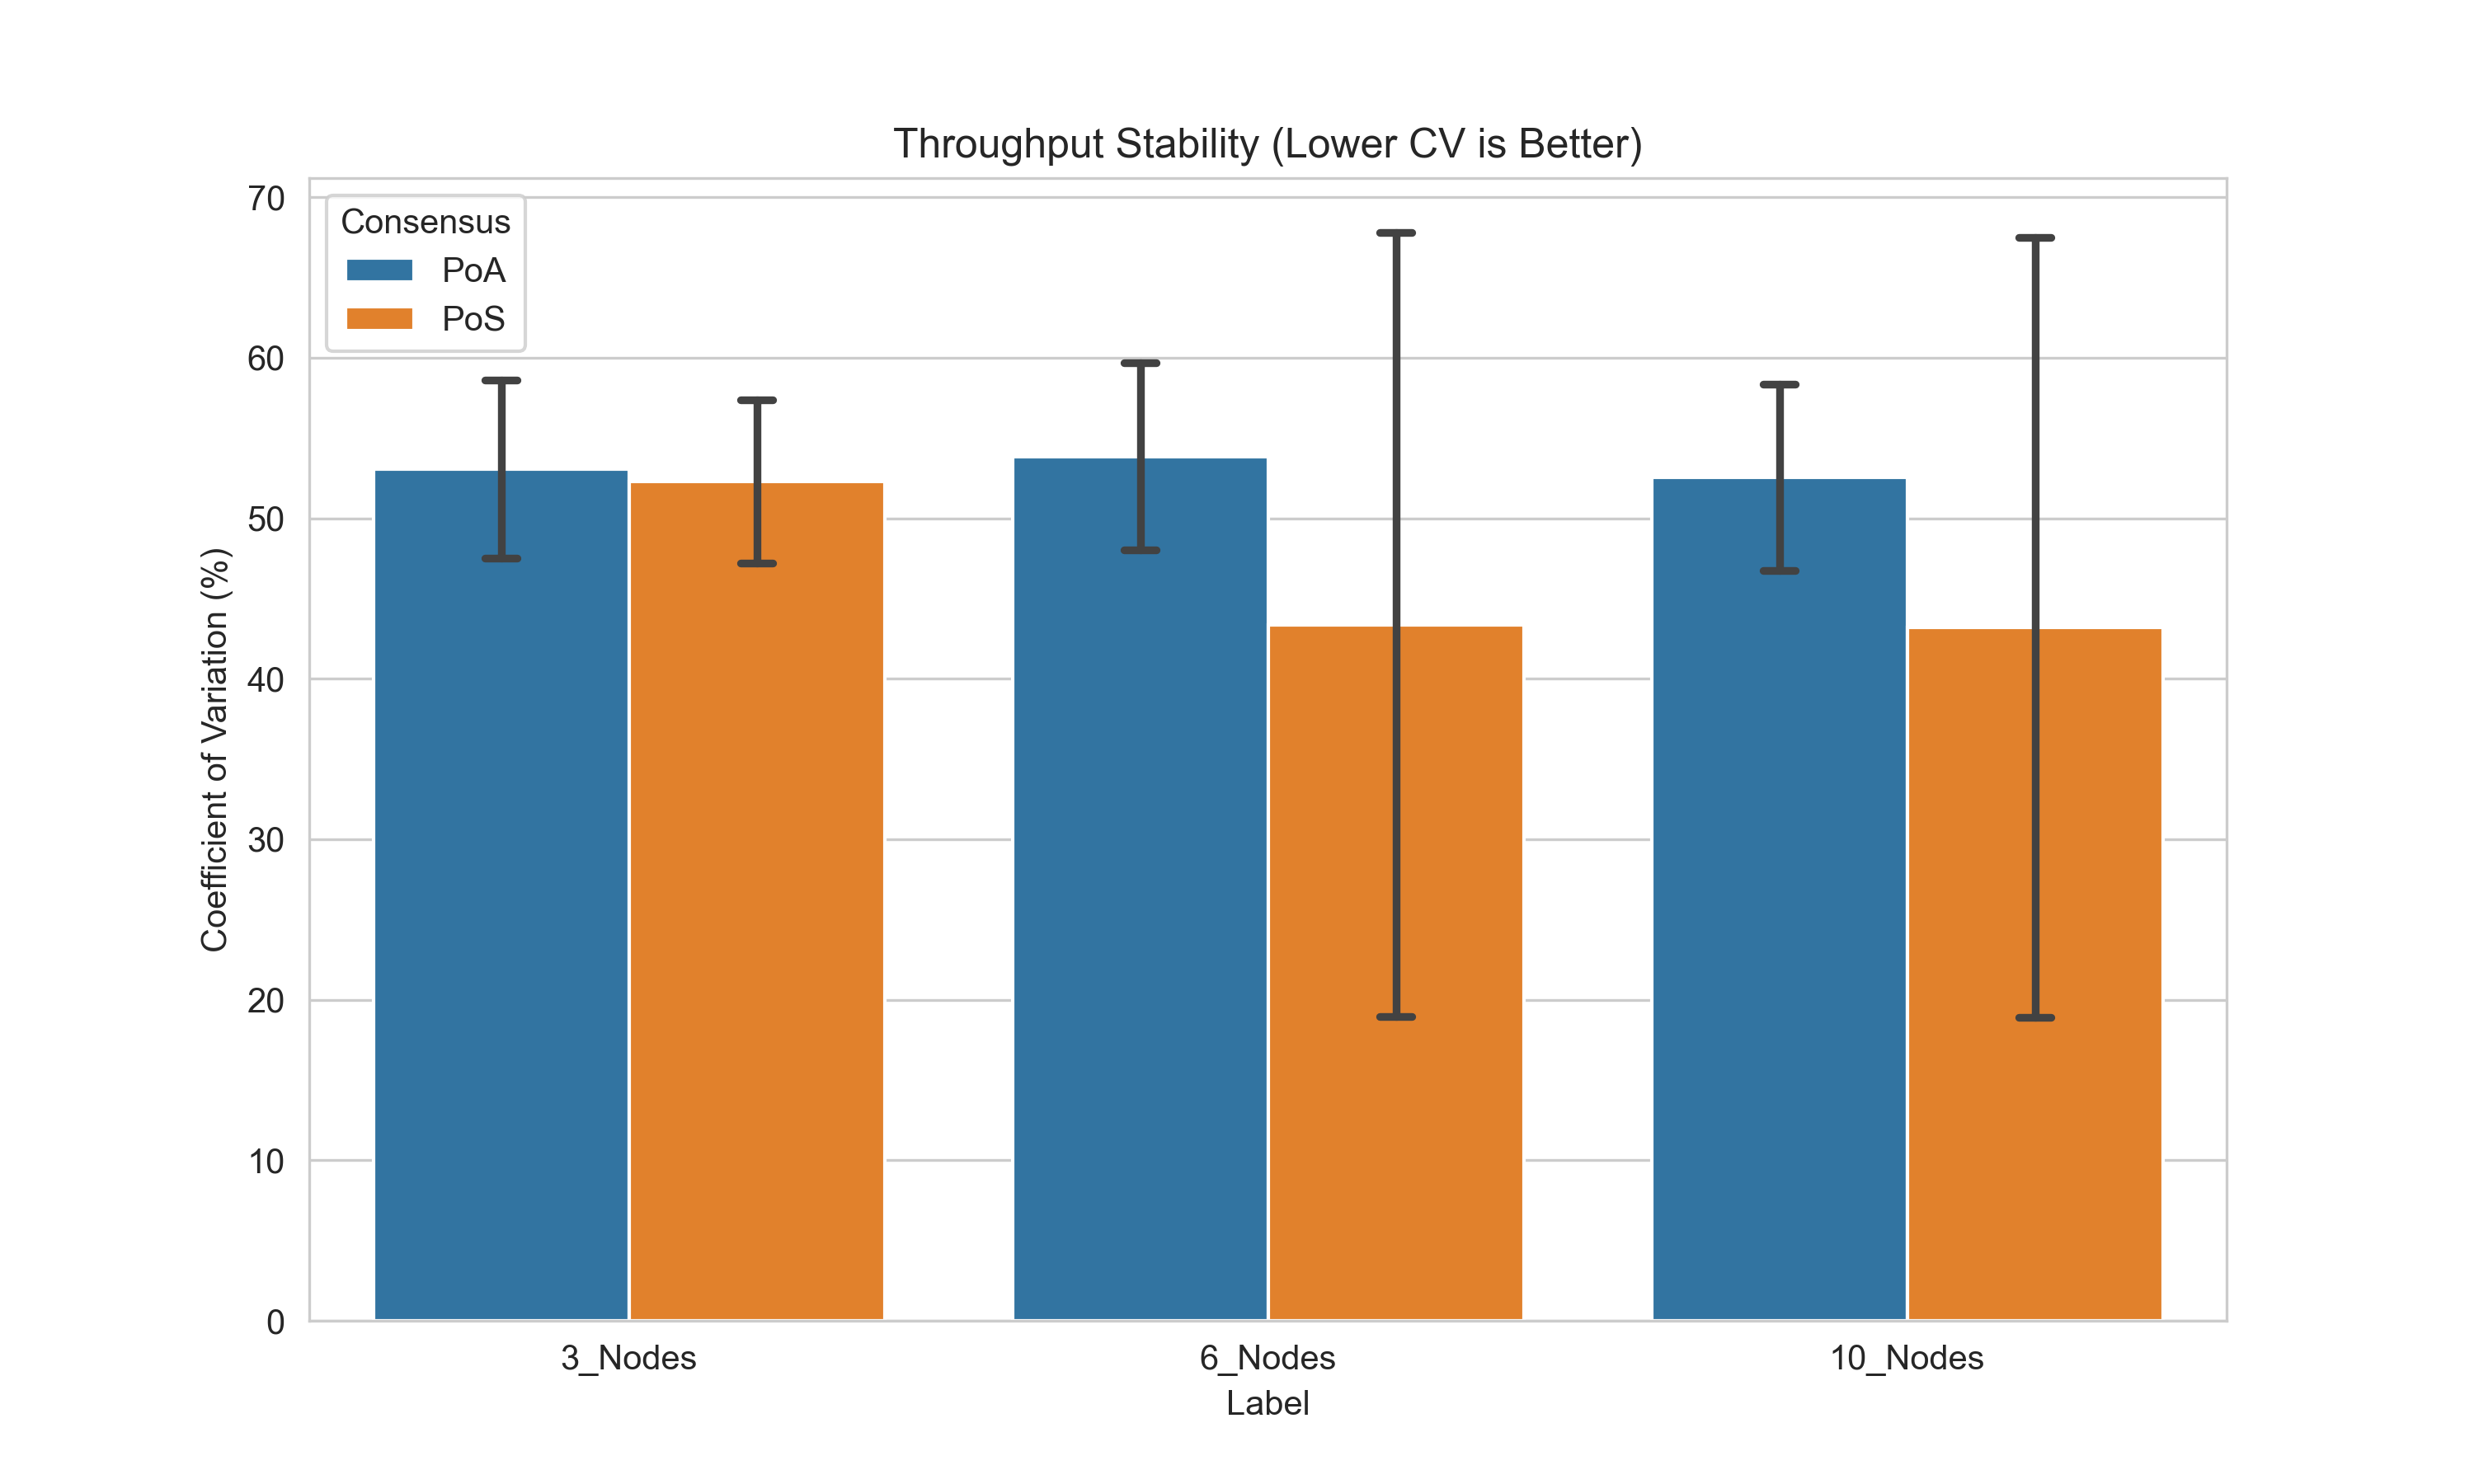
\includegraphics[width=0.9\textwidth]{images/stability_cv_comparison.png}
    \caption{Perbandingan Coefficient of Variation (Stabilitas)}
    \label{fig:stability_cv}
\end{figure}

\subsection{Skenario Fungsional (Lifecycle)}

Perbandingan latensi untuk tiga operasi utama: \textit{Mint}, \textit{Read}, dan \textit{Burn} ditampilkan pada Gambar \ref{fig:lifecycle_latency} dan Gambar \ref{fig:lifecycle_tps}.
\begin{itemize}
    \item \textbf{Mint (Write)}: PoA ($\approx 4.6$s) lebih cepat dibanding PoS ($\approx 8$s).
    \item \textbf{Read}: Keduanya instan ($\approx 0.01$s).
    \item \textbf{Burn}: Performanya identik dengan operasi \textit{Mint}.
\end{itemize}

\begin{figure}[htbp]
    \centering
    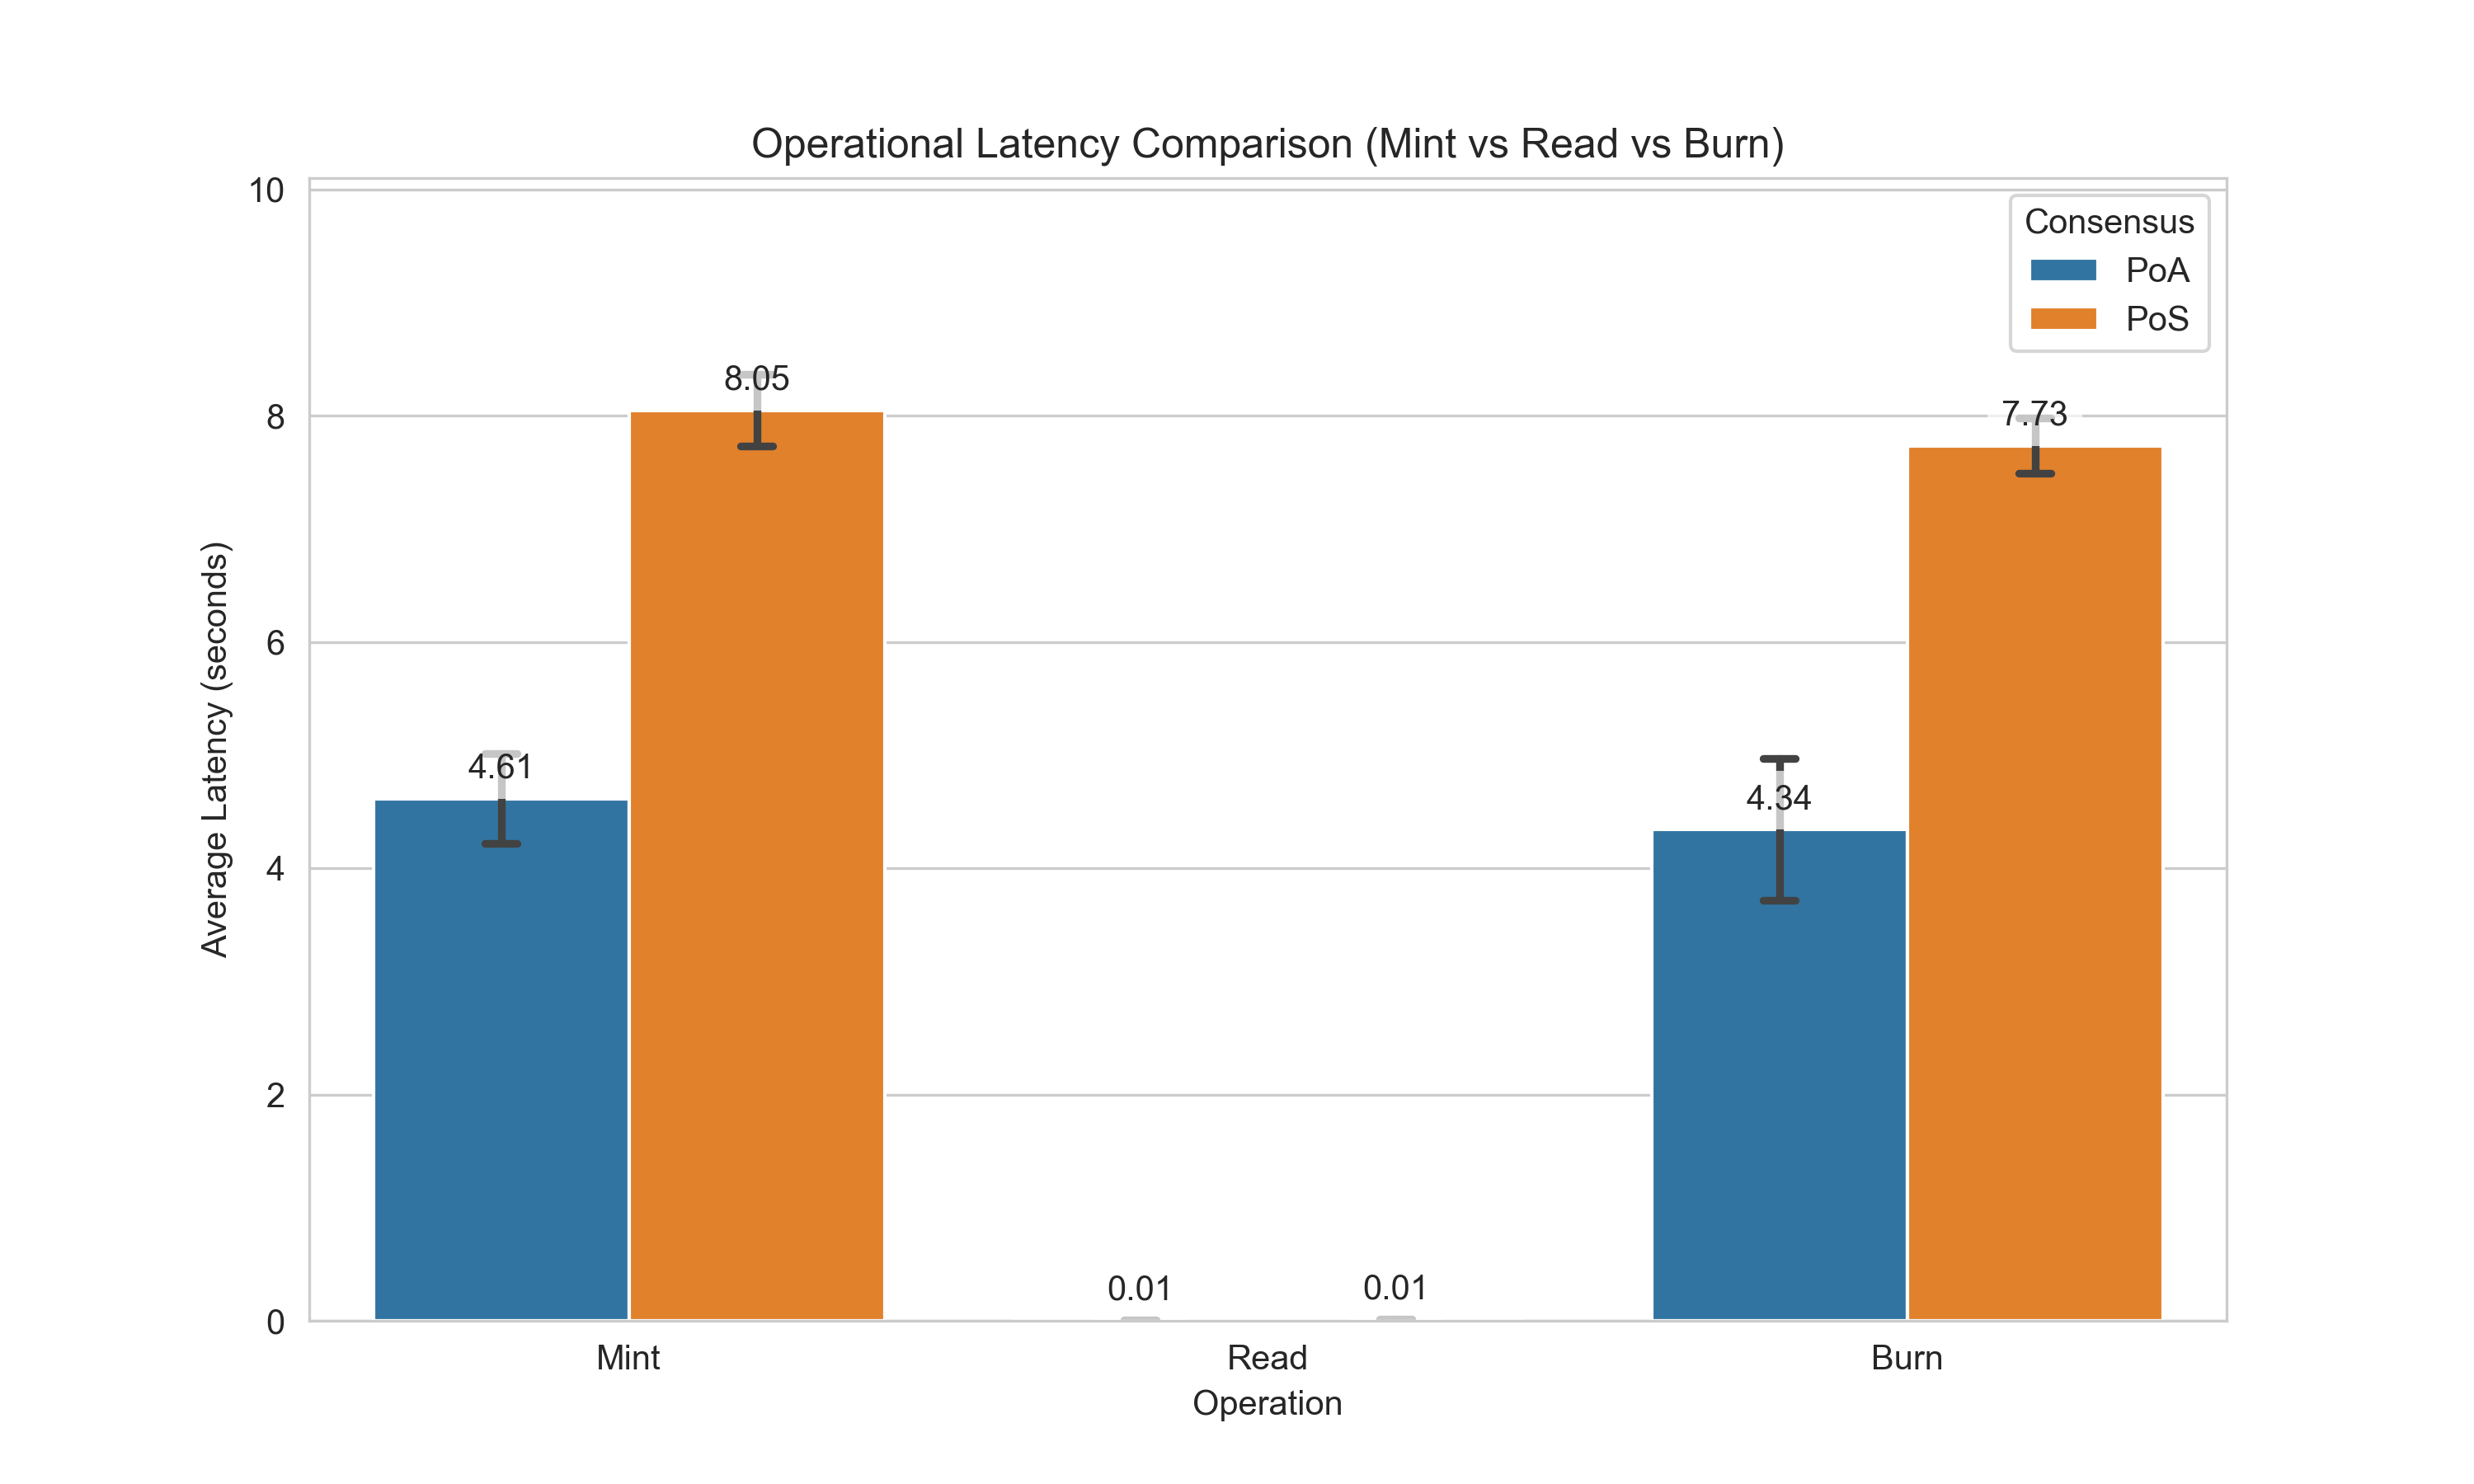
\includegraphics[width=0.9\textwidth]{images/lifecycle_latency_comparison.png}
    \caption{Perbandingan Latensi Operasi Lifecycle}
    \label{fig:lifecycle_latency}
\end{figure}

\begin{figure}[htbp]
    \centering
    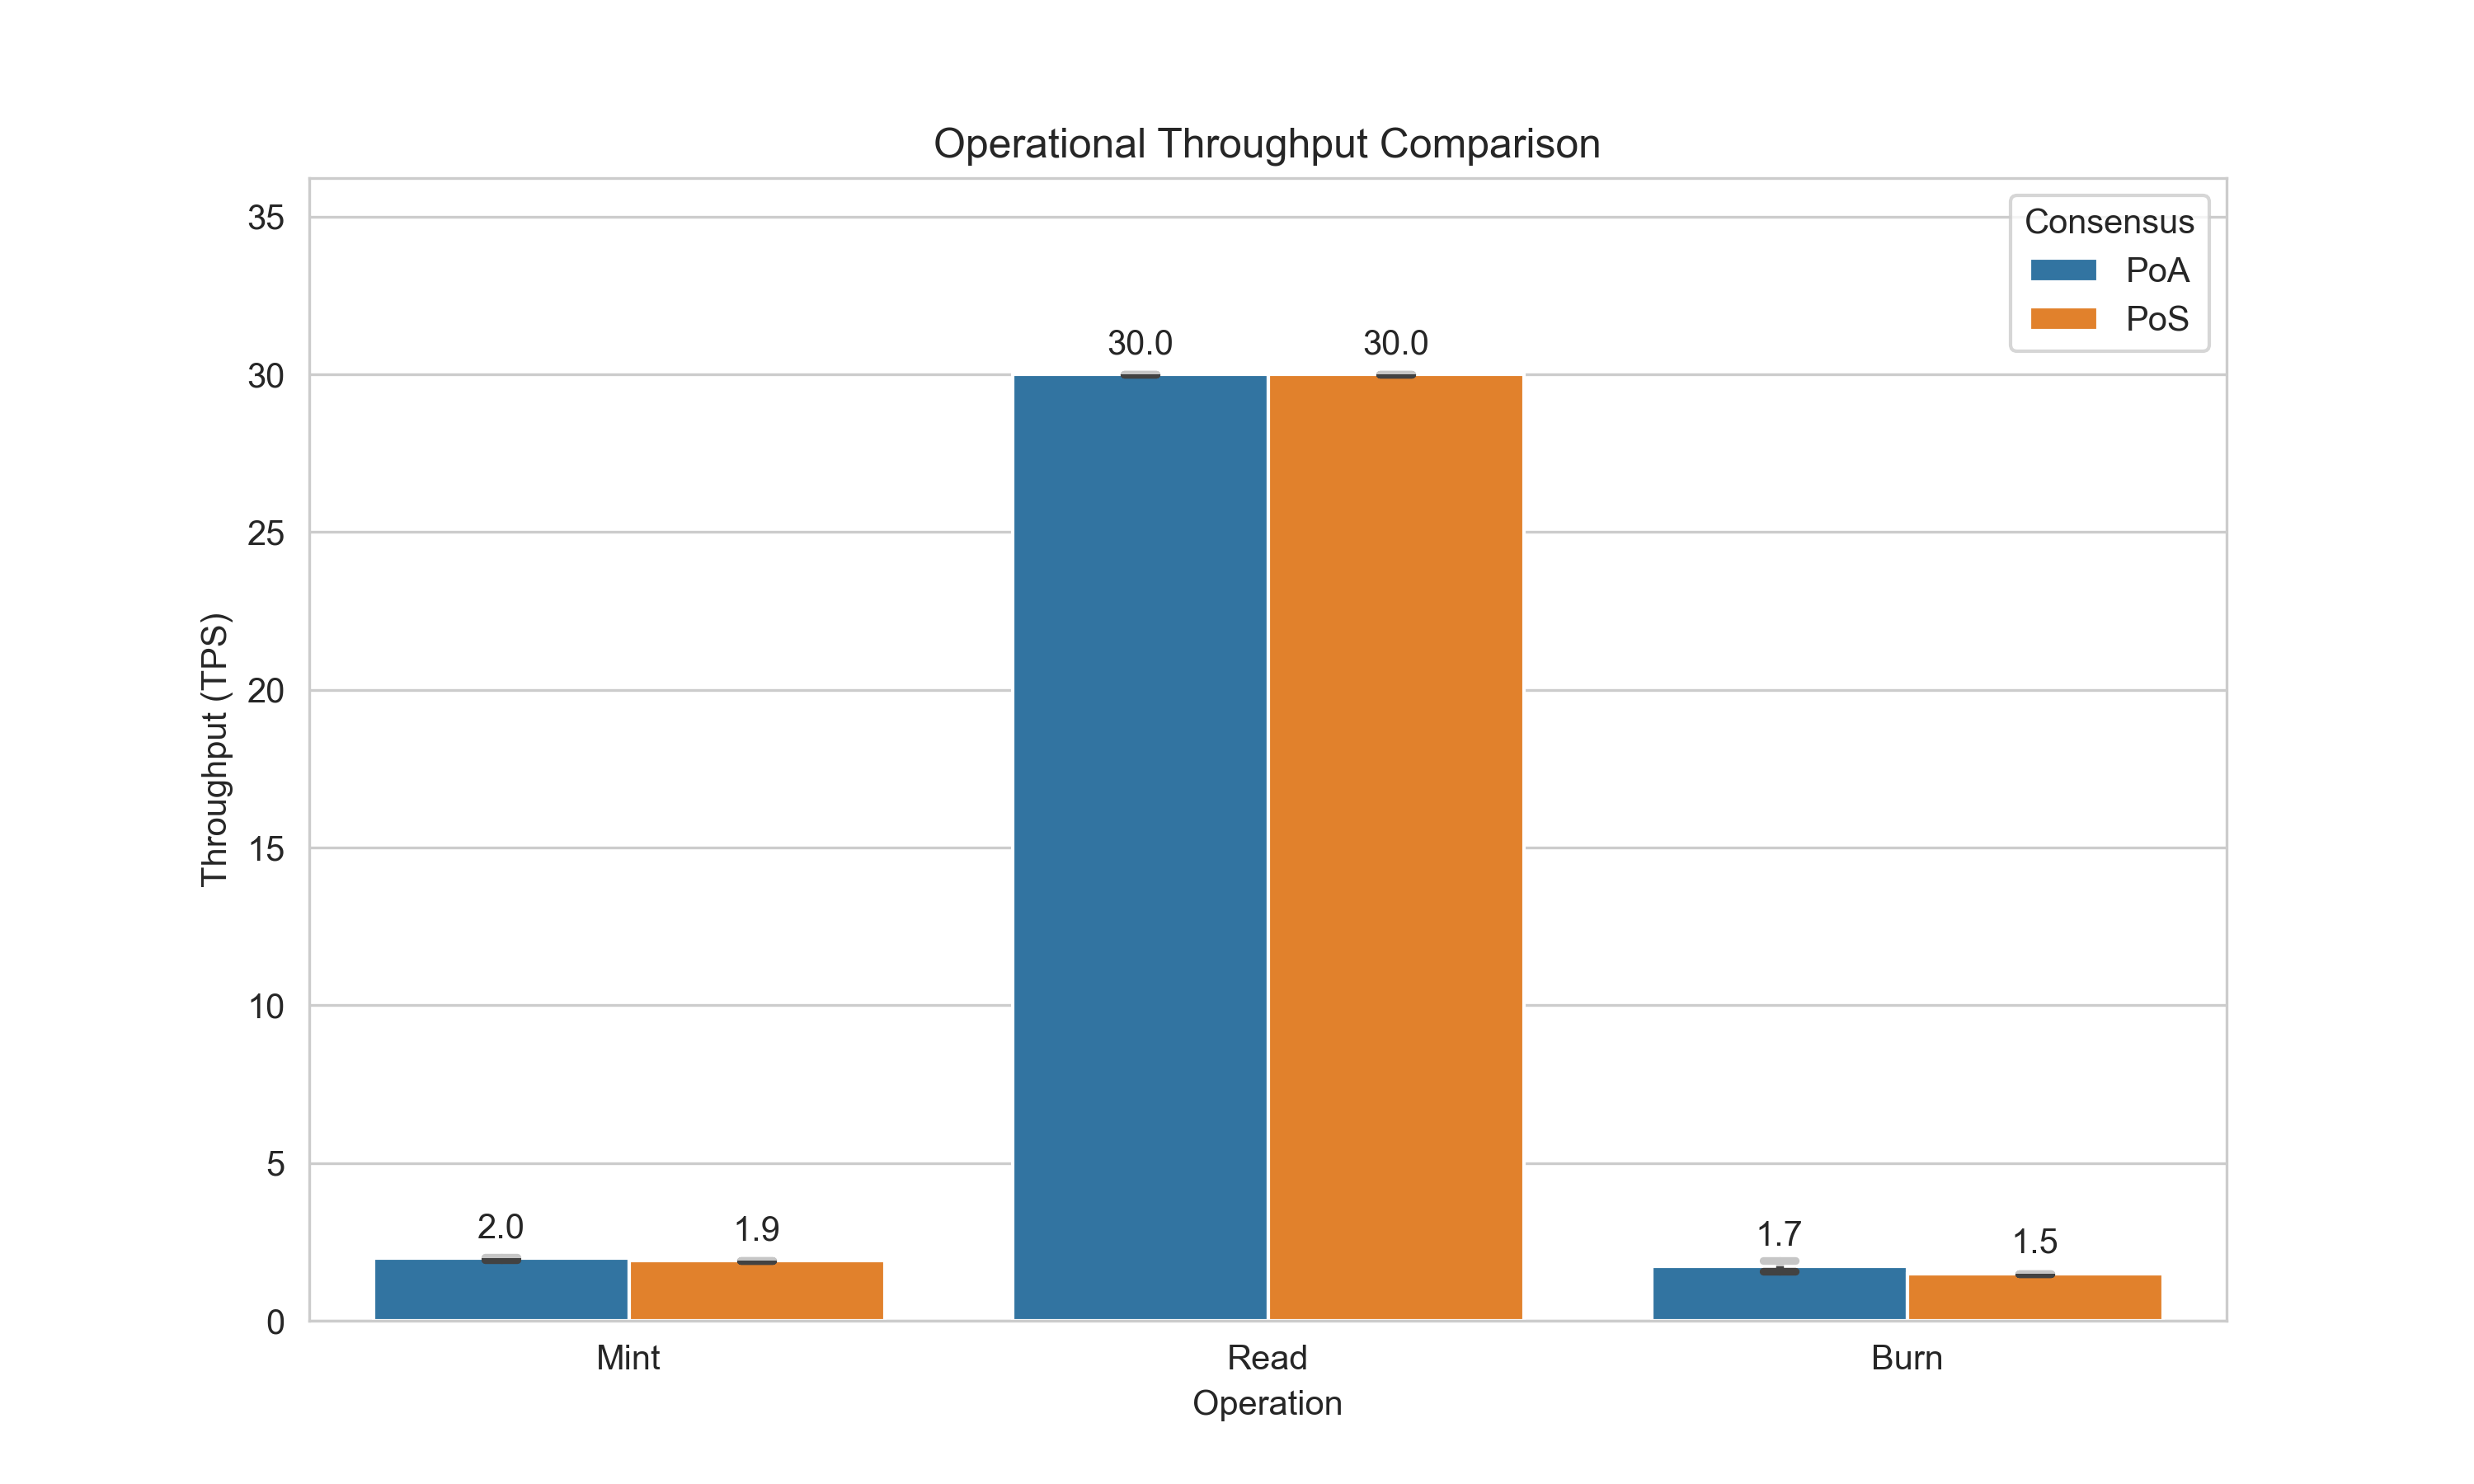
\includegraphics[width=0.9\textwidth]{images/lifecycle_tps_comparison.png}
    \caption{Perbandingan TPS Operasi Lifecycle}
    \label{fig:lifecycle_tps}
\end{figure}

\section{Analisis dan Pembahasan}

\subsection{Analisis Performa Throughput dan Skalabilitas}

Data menunjukkan fenomena menarik di mana PoS justru mencapai \textit{throughput} saturasi 2x lebih tinggi dibanding PoA pada skala kecil (4 Node). Hal ini diduga disebabkan oleh batasan \textit{Block Time}. PoA dengan blok 5 detik memiliki batas fisik jumlah gas/blok per satuan waktu. Sebaliknya, PoS dengan slot 12 detik, meskipun intervalnya lebih lama, memungkinkan \textit{batching} transaksi yang lebih efisien dengan batas gas yang sama per blok, menghasilkan \textit{throughput} agregat yang lebih tinggi sebelum saturasi RPC.

Namun, skalabilitas klien menunjukkan pola \textit{Sub-linear} untuk kedua konsensus, mengindikasikan bahwa \textit{bottleneck} utama bukan pada lapisan konsensus, melainkan pada lapisan RPC Node atau antrian transaksi di Caliper.

\subsection{Analisis Responsivitas dan Latensi}

PoA menunjukkan keunggulan telak dalam aspek responsivitas. Rata-rata latensi PoA (4.6 detik) sangat mendekati waktu blok (5 detik), menunjukkan inefisiensi minimal. Sebaliknya, PoS (8 detik) menderita latensi inheren dari mekanisme slot dan finalitas probabilistik awal. Untuk sistem layanan akademik, perbedaan 3--4 detik ini signifikan secara UX (\textit{User Experience}).

\subsection{Analisis Efisiensi dan Stabilitas}

PoA unggul dalam efisiensi sumber daya. PoS "membayar" desentralisasinya dengan komputasi mahal untuk \textit{attestation}. Stabilitas kedua sistem terbukti tangguh dalam uji jangka panjang (\textit{Soak Test}), tidak ditemukan indikasi kebocoran memori.

\subsection{Sintesis Visual: Trade-off Multidimensi}

Gambar \ref{fig:radar_chart} menyajikan sintesis karakteristik performa kedua konsensus dalam diagram radar lima dimensi. Setiap sumbu merepresentasikan skor 1-10 (semakin luar semakin baik).

Skor pada diagram ini merupakan hasil normalisasi kualitatif dari data kuantitatif yang diperoleh pada pengujian sebelumnya. Skala 1-10 digunakan untuk memvisualisasikan performa relatif, di mana nilai 10 merepresentasikan capaian terbaik dalam eksperimen ini. Sebagai contoh, pada dimensi \textit{Throughput}, PoS diberi skor 10 karena mencapai saturasi tertinggi ($\approx$60 TPS), sedangkan PoA diberi skor 5 karena hanya mencapai setengahnya ($\approx$30 TPS). Metode ini diterapkan secara konsisten pada dimensi lain untuk memudahkan pembandingan trade-off secara visual.

Interpretasi dari grafik tersebut adalah:
\begin{itemize}
    \item \textbf{Throughput (Capacity)}: PoS unggul signifikan (Skor 10), mencapai volume transaksi tertinggi.
    \item \textbf{Responsiveness}: PoA unggul (Skor 9) dengan latensi yang lebih rendah dan waktu blok lebih singkat.
    \item \textbf{Resource Efficiency}: PoA sangat dominan (Skor 9), sangat hemat CPU.
    \item \textbf{Stability}: Keduanya seimbang, namun PoA sedikit lebih stabil (CV Score lebih baik).
    \item \textbf{Finality Speed}: PoA Clique memberikan finalitas yang lebih cepat untuk aplikasi pengguna karena sifat deterministiknya.
\end{itemize}

Secara keseluruhan, PoA membentuk area grafik yang condong ke sisi efisiensi dan responsivitas, sedangkan PoS condong ke sisi kapasitas murni.

\begin{figure}[htbp]
    \centering
    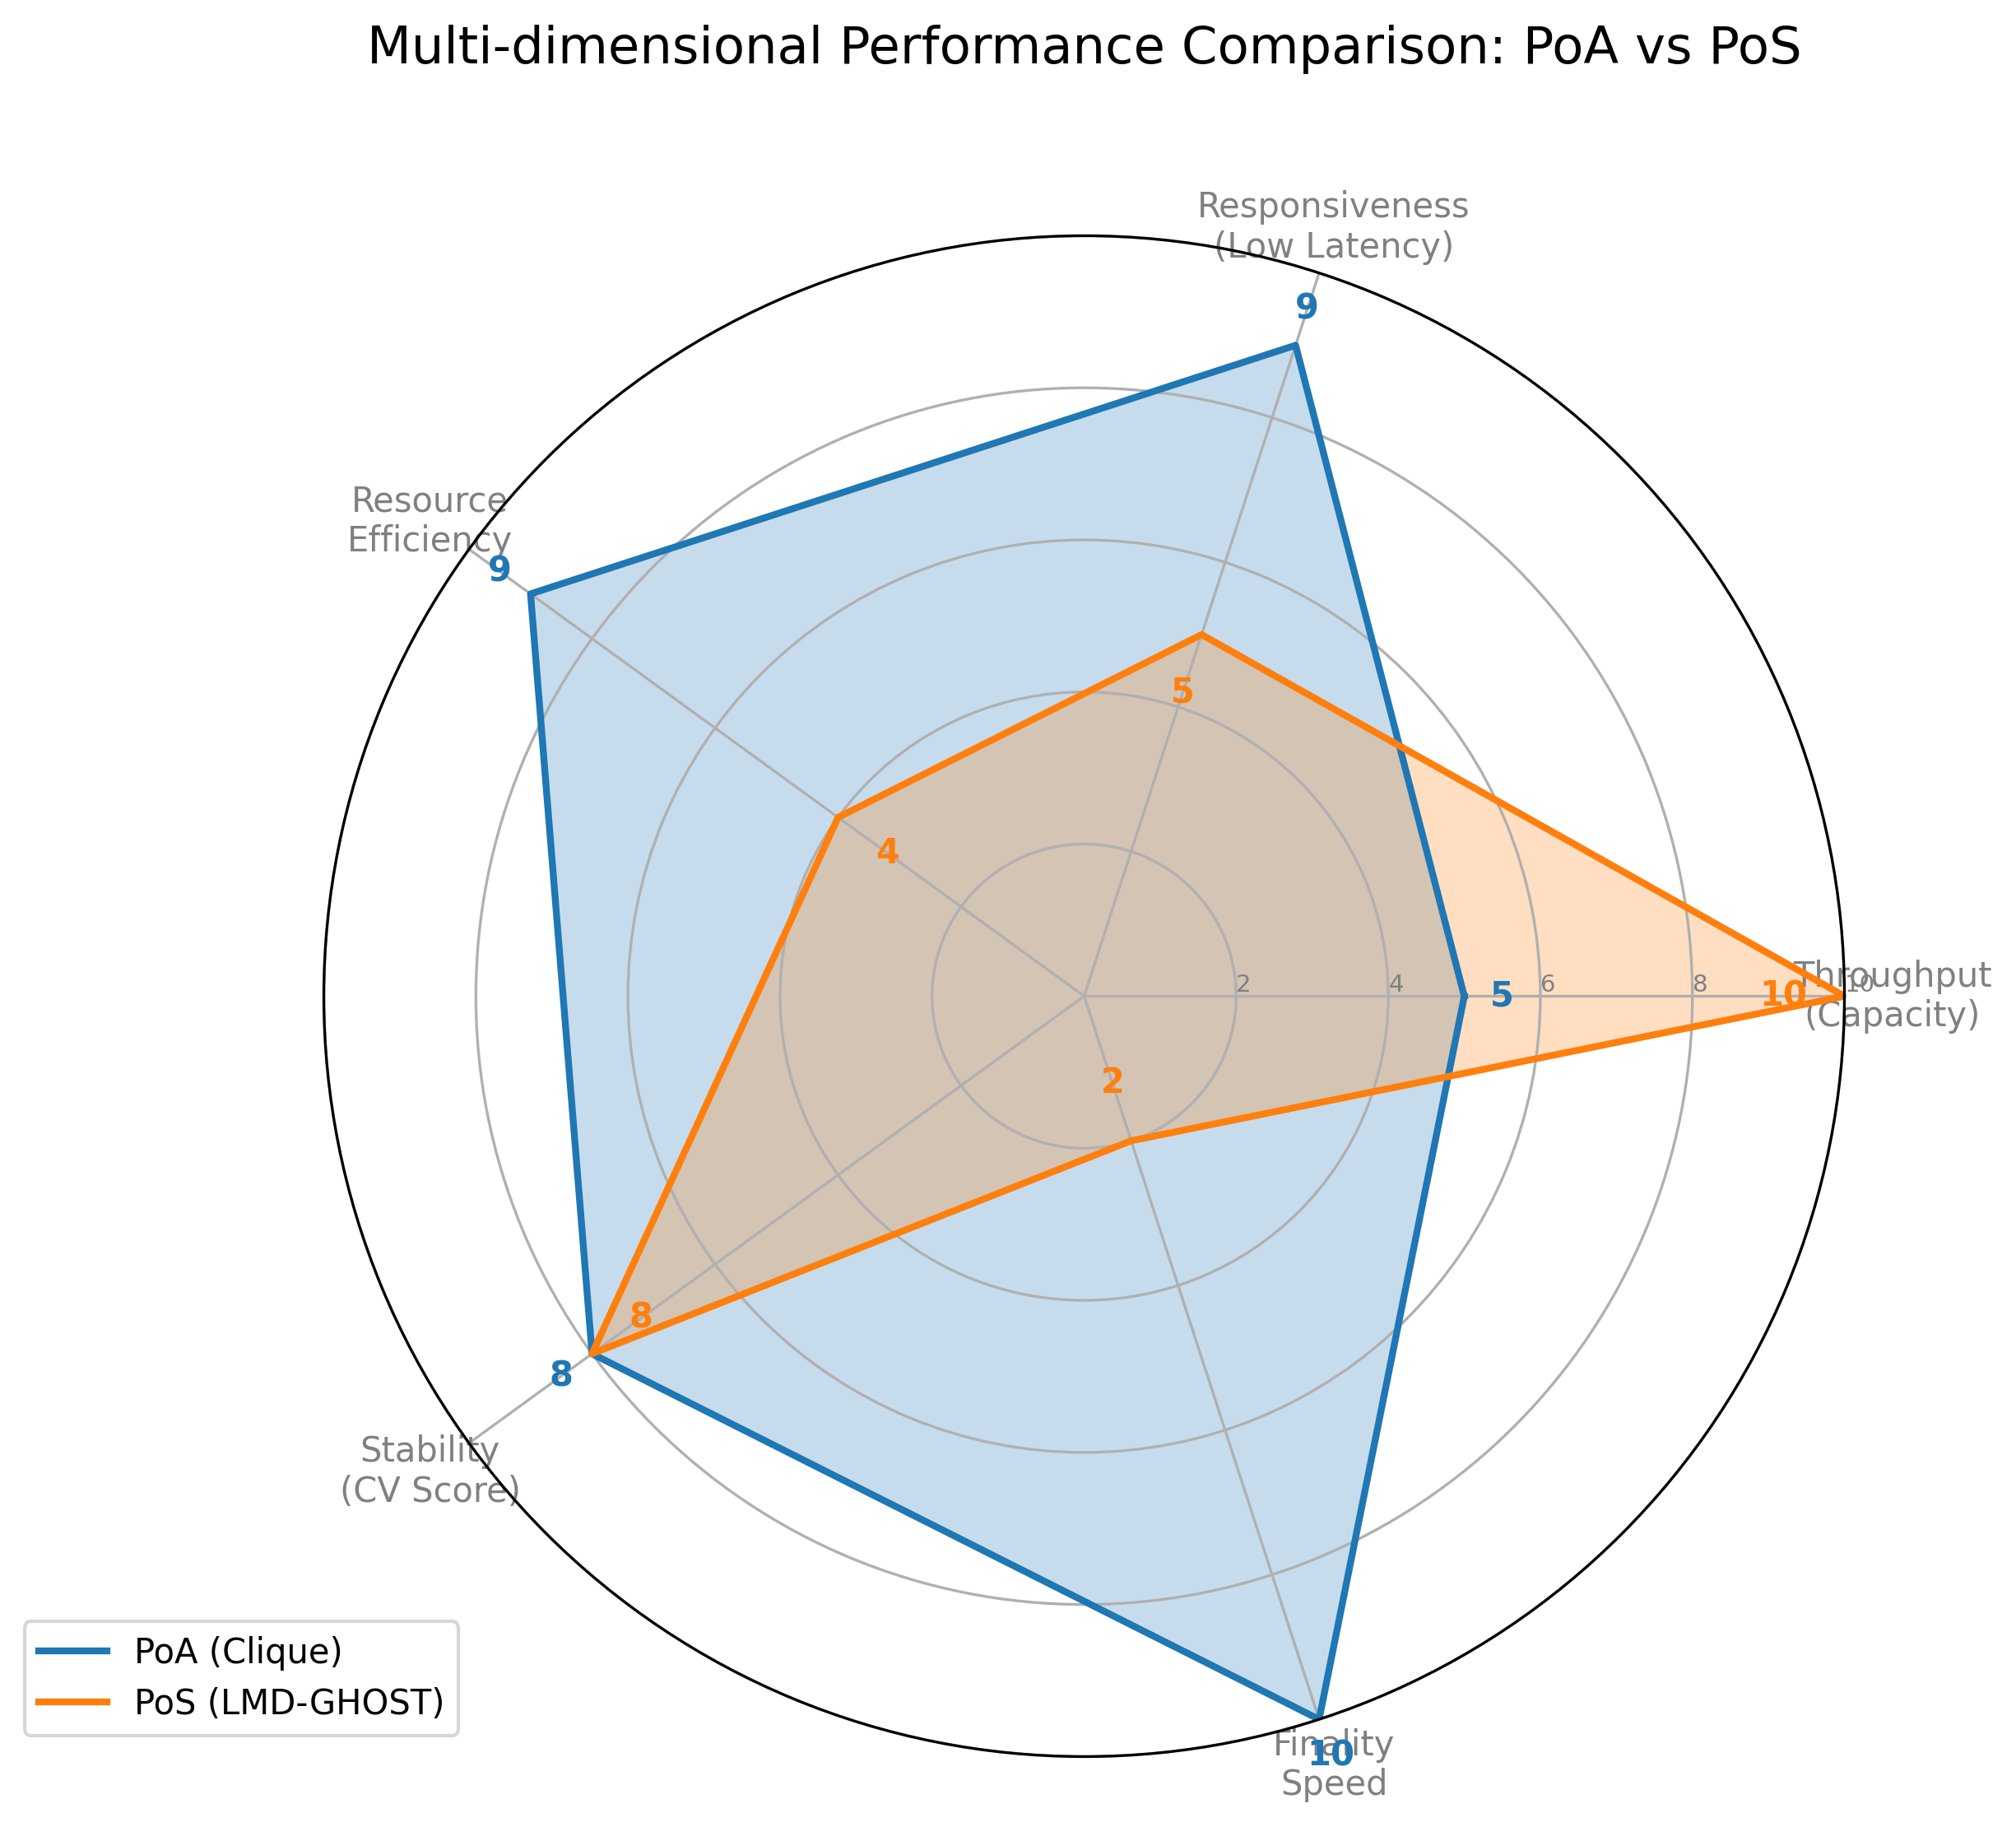
\includegraphics[width=0.8\textwidth]{images/radar_chart_comparison.png}
    \caption{Radar Chart Perbandingan PoA vs PoS}
    \label{fig:radar_chart}
\end{figure}

\subsection{Sintesis Akhir: Relevansi untuk DChain}
Untuk kasus penggunaan sertifikat akademik di DChain, karakteristik \textbf{PoA} terbukti lebih menguntungkan karena:
\begin{enumerate}
    \item \textbf{User-Interactive}: Latensi rendah memberikan pengalaman pengguna yang lebih baik.
    \item \textbf{Read-Heavy}: Volume transaksi tulis (penerbitan ijazah) relatif rendah dan musiman, sehingga kapasitas masif PoS kurang termanfaatkan dibanding efisiensi biaya operasional PoA.
    \item \textbf{Finalitas}: PoA Clique menawarkan finalitas deterministik yang lebih sederhana untuk integrasi aplikasi.
\end{enumerate}

\section{Perbandingan dengan Penelitian Terdahulu}

Penelitian ini memberikan kontribusi empiris dengan membandingkan hasil pengujian DChain terhadap literatur yang ada, sebagaimana dirangkum dalam Tabel \ref{tab:comparison_literature}.

\begin{table}[htbp]
\centering
\caption{Perbandingan Hasil DChain dengan Literatur Terdahulu}
\label{tab:comparison_literature}
\begin{tabularx}{\textwidth}{|>{\RaggedRight\arraybackslash}p{2.5cm}|>{\RaggedRight\arraybackslash}X|>{\RaggedRight\arraybackslash}X|>{\RaggedRight\arraybackslash}p{4cm}|}
\hline
\textbf{Aspek} & \textbf{Temuan DChain} & \textbf{Penelitian Terdahulu} & \textbf{Analisis} \\
\hline
\textbf{Throughput} & $\approx$30--40 TPS (Saturasi Awal) & PoA $>1000$ TPS \cite{choi2020,rebello2020} & Hasil DChain lebih rendah karena menggunakan VPS \textit{resource} terbatas dan latensi geografis nyata, mencerminkan kondisi riil. \\
\hline
\textbf{Latensi} & $\approx$4--5 detik & PoA $<1$ detik \cite{arslan2020,wicaksono2025} & Konsisten dengan konfigurasi \textit{block time} 5 detik. Penelitian Wicaksono \cite{wicaksono2025} juga menemukan latensi serupa pada \textit{load} moderat. \\
\hline
\textbf{Efisiensi} & Sangat Tinggi (TPS/\%CPU) & Dianggap efisien \cite{sharma2020,ali2020} & Validasi temuan bahwa PoA jauh lebih ringan dibanding PoS. \\
\hline
\end{tabularx}
\end{table}

Berdasarkan analisis pada Tabel \ref{tab:comparison_literature}, penelitian ini mengisi celah (\textit{research gap}) dengan:
\begin{enumerate}
    \item \textbf{Studi Kasus Spesifik}: Menguji beban kerja fungsional (\textit{Lifecycle}) yang relevan secara bisnis, bukan sekadar transfer token.
    \item \textbf{Topologi Geografis Nyata}: Simulasi latensi antar-kampus (UGM, UI, ITB), bukan \textit{localhost}.
    \item \textbf{Analisis Stabilitas}: Menambahkan uji \textit{Soak Test} untuk membuktikan ketahanan sistem.
\end{enumerate}